\documentclass{beamer}

% Thème
\usetheme[progressbar=frametitle]{metropolis} 
\usecolortheme{dove} 

% Paquets
\usepackage{graphicx}
\usepackage{booktabs}
\usepackage[french]{babel}
\usepackage[absolute,overlay]{textpos}
\usepackage{fontspec}
\usepackage{caption}
\usepackage{subcaption}
\usepackage[export]{adjustbox}

% Polices
\setsansfont{Fira Sans}
\setmonofont{Fira Code}

% Informations sur la présentation
\title{1924B Mini Boîte Noire}
\subtitle{Enregistreur de données de vol}
\author{Ali Zoubir}

\institute{Supérvisé par : Juan José Moreno}
\date{}

\begin{document}
	
\begin{frame}[plain]
	\maketitle
	\begin{textblock*}{2cm}(9cm,5cm) % {block width} (coords)	
		\includegraphics[width=1\linewidth]{../figures/AMPA}
	\end{textblock*}
	\begin{textblock*}{2cm}(9cm,6.5cm) % {block width} (coords)	
		
\includegraphics[width=1\linewidth]{../figures/ETML-ES}
	\end{textblock*}
\end{frame}

\begin{frame}{Sommaire}
	\tableofcontents
\end{frame}

\section{Introduction}

\begin{frame}{Introduction}	
	\begin{textblock*}{4cm}(1cm,1cm) % {block width} (coords)	
	\begin{figure}[h]
		\centering
		\includegraphics[width=1\linewidth]{../figures/boite-noire}
		\caption{Boîte noire}
		\label{fig:boite-noire}
	\end{figure}
	\end{textblock*}
	
	\begin{textblock*}{7cm}(5.5cm,1.5cm) % {block width} (coords)
		Les enregistreurs de données de vol jouent un rôle crucial pour la compréhension des phénomènes aéronautiques.
		
		Ce projet a pour but la collecte et le stockage des données de \textcolor{blue}{localisation} et de \textcolor{blue}{déplacement} au moyen d'une \textcolor{blue}{IMU} et d'un \textcolor{blue}{GPS/GNSS}.		
	\end{textblock*}
\end{frame}

\begin{frame}{Principe}	
	\begin{textblock*}{4.5cm}(1cm,1cm) % {block width} (coords)
	\begin{figure}[h]
		\centering
		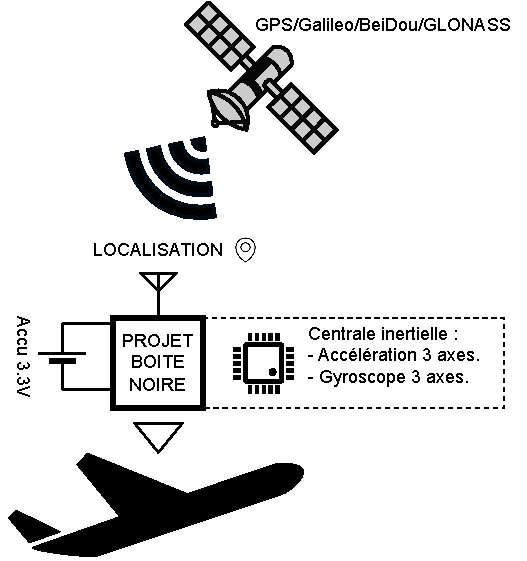
\includegraphics[width=1\linewidth]{../figures/cdc/schema_principe}
		\caption{Schéma de principe.}
		\label{fig:schemaprincipe}
	\end{figure}
	\end{textblock*}

	\begin{textblock*}{7cm}(5.5cm,1.5cm) 
	\begin{itemize}
		\item Données de localisation, trajectoire.
		\item Accéléromètre et Gyroscope.
		\item Miniaturisation.
		\item Bonne autonomie / Low power.
		\item Configuration des temps de sauvegardes.
		\item Charge, lecture et configuration par USB-C.
	\end{itemize}
	\end{textblock*}
\end{frame}

\section{Pré-étude}
\begin{frame}{Schéma bloc}
	\begin{figure}[h]
		\centering
		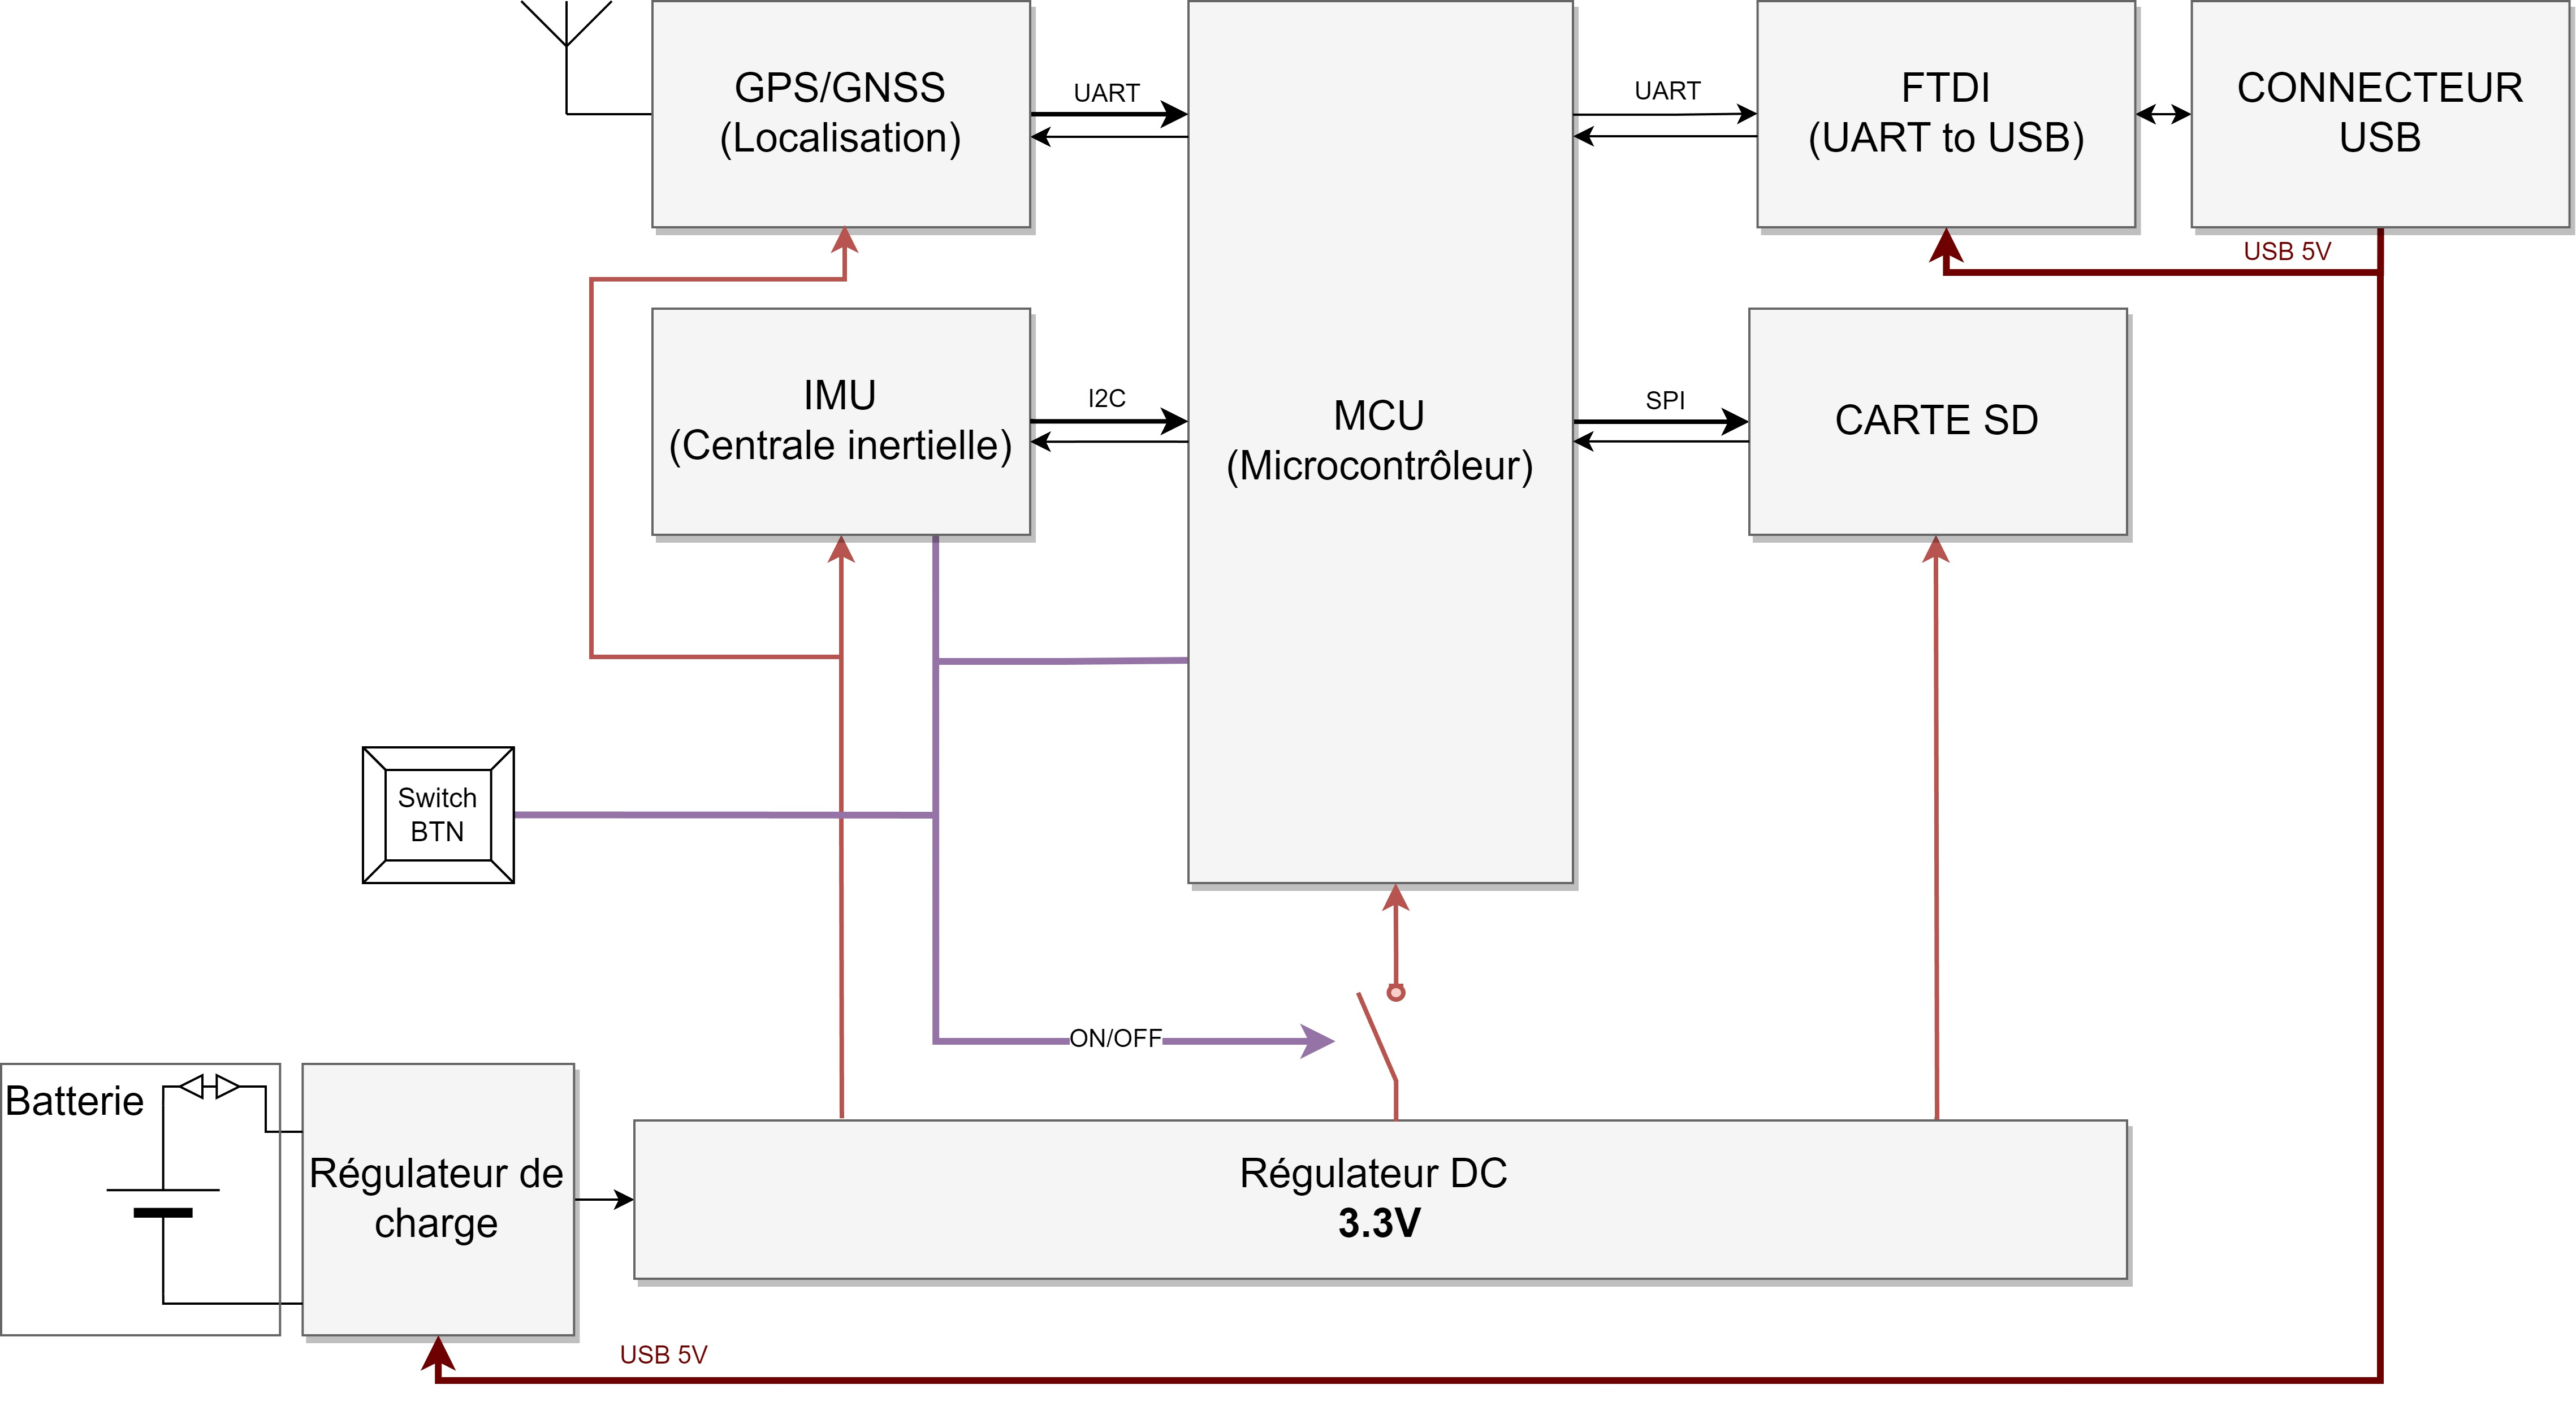
\includegraphics[width=1\textwidth]{../figures/cdc/blocs_grossiers_no_antenna}
		\caption{Schéma bloc.}
		\label{fig:schbloc}
	\end{figure}
\end{frame}

\begin{frame}{Choix des composants clés}
	\begin{tabular}{lll}
		Microcontrôleur &:& PIC32MX274F256D \\
		Centrale inertielle &:& BNO055 \\
		GNSS &:& CAM-M8C-0 \\
		Carte SD &:& 256MB \\
		Batterie &:& LI-ION 1600mAh \\
		Régulateur &:& MCP73871T-2CCI/ML\\
	\end{tabular}
\end{frame}

\begin{frame}{Microcontrôleur}
	\begin{figure}[h]
		\centering
		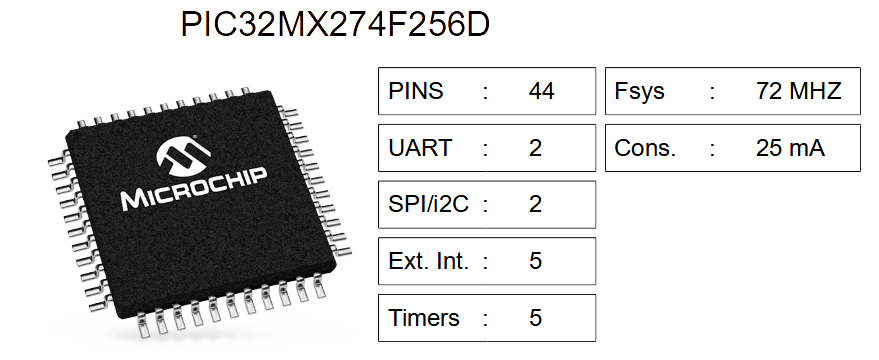
\includegraphics[width=0.7\linewidth]{../figures/pre_etude/Carac_PIC32}
		\caption{Caractéristiques PIC32.}
	\end{figure}
	Le MCU choisis dispose de différentes configurations de gestion de puissance, notamment des modes d'économie d'énergie, afin de permettre une meilleure autonomie. 
\end{frame}

\begin{frame}{Centrale inertielle}
	\begin{center}
		\begin{figure}[h]
			\centering
			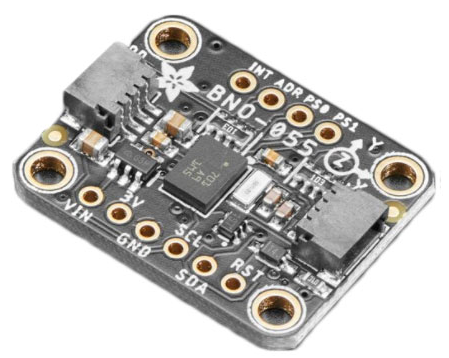
\includegraphics[width=0.25\linewidth]{../figures/pre_etude/BNO055_Adafruit}
			\caption{Illustration BNO055.}
		\end{figure} \vspace*{-2mm}
		
		\underline{Caractéristiques importantes :} \\
		\resizebox{.5\textwidth}{!}{\begin{tabular}{l l l l}
			Résolution gyroscope & : & 16 & [bits] \\
			Résolution accéléromètre & : & 14 & [bits] \\
			Résolution magnétomètre & : & $\sim$0.3 & [$\mu$T] \\
			$I_{DD}$ & : & 12.3 & [mA] \\
			Dérive de température & : & $\pm$ 0.03 & [\%/K] \\ 
			Dérive accéléromètre & : & 0.2 & [\%/V] \\
			Dérive gyroscope & : & <0.4 & [\%/V]
		\end{tabular}} \\
	\end{center}
\end{frame}

\begin{frame}{GNSS}
	\begin{figure}[h]
		\centering
		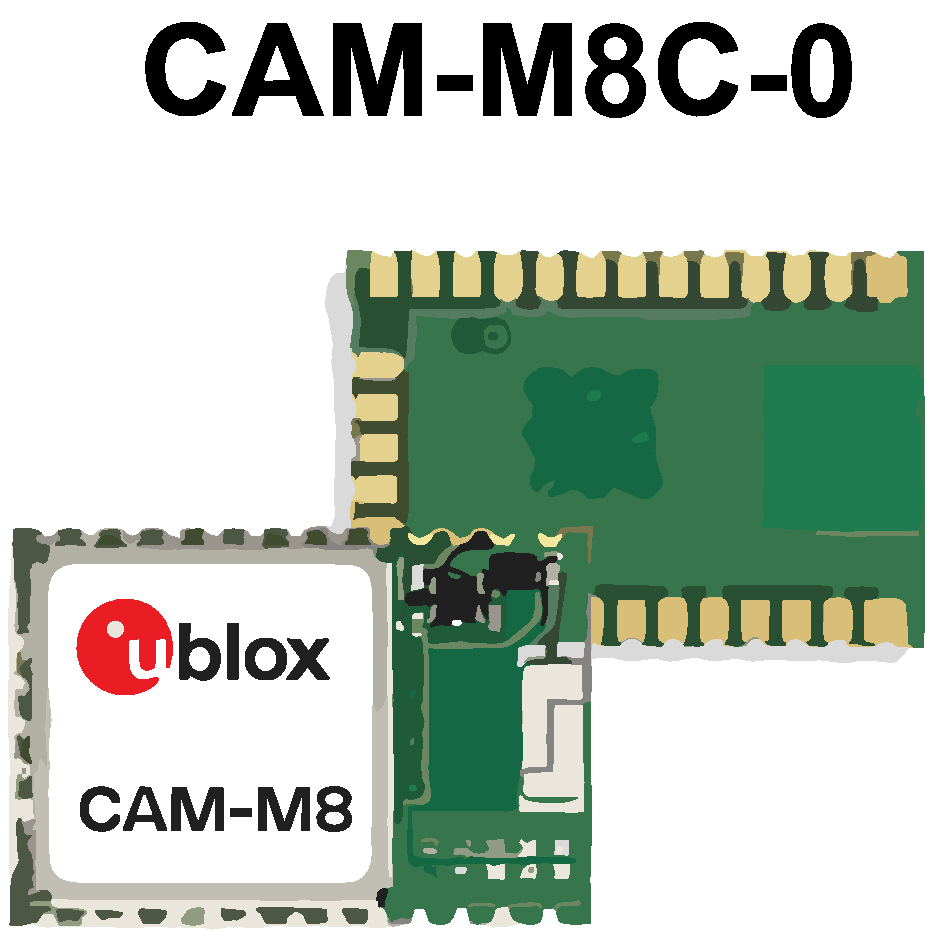
\includegraphics[width=0.25\linewidth]{../figures/pre_etude/img_gnss_crp}
	\end{figure}
	
	\begin{figure}[h]
		\centering
		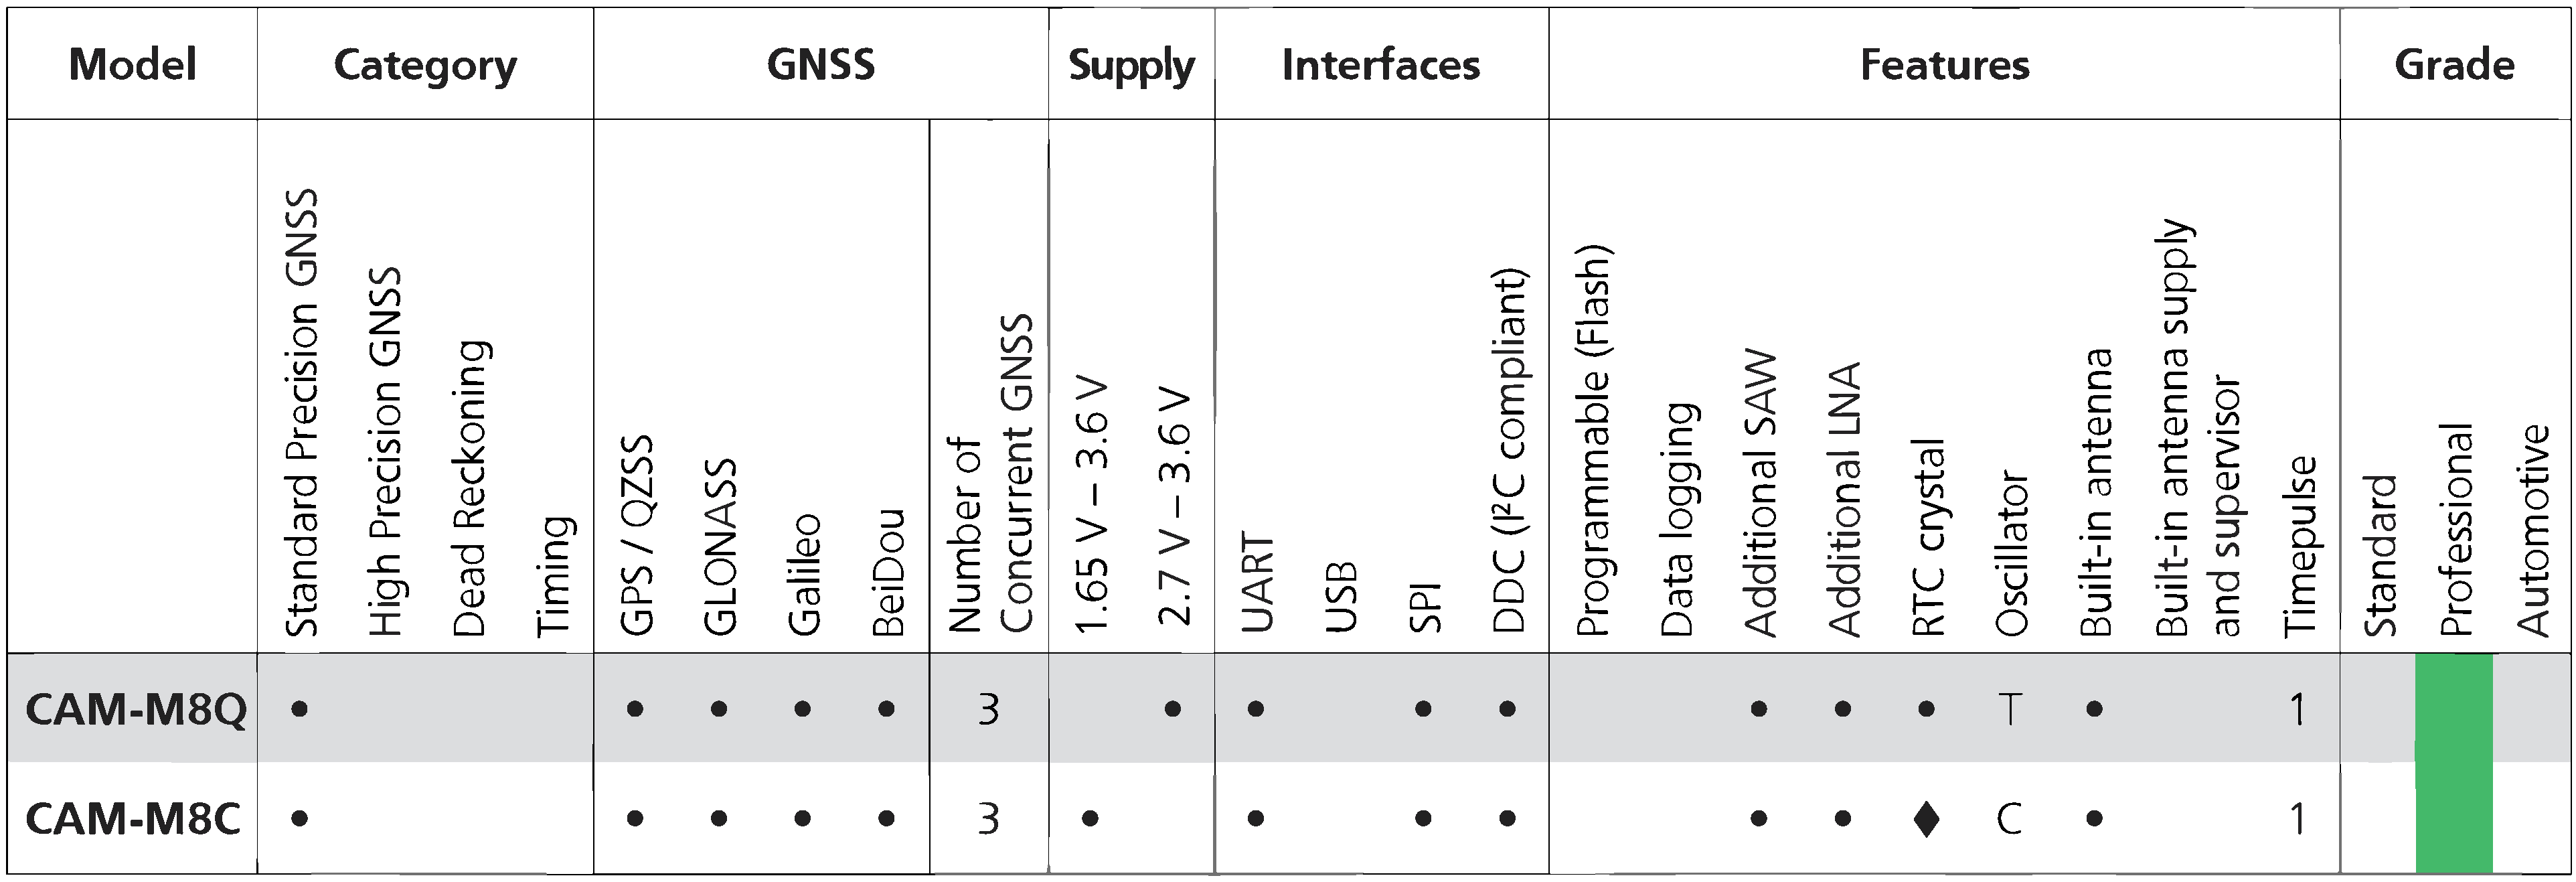
\includegraphics[width=.9\linewidth]{../figures/pre_etude/carac_GNSS}
		\caption{Caractéristiques du GNSS.}
		\label{fig:caracgnss}
	\end{figure}
\end{frame}

\begin{frame}{Carte SD}
	\begin{center}
	\resizebox{.4\textwidth}{!}{\begin{tabular}{lrl}
		$S_{SD}$ & $256$ & $[MB]$ \\
		$S_{gyro}$ & $16$ & $[Bytes]$ \\
		$S_{accel}$ & $16$ & $[Bytes]$ \\
		$S_{gnss}$ & $\sim100$ & $[Bytes]$ \\
		$T_{inertiel}$ & $0.5$ & $[s]$ \\
		$T_{gnss}$ & $5$ & $[s]$ \\
		$T_{mesMin}$ & $900$ & $[s]$ \\
	\end{tabular}}
	\end{center}\vspace*{-3mm}
	
	\begin{equation*}
		S_{single} = \frac{T_{gnss}}{T_{inertiel}}S_{accel} + S_{gnss} = \frac{5}{0.5}16 + 100 = 260 \; [Bytes]
	\end{equation*}\vspace*{-10mm}
	
	\begin{equation*}
		S_{mesures} = \frac{S_{single}}{T_{gnss}} * T_{mesMin} = \frac{260}{5} * 900 = 46'800 \; [Bytes] = 49.8 \; [KB]
	\end{equation*}\vspace*{-10mm}
	
	\begin{equation*}
		T_{mesures} = \frac{S_{SD}*T_{gnss}}{S_{single}} = \frac{256*10^6*5}{260} = \sim82'051 \; Minutes = \sim1368 \; H.
	\end{equation*}
\end{frame}

\begin{frame}{Batterie}
	\begin{center}
		\underline{Liste des consommations principales} \\
		\begin{table}[h]
			\centering
			\begin{tabular}{lrll}
				Microcontrôleur & 24 & [mA] & Typ. \\
				Carte-SD & ~100 & [mA] & Max. \\
				Carte-SD & ~60 & [mA] & Moyenne \\
				IMU & 12.3 & [mA] & Typ. \\
				GNSS & 71 & [mA] & Max. \\
				GNSS & 29 & [mA] & Typ. \\
				\hline
				Totale max & \underline{207.3} & [mA] & Max. \\
				Totale moyennes & \underline{125.3} & [mA] & Moyenne \\
				\hline
			\end{tabular}
			\caption{Tableau des consommations de courant.}
			\label{tab:consommateur}
		\end{table}
	\end{center}
	Temps minimum avec tolérance désiré : $10h \Rightarrow$ $\min\sim1300mAh$
\end{frame}

\begin{frame}{Synthèse pré-étude}
	\textbf{Choix des composants et technologies:}
	\begin{itemize}
		\item \textit{\textbf{Microcontrôleur}}: PIC32MX274F256D privilégié, 2 UART, 1 SPI, 1 I2C, économie d'énergie.
		\item \textit{\textbf{Centrale inertielle}}: BNO055 de BOSCH, mesures avancées, facile à implémenter.
		\item \textit{\textbf{GPS/GNSS}}: CAM-M8C-0 d'ublox, antenne interne omnidirectionnelle, facile à implémenter.
		\item \textit{\textbf{Carte SD}}: Capacité de 256MB, suffisante pour données de vol.
		\item \textit{\textbf{Batterie}}: Nécessité de 1253 mAh pour autonomie minimale.
	\end{itemize}
\end{frame}

\section{Développement schématique}

\begin{frame}{Blocs du systèmes}
	\begin{figure}[h]
		\centering
		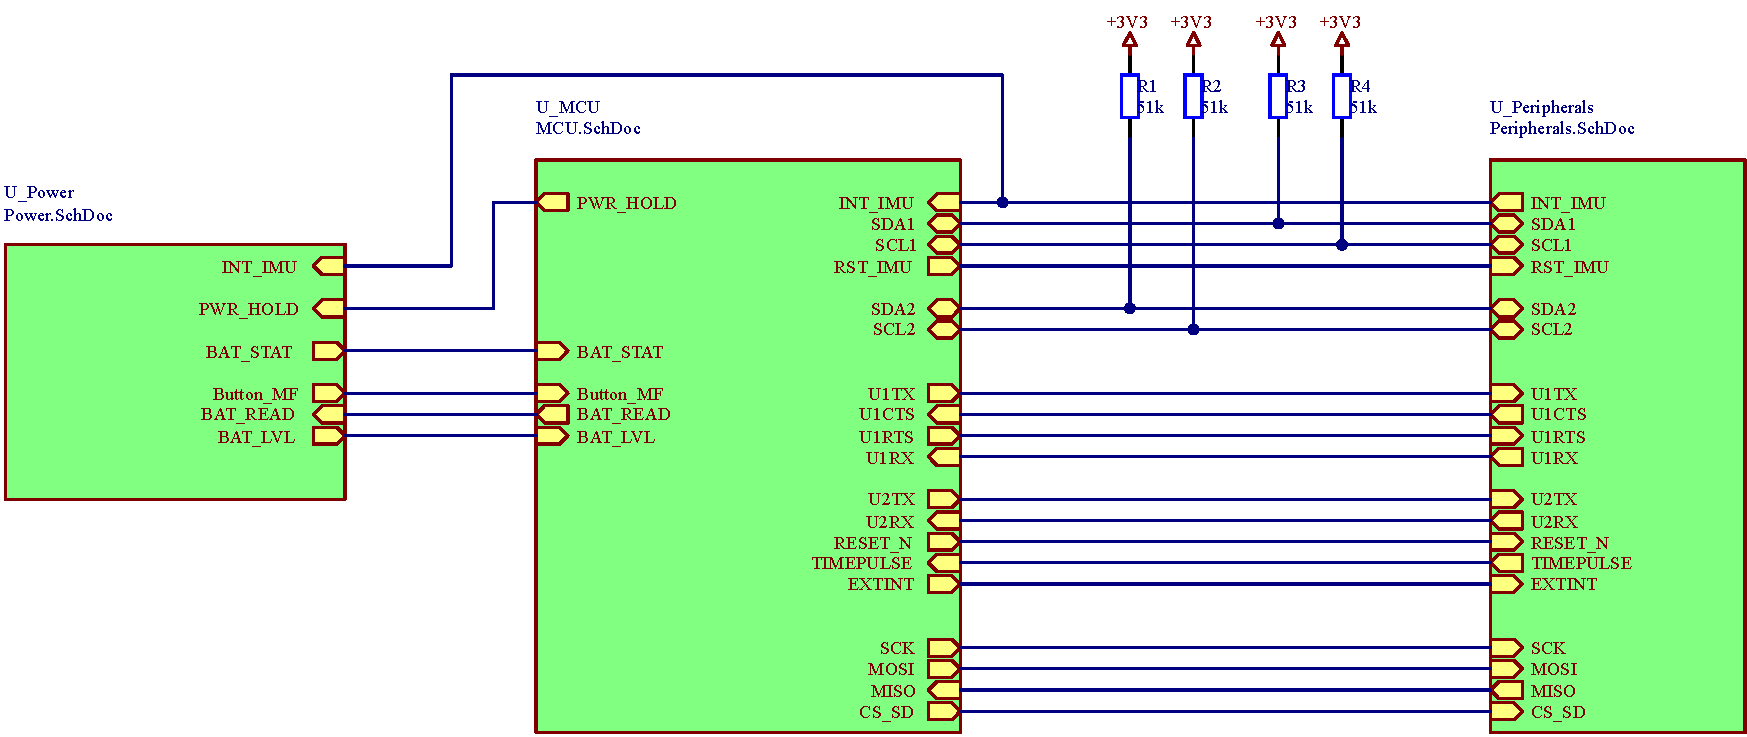
\includegraphics[width=1\linewidth]{../figures/etude/sch/BLOCS}
		\caption{Blocs du système.}
		\label{fig:blocs}
	\end{figure}
\end{frame}

\begin{frame}{MCU - Microcontrôleur}
	\begin{figure}[h]
		\centering
			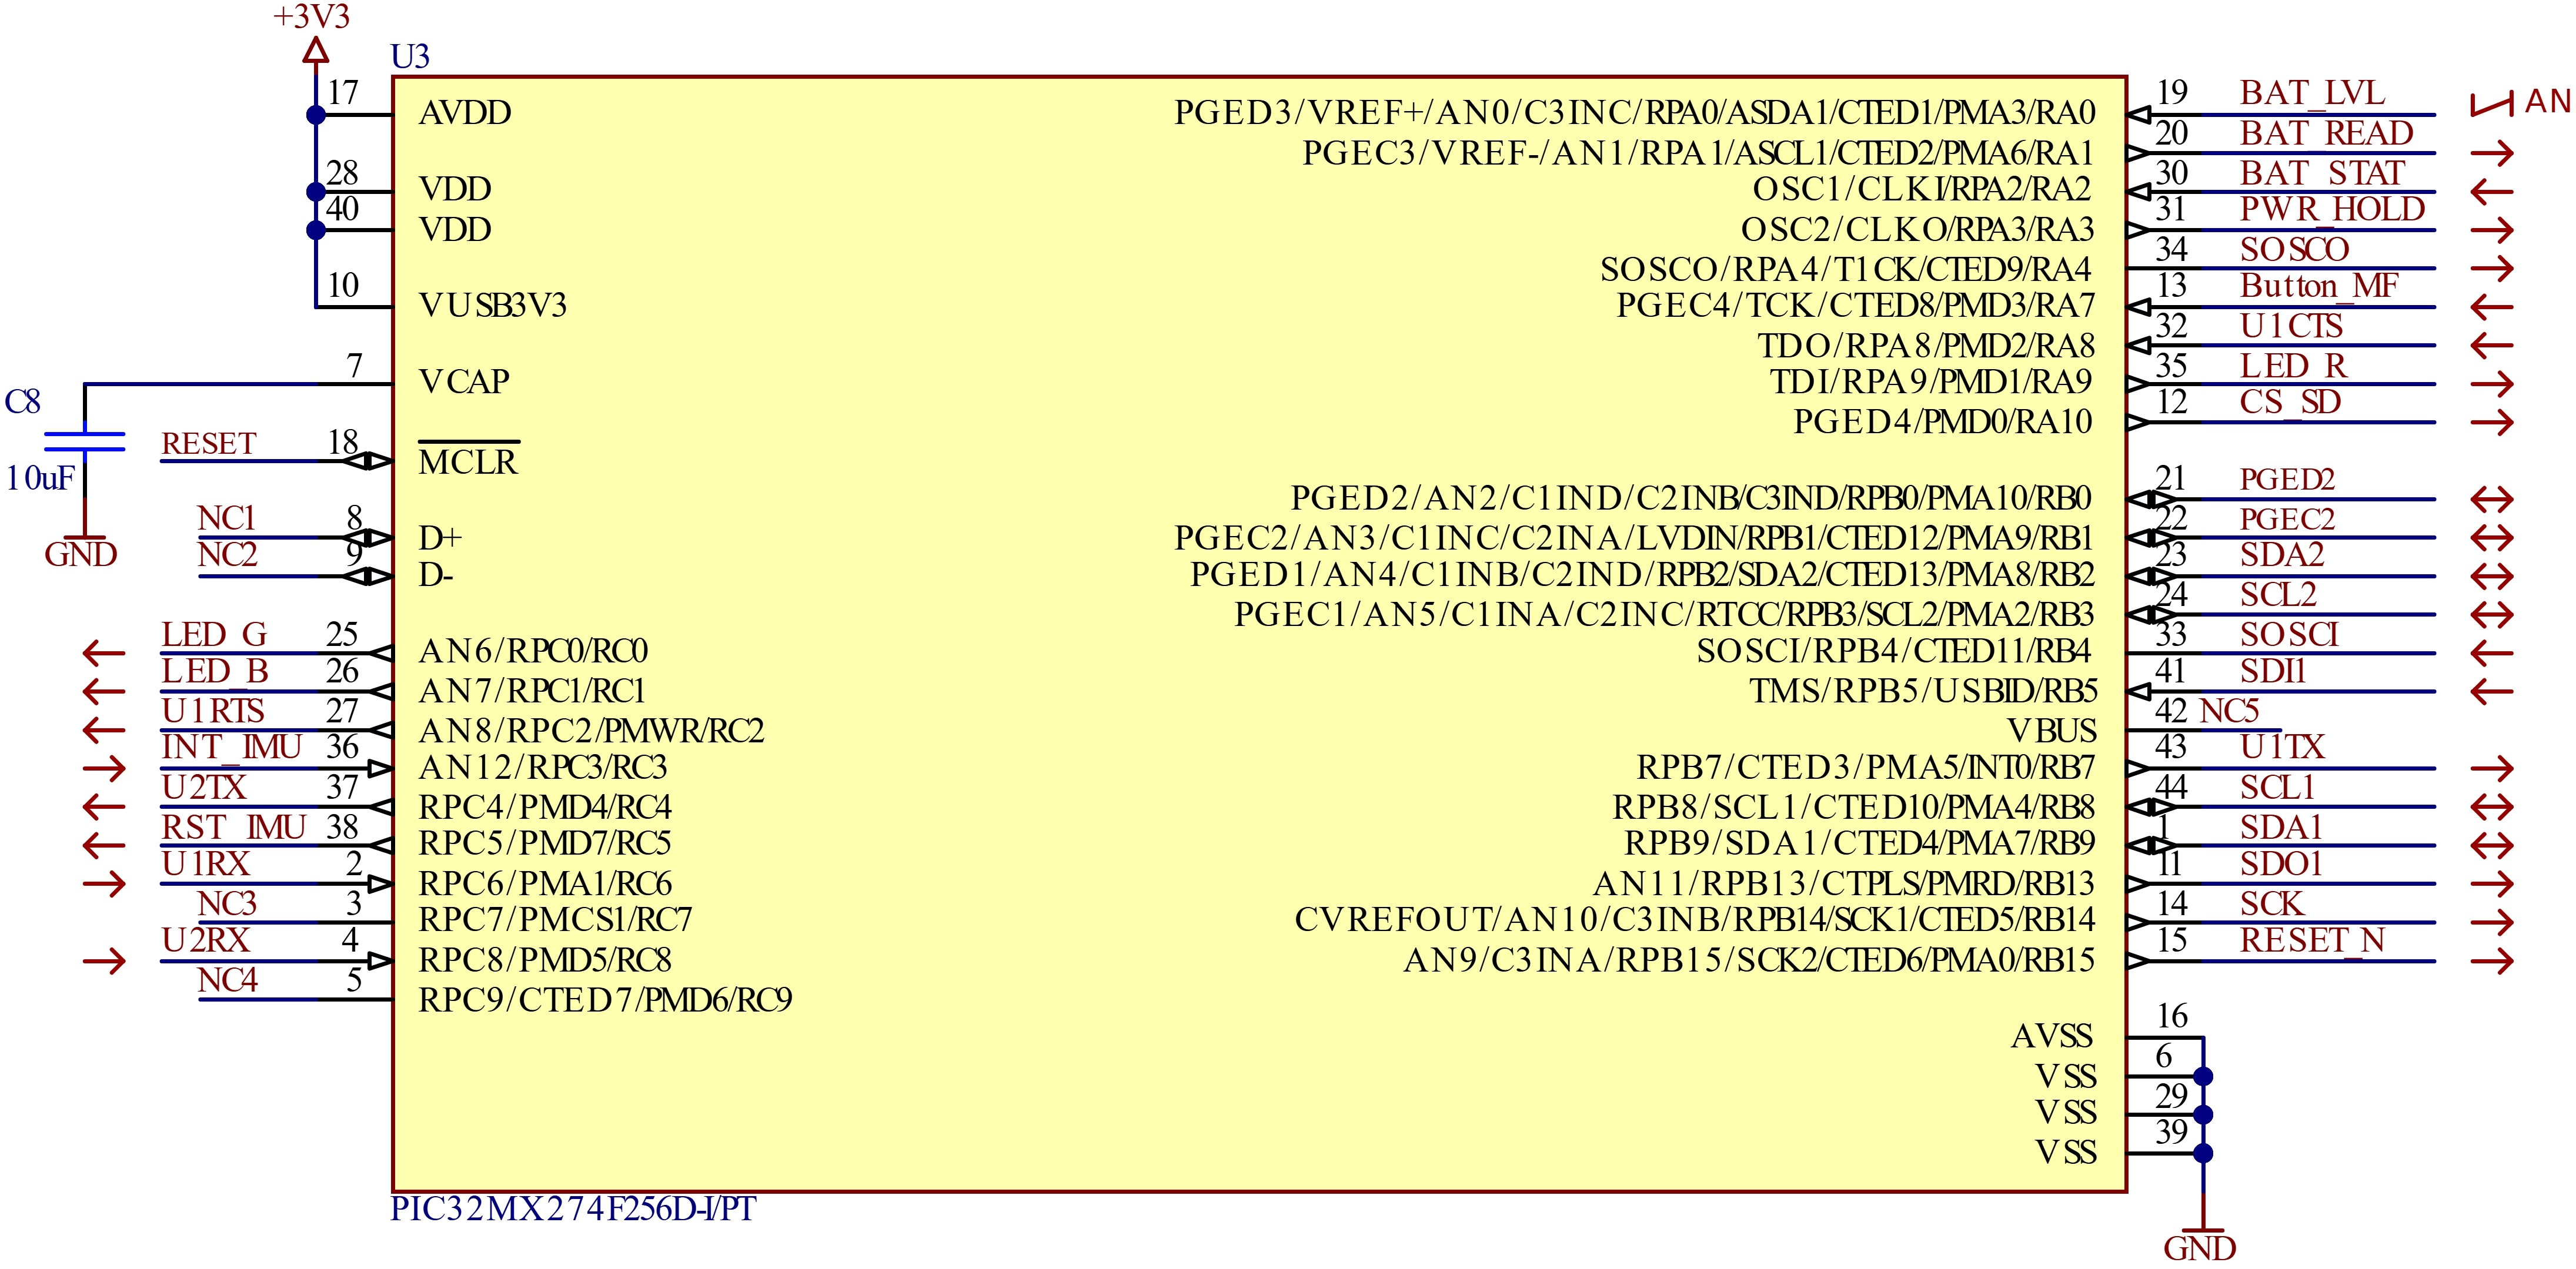
\includegraphics[width=1\linewidth]{../figures/etude/sch/MCU}
		\caption{Connexions du microcontrôleur}
		\label{fig:mcu}
	\end{figure}
\end{frame}

\begin{frame}{Peripherals - Carte SD}
	\begin{figure}[h]
		\centering
		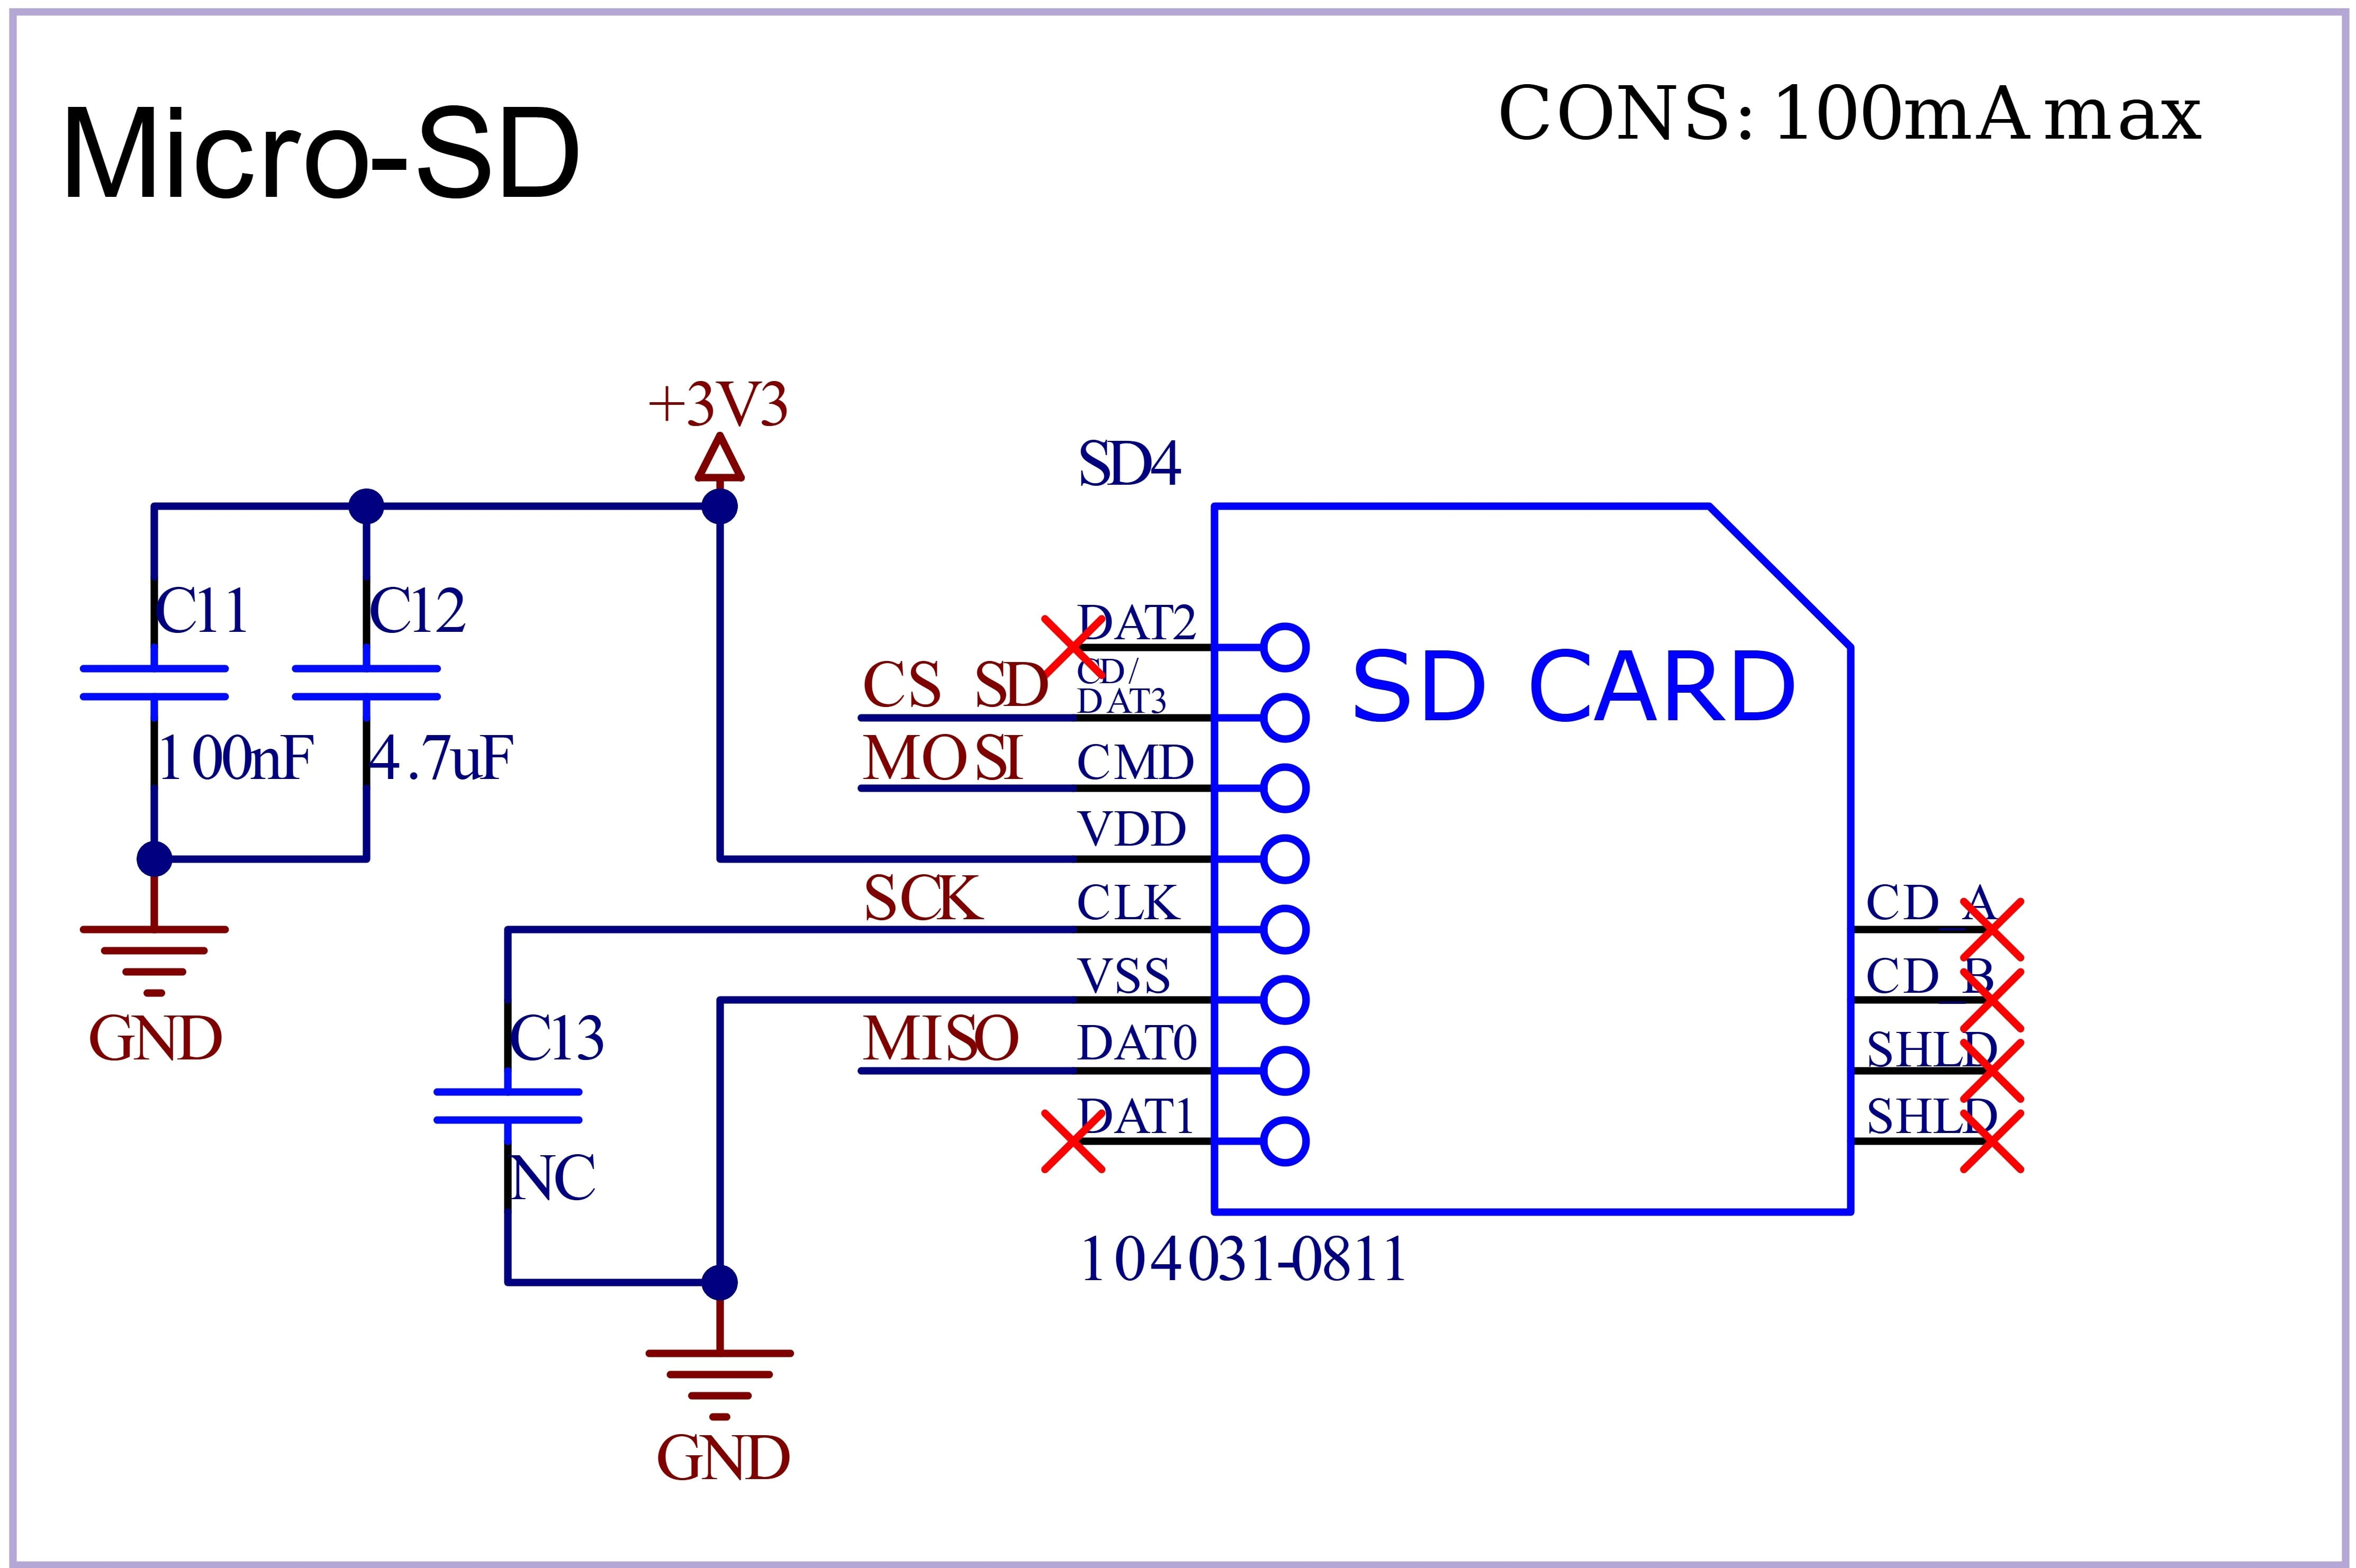
\includegraphics[width=.9\linewidth]{../figures/etude/sch/Carte-SD}
		\caption{Branchement carte SD.}
		\label{fig:carte-sd}
	\end{figure}
\end{frame}

\begin{frame}{Peripherals - Centrale inertielle}
	\begin{figure}[h]
		\centering
		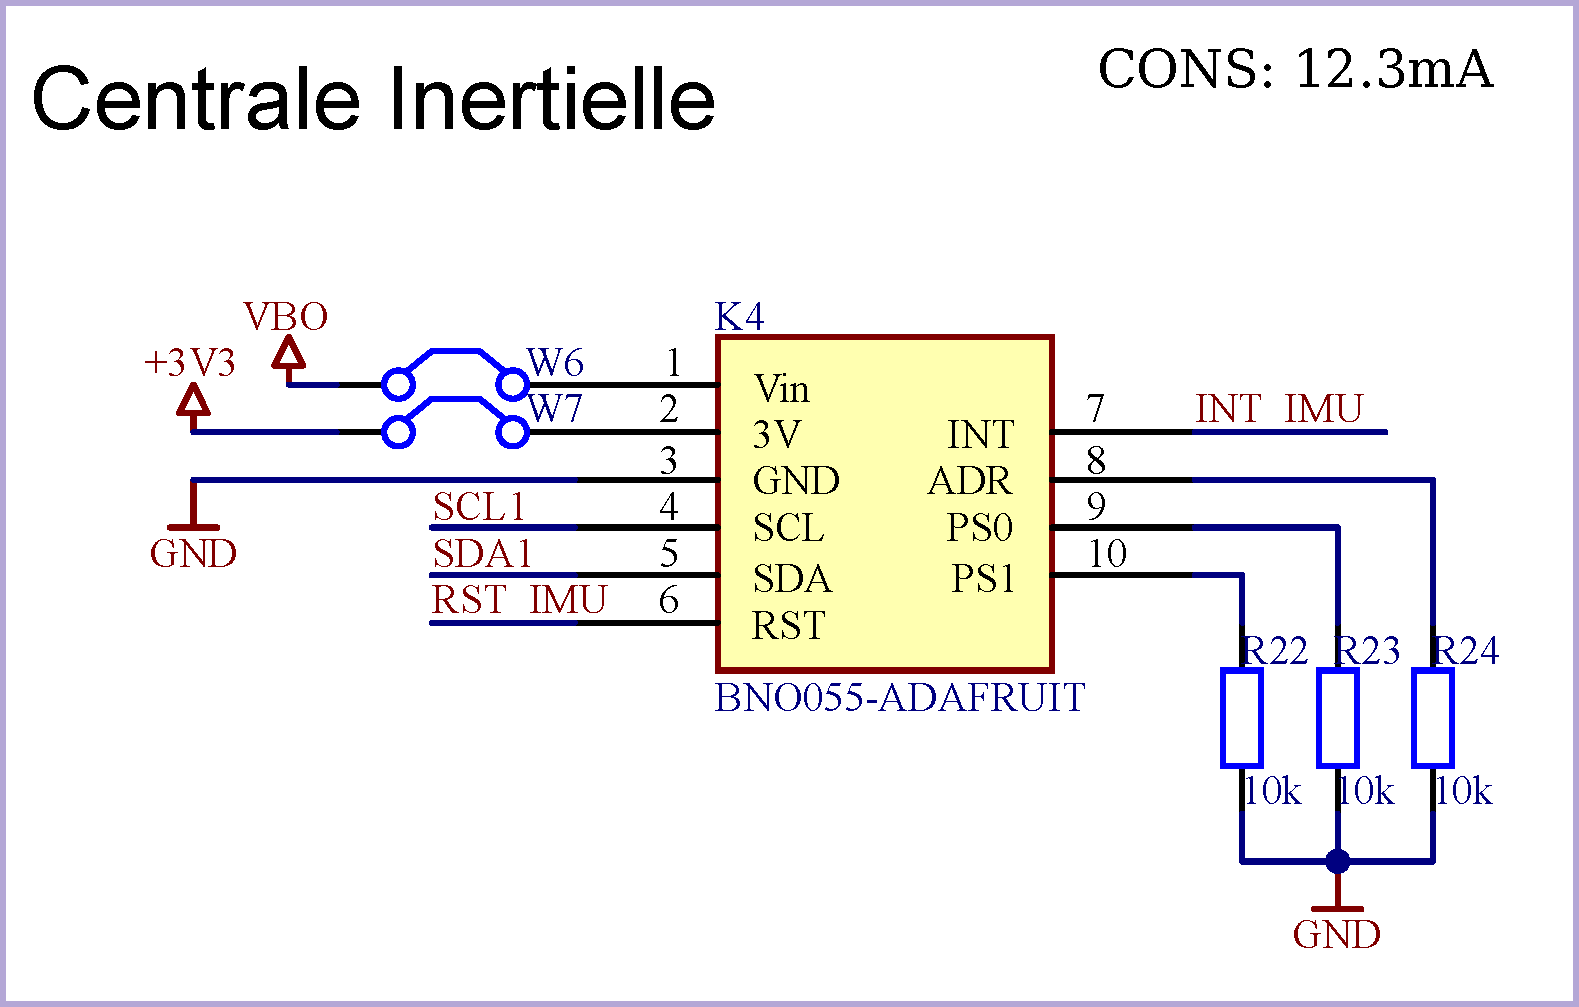
\includegraphics[width=.9\linewidth]{../figures/etude/sch/IMU}
		\caption{Schéma centrale inertielle.}
		\label{fig:imu}
	\end{figure}
\end{frame}

\begin{frame}{Peripherals - GNSS}
	\begin{figure}[h]
		\centering
		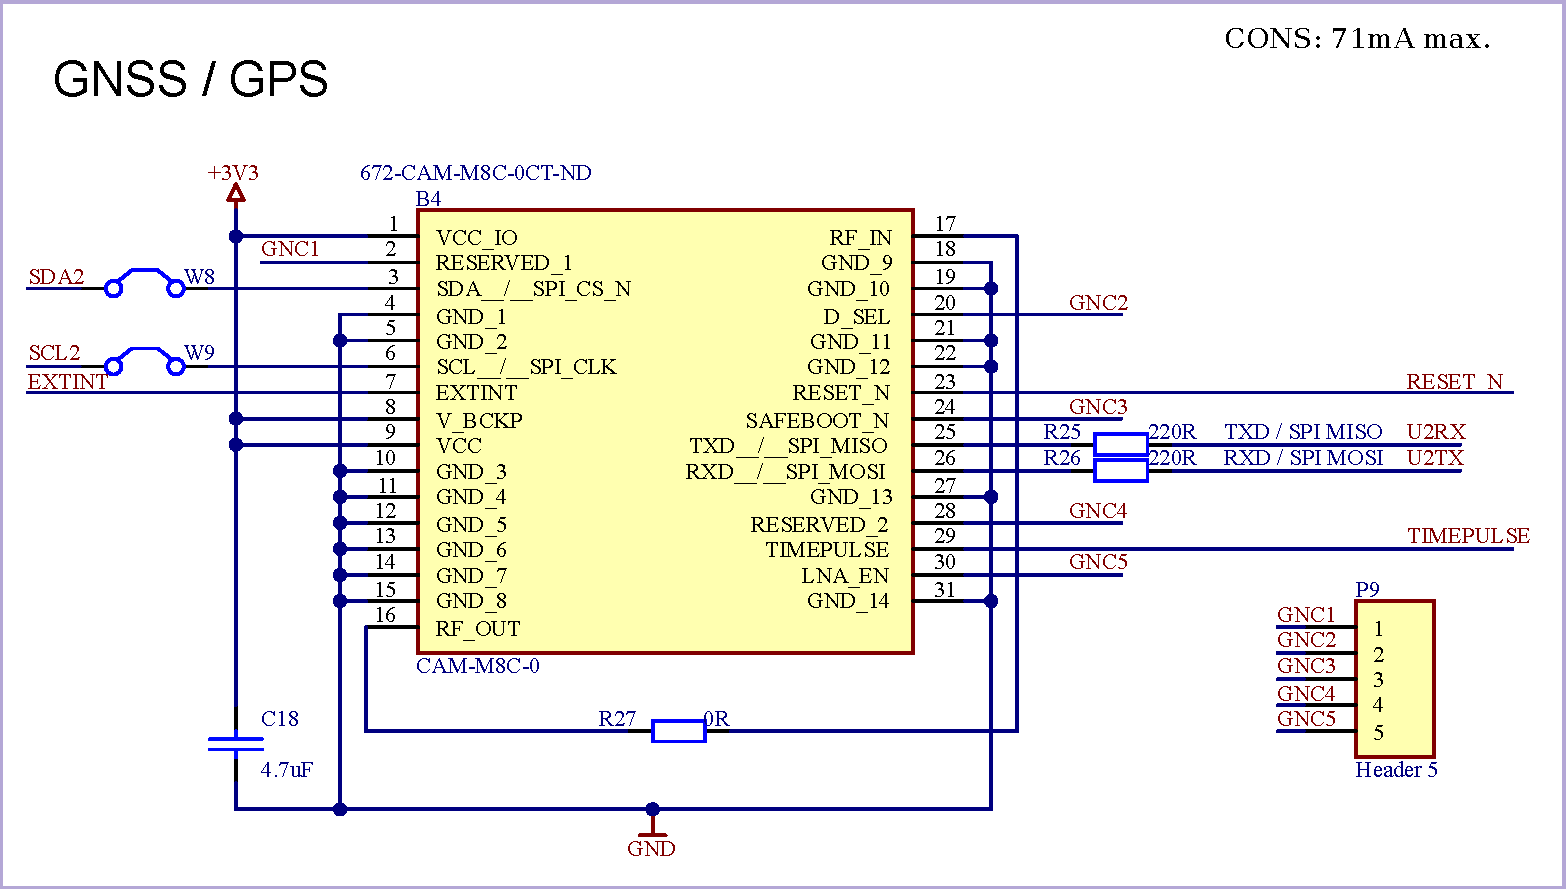
\includegraphics[width=.9\linewidth]{../figures/etude/sch/GNSS}
		\caption{Schéma du GNSS.}
		\label{fig:gnss}
	\end{figure}
\end{frame}

\begin{frame}{Peripherals - USB-FTDI}
	\begin{figure}[h]
		\centering
		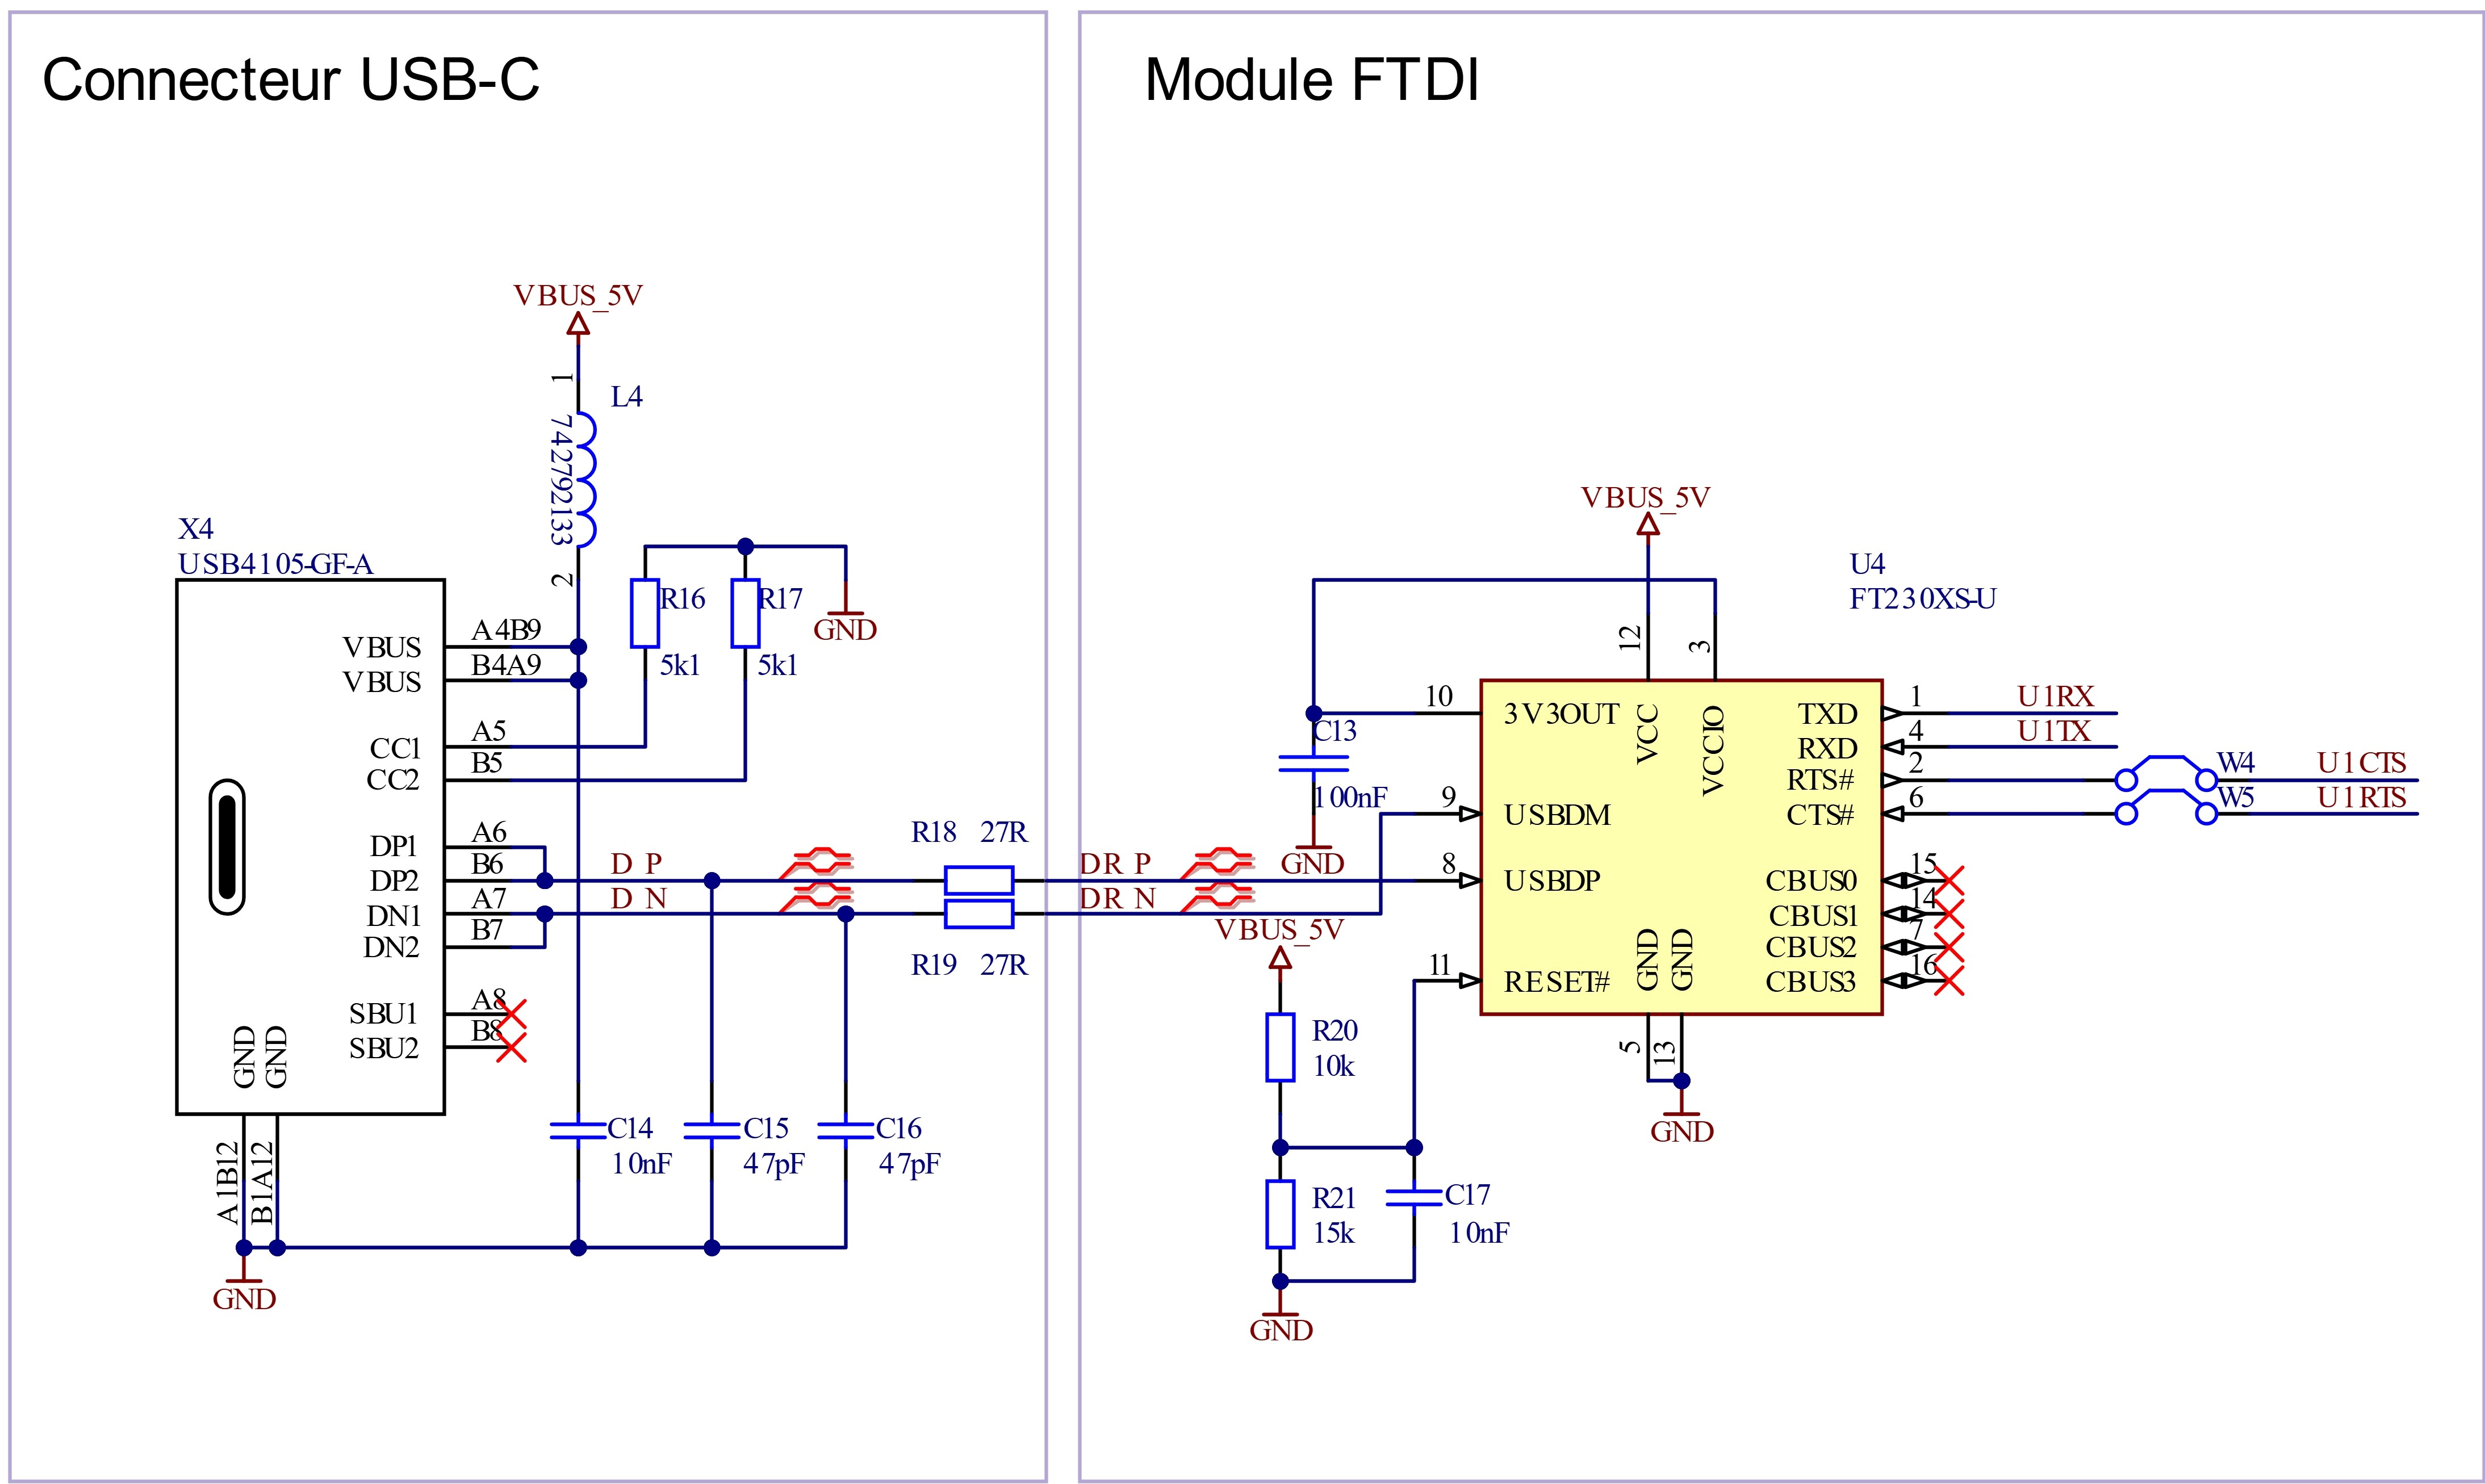
\includegraphics[width=.9\linewidth]{../figures/etude/sch/USB-FTDI}
		\caption{Schéma connecteur USB et FTDI.}
		\label{fig:usb-ftdi}
	\end{figure}
\end{frame}

\begin{frame}{Power - Chargeur de batterie}
	\begin{figure}[h]
		\centering
		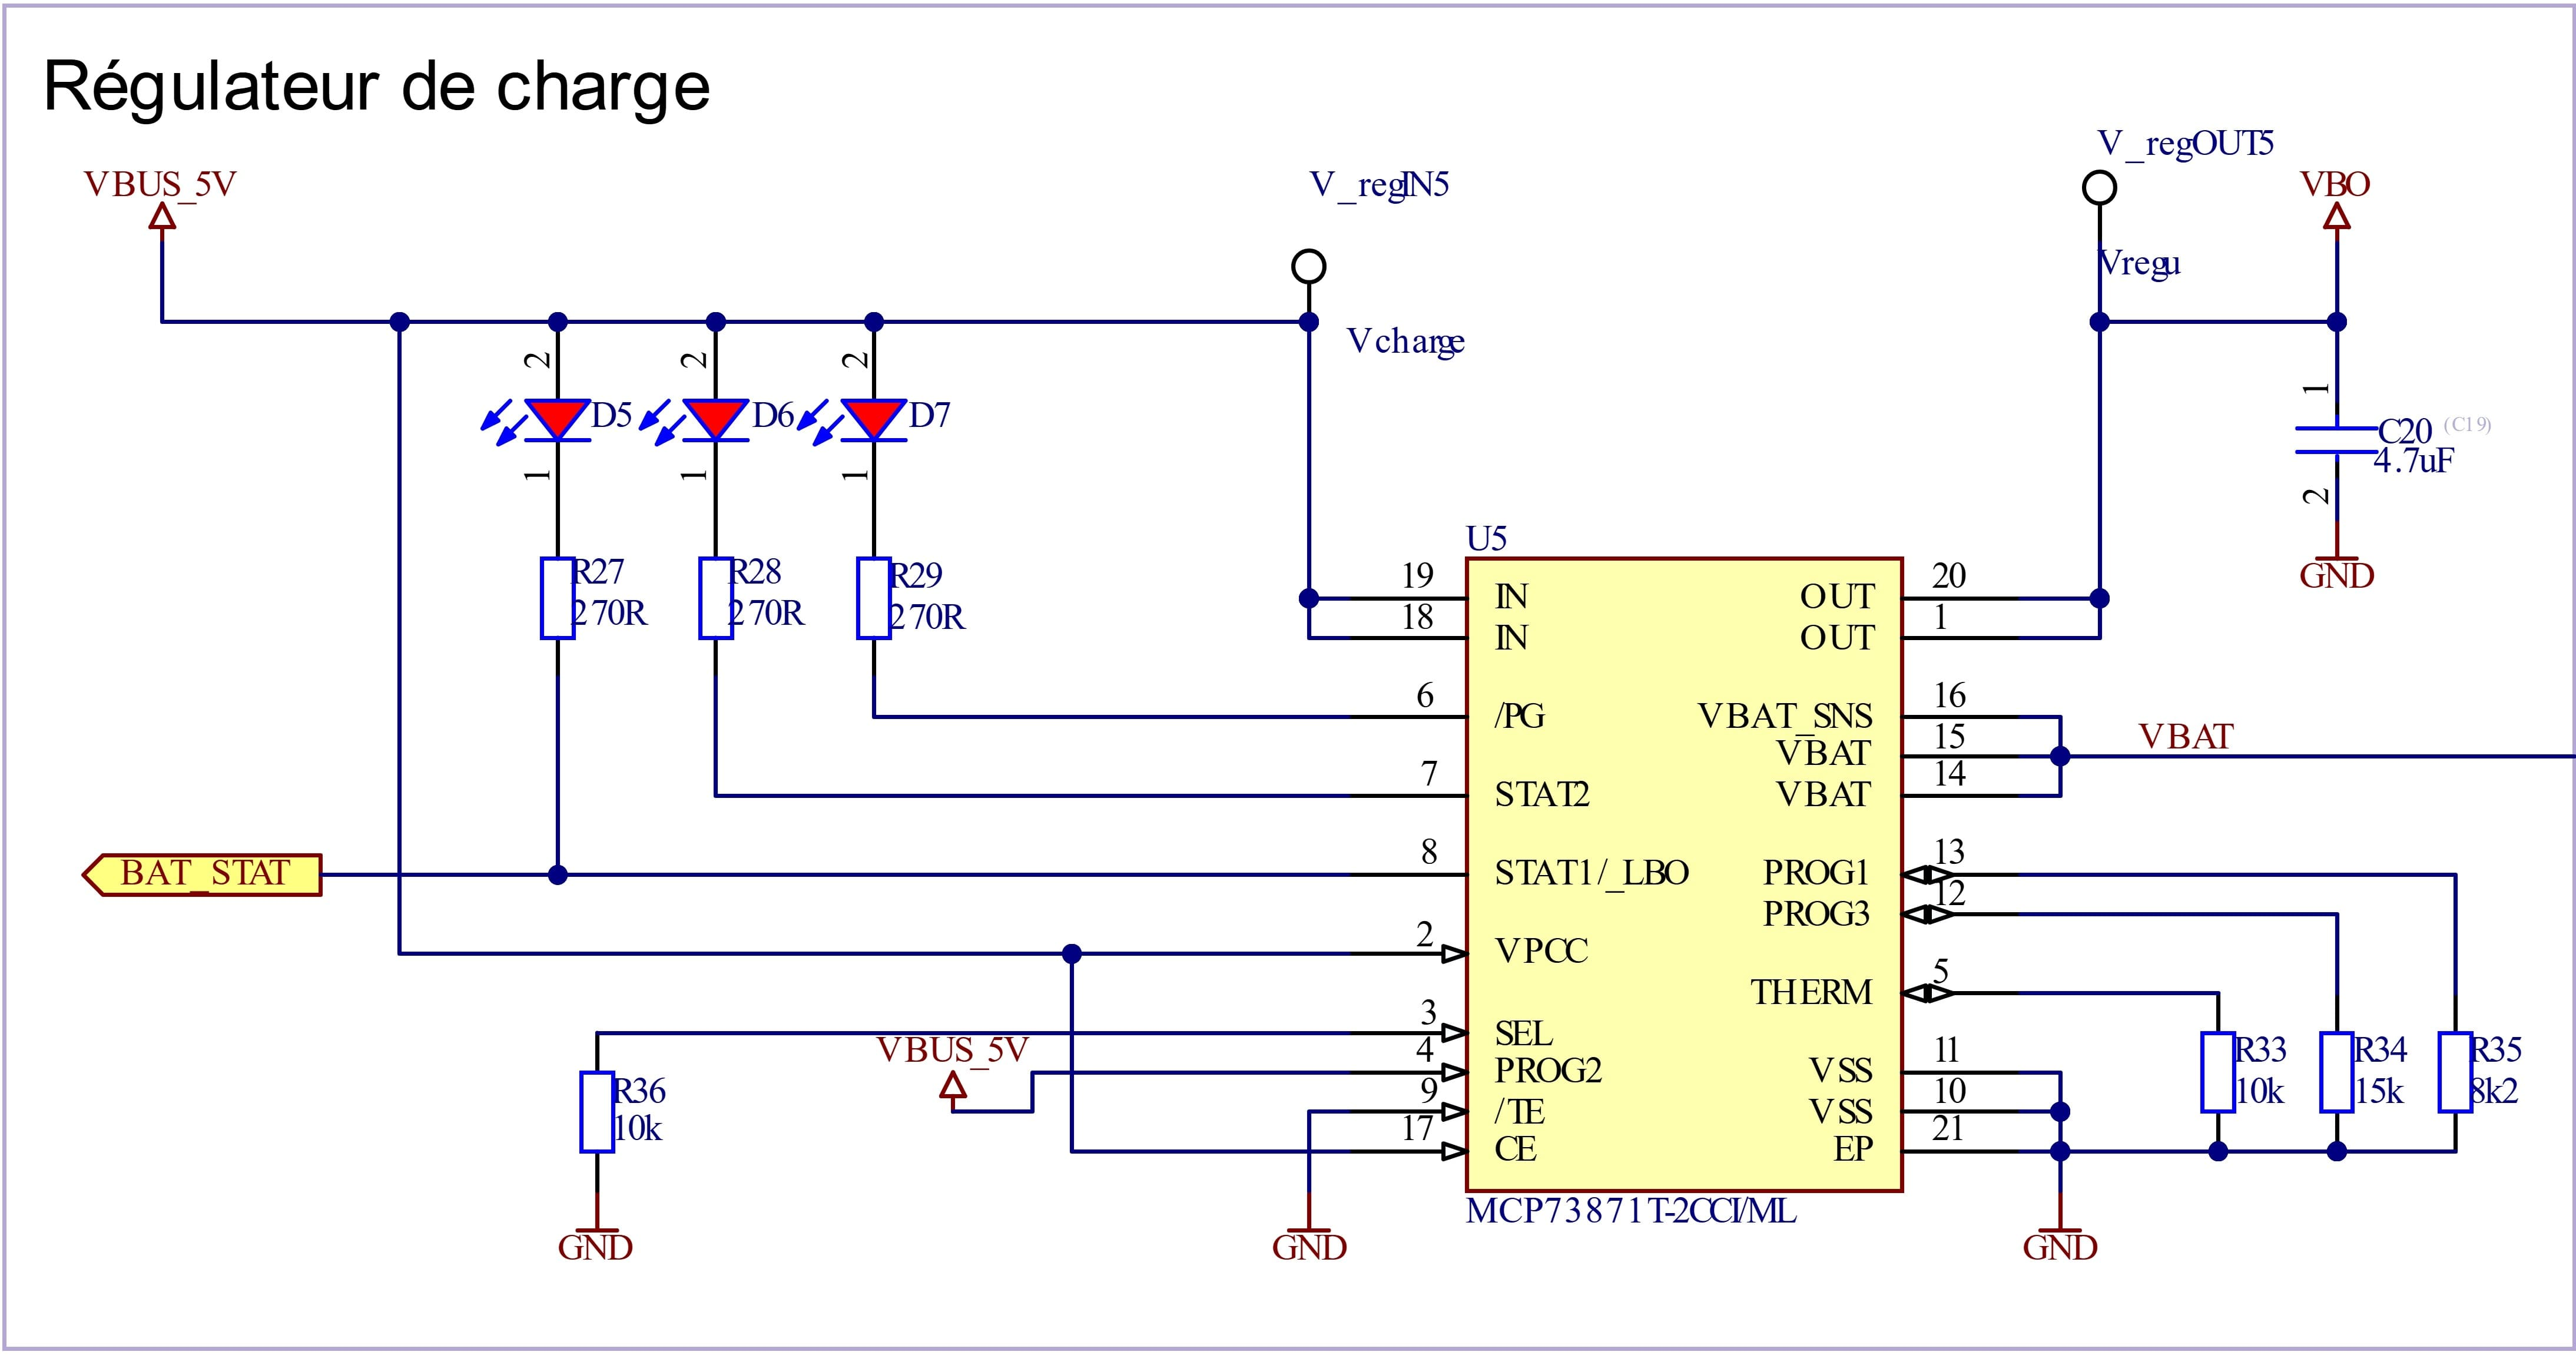
\includegraphics[width=.9\linewidth]{../figures/etude/sch/CHRG-BAT}
		\caption{Schéma chargeur de batterie.}
		\label{fig:chrg-bat}
	\end{figure}
\end{frame}

\begin{frame}{Power - Enclenchement}
	\begin{figure}[h]
		\centering
		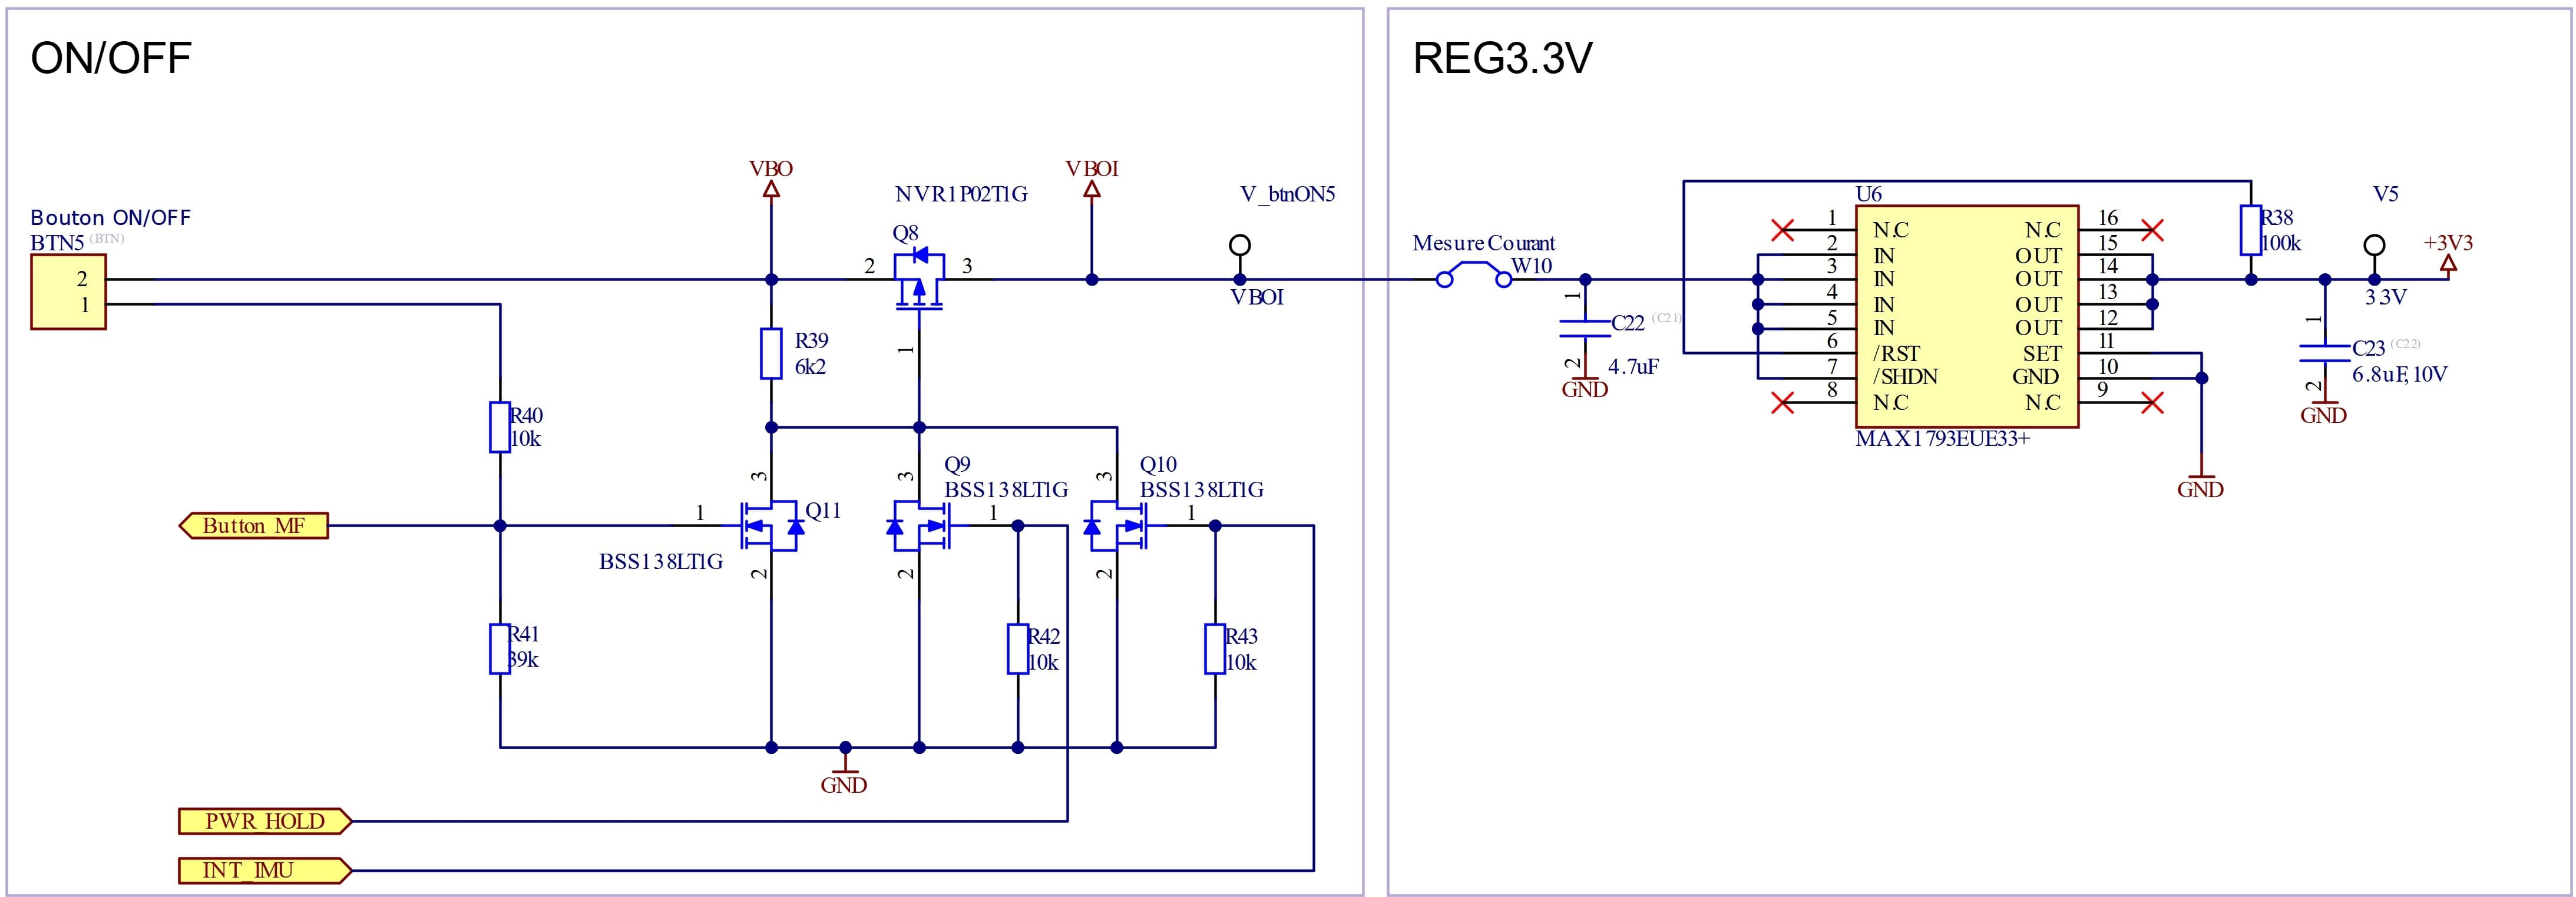
\includegraphics[width=1.07\linewidth]{../figures/etude/sch/ON-OFF}
		\caption{Schéma allumage du système.}
		\label{fig:on-off}
	\end{figure}
\end{frame}

\section{Développement du PCB}

\begin{frame}{Choix du boîtier}
	\begin{figure}[h]
		\centering
		\begin{subfigure}[b]{0.6\textwidth}
			\centering
			\includegraphics[width=\textwidth]{../figures/dev-pcb/boitier-dim}
		\end{subfigure}
		\hfill
		\begin{subfigure}[b]{0.35\textwidth}
			\centering
			\includegraphics[width=\textwidth]{../figures/dev-pcb/boitier-dims-pcb}
		\end{subfigure}
		\caption{Dimensions du SIC5-9-3B TAKACHI.}
	\end{figure}
\end{frame}

\begin{frame}{Placement des composants}
	\begin{figure}[h]
		\centering
		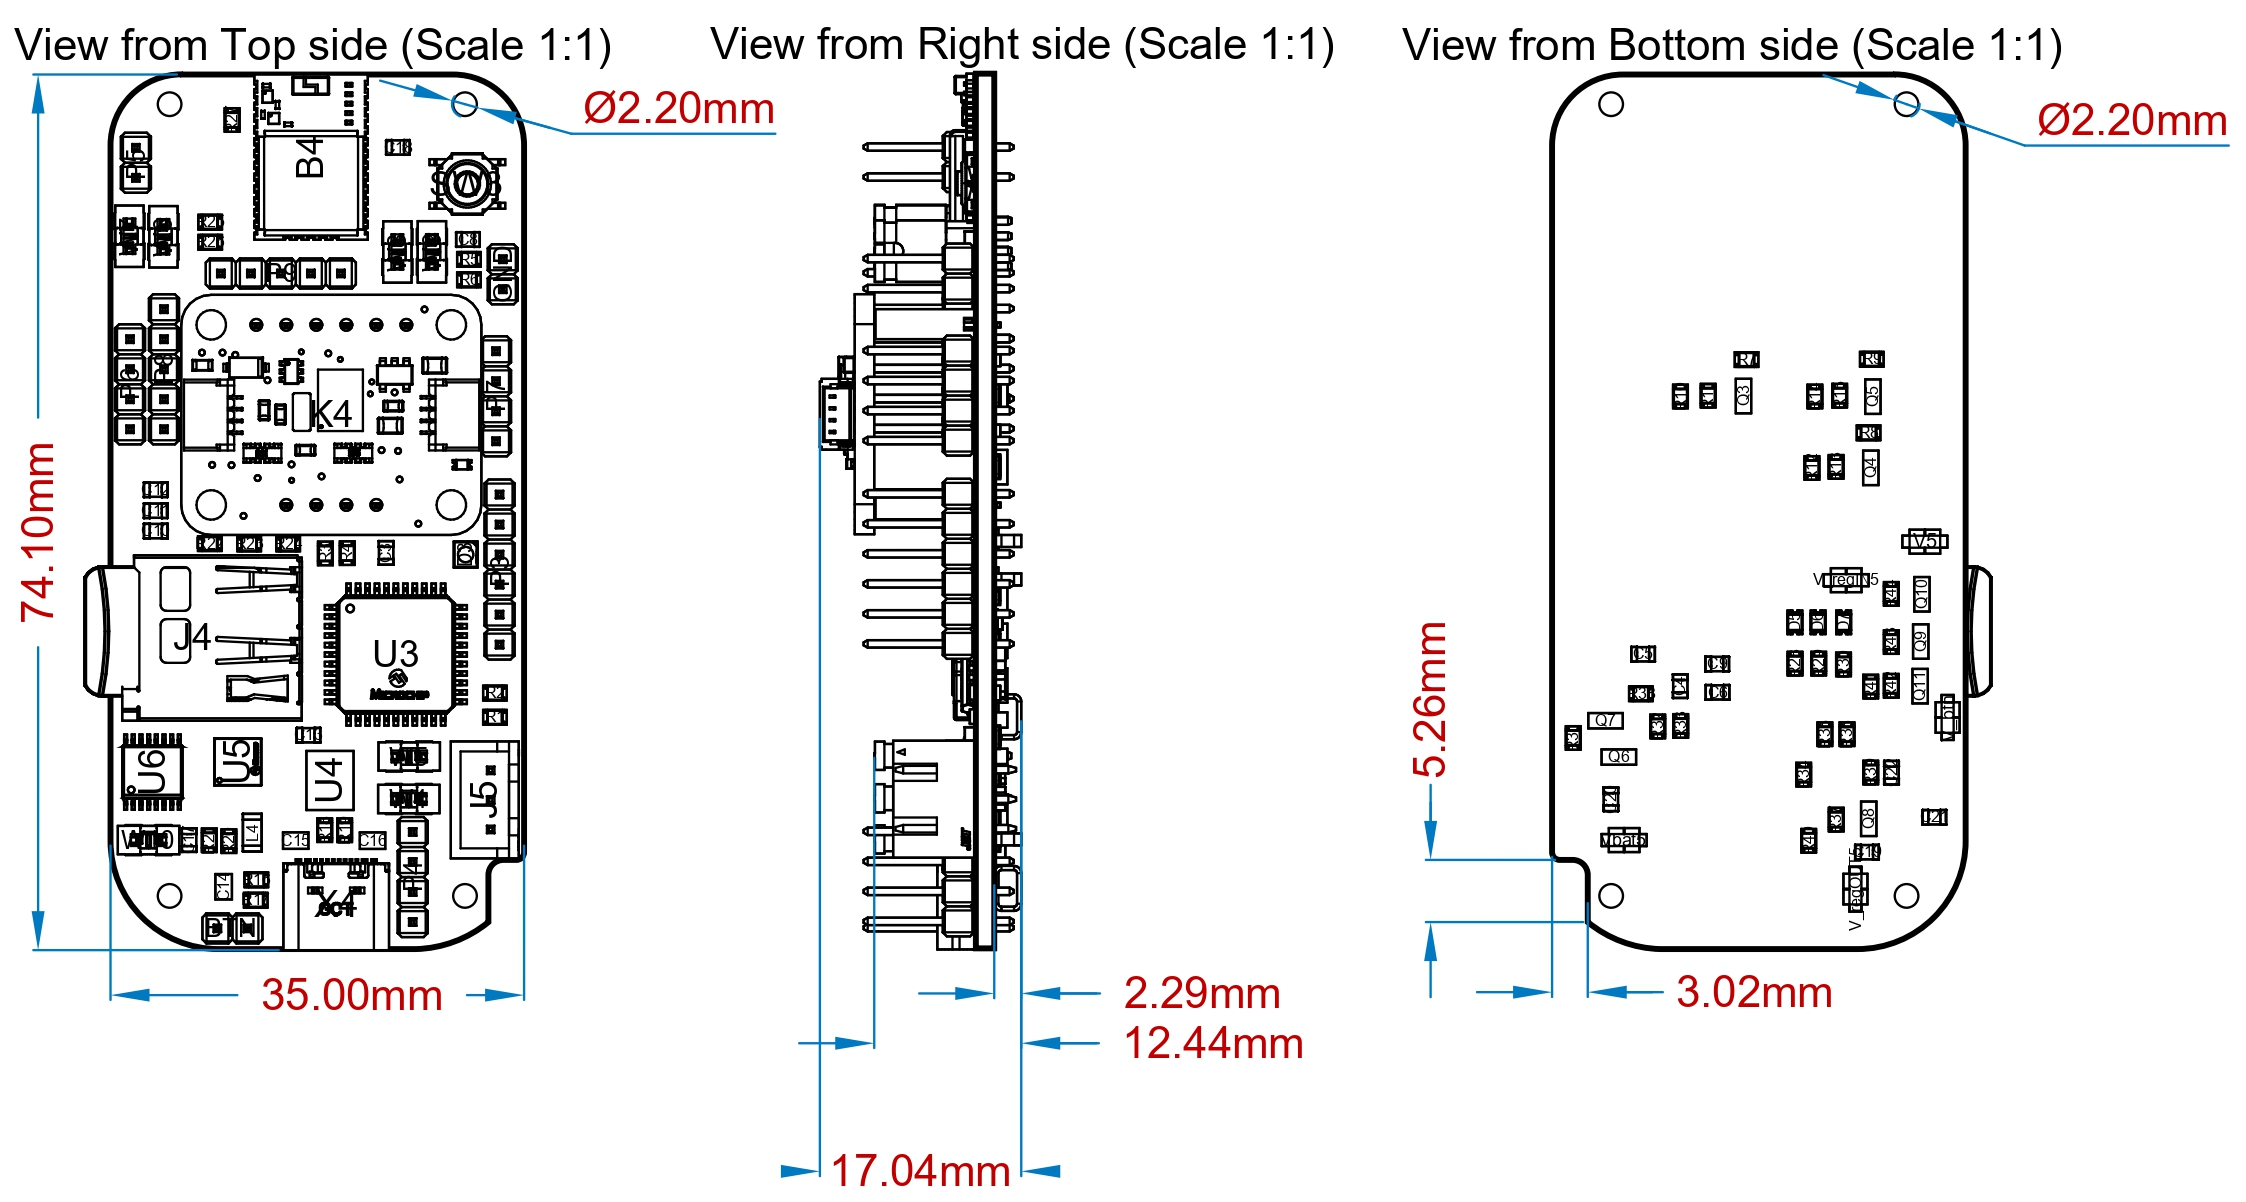
\includegraphics[width=.83\linewidth]{../figures/dev-pcb/PCB-Dims.jpg}
		\caption{Placement des composant et dimensions de la carte.}
		\label{fig:pcb-dims}
	\end{figure}
\end{frame}

\begin{frame}{Intégration}
	\begin{figure}[!h]
		\centering
		\begin{subfigure}[b]{0.24\textwidth}
			\centering
			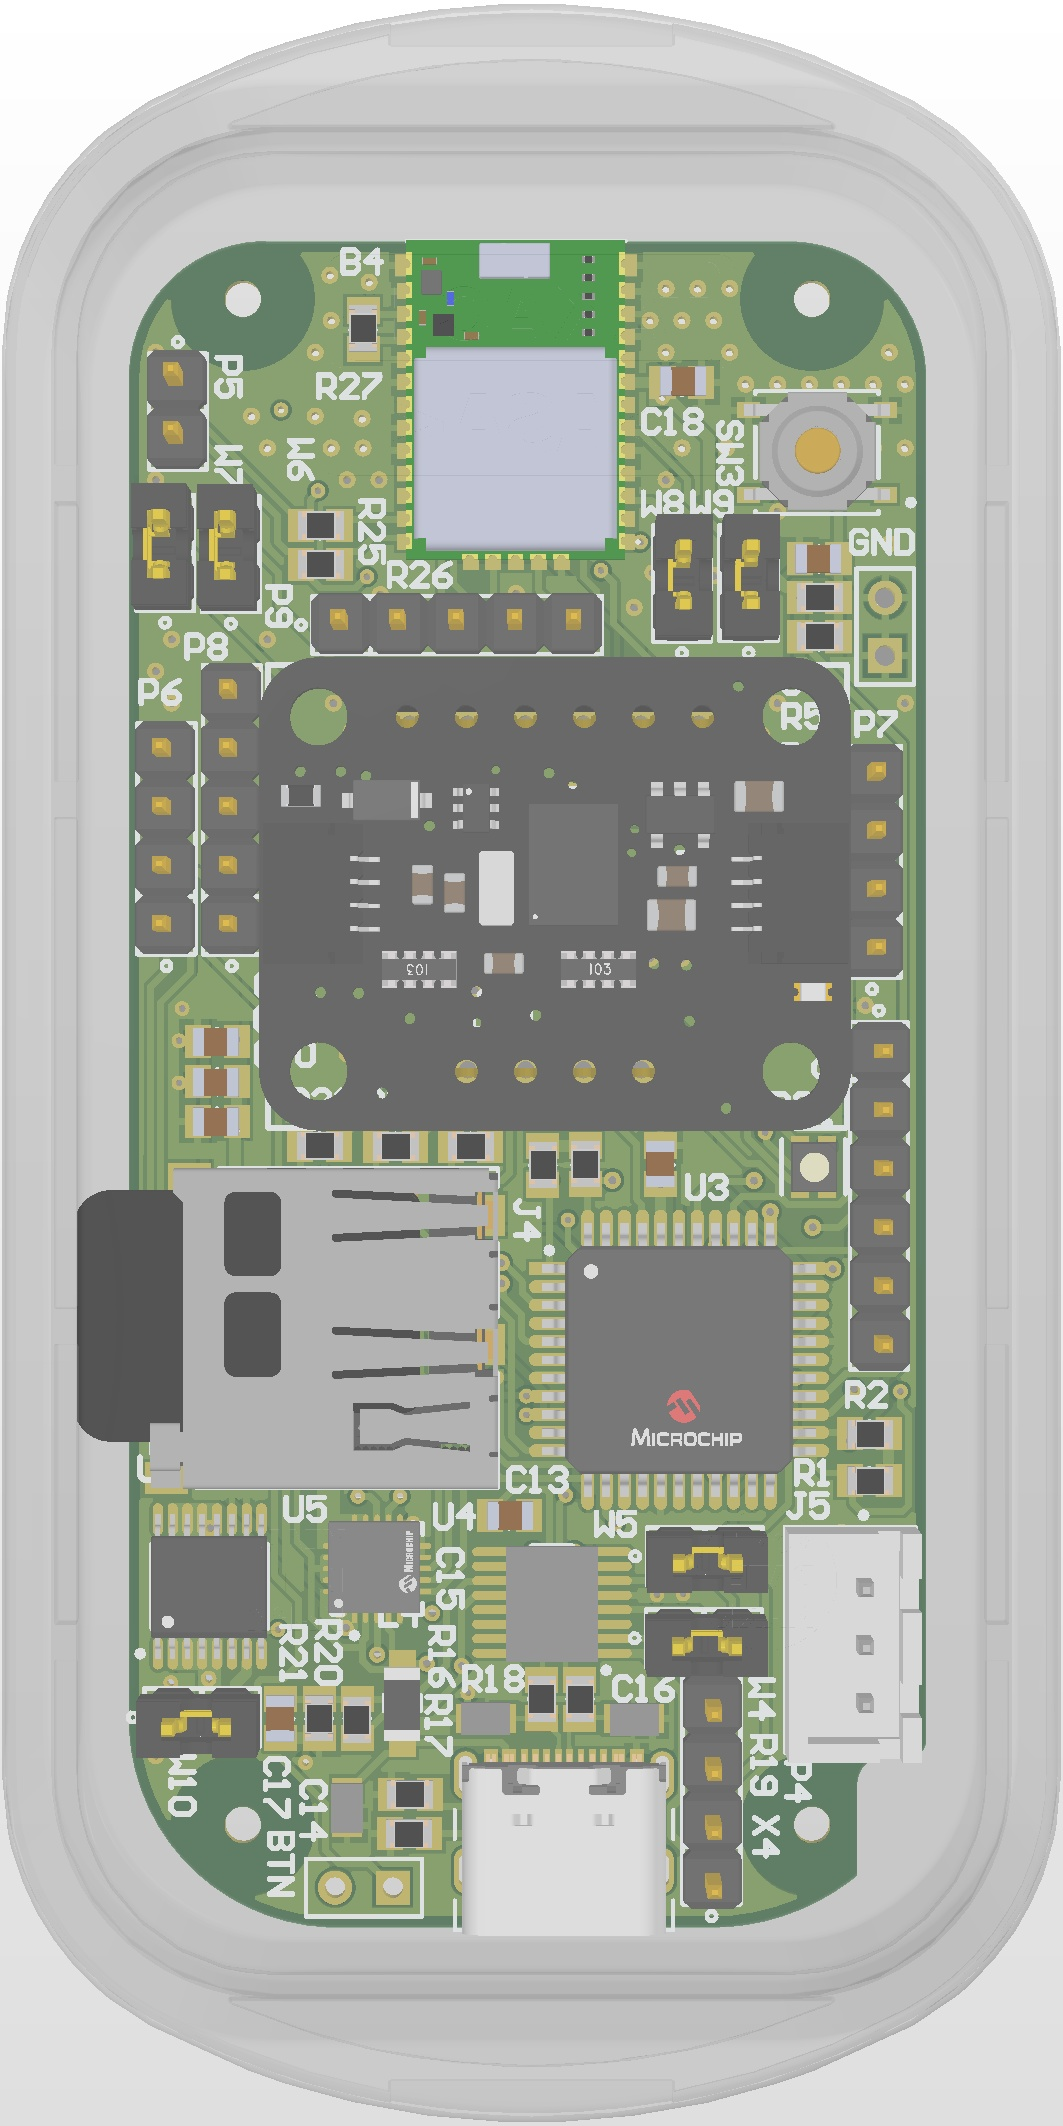
\includegraphics[width=\textwidth]{../figures/dev-pcb/3d-view3}
			\caption{Vue 3D, 1}
			\label{fig:3d-1}
		\end{subfigure}
		\hfill
		\begin{subfigure}[b]{0.33\textwidth}
			\centering
			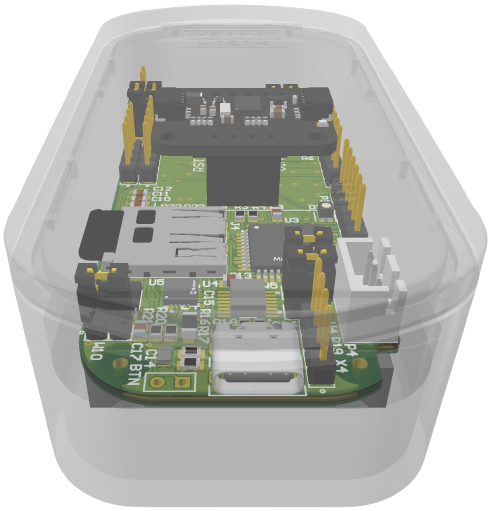
\includegraphics[width=\textwidth]{../figures/dev-pcb/3d-view2}
			\caption{Vue 3D, 2}
			\label{fig:3d-2}
		\end{subfigure}
		\hfill
		\begin{subfigure}[b]{0.36\textwidth}
			\centering
			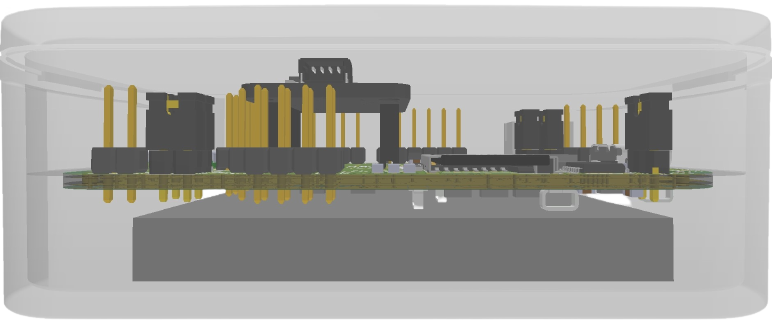
\includegraphics[width=\textwidth]{../figures/dev-pcb/3d-view1}
			\caption{Vue 3D, 3}
			\label{fig:3d-3}
		\end{subfigure}
		\caption{Vues 3d de l'assemblage.}
		\label{fig:MechAssembly}
	\end{figure}
\end{frame}

\begin{frame}{Routage}
	\begin{figure}[!h]
		\centering
		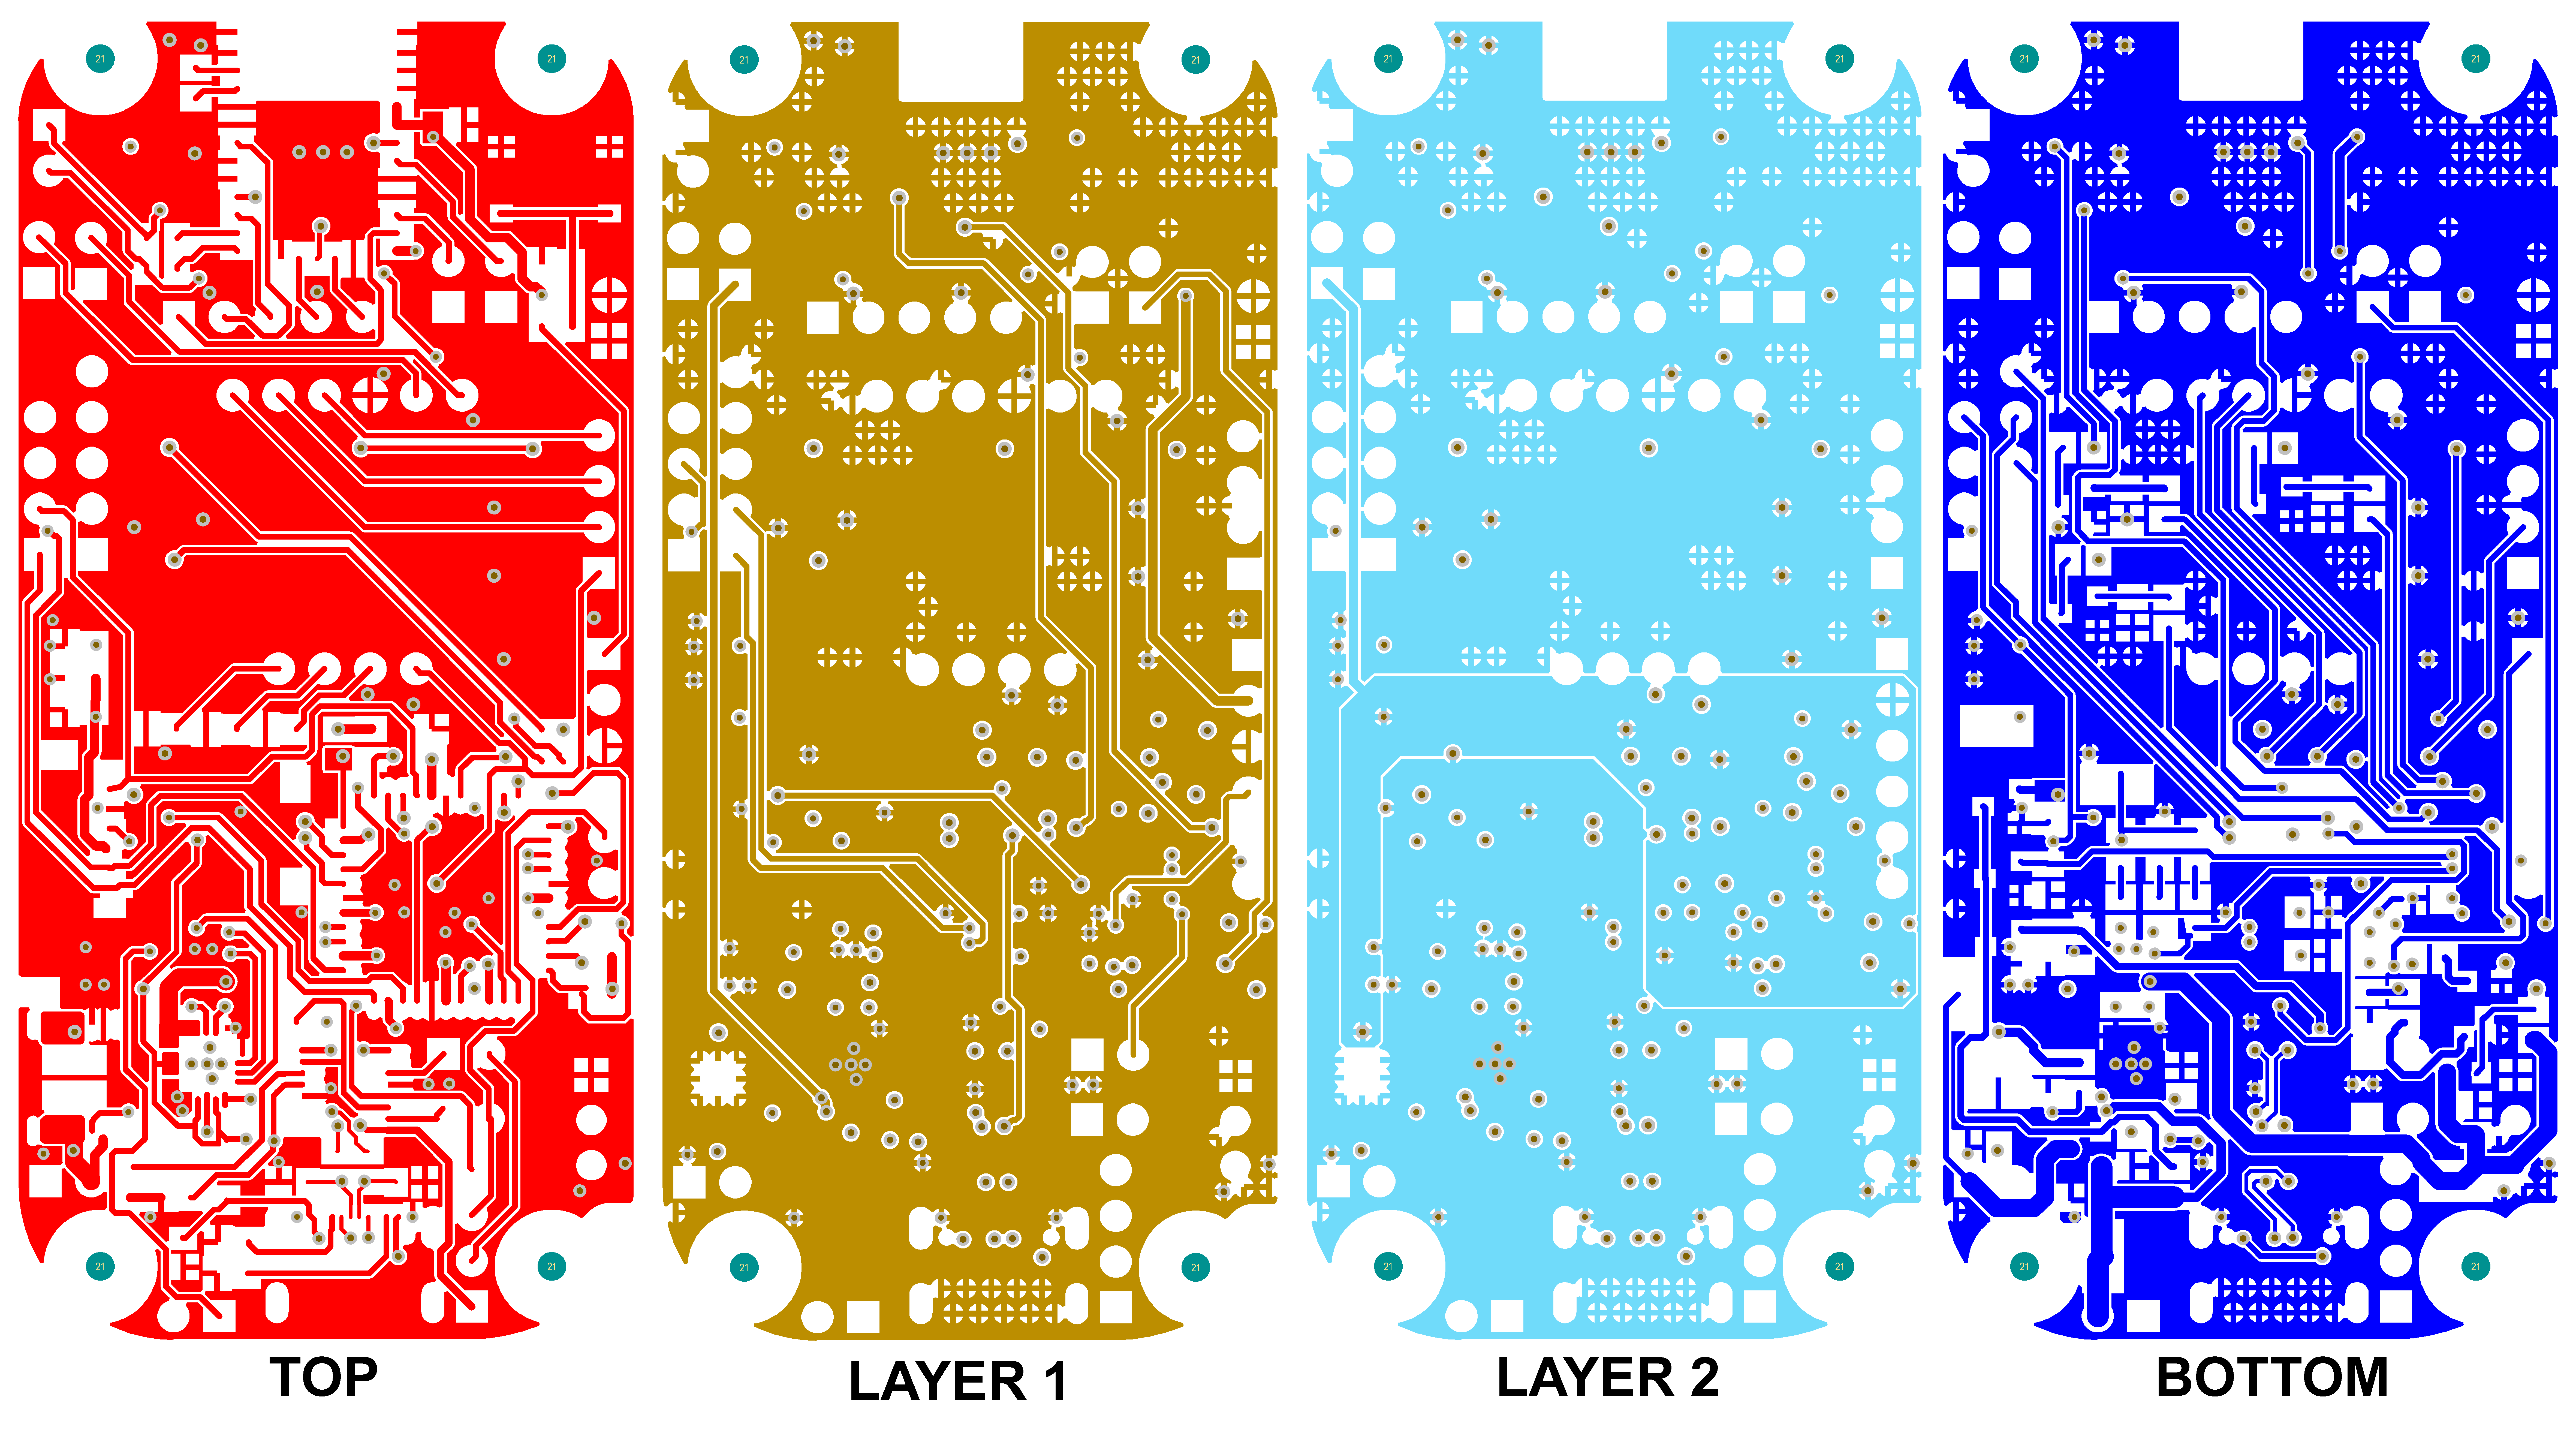
\includegraphics[width=.9\linewidth]{../figures/dev-pcb/Couches-layout}
		\caption{Routage des différentes couches.}
		\label{fig:couches-layout}
	\end{figure}
\end{frame}

\section{Développement du firmware}


\begin{frame}{Configuration des périphériques}
	\begin{table}[h]
		\resizebox{1\textwidth}{!}{\begin{tabular}{lll}
			ID du timer & Description & Période \\
			\hline
			\textbf{Timer 1} & sert pour les attentes bloquantes précises. & 1 [$ms$] \\
			\textbf{Timer 2} & gère les délais entre les mesures et l'affichage des LEDs. & 10 [$ms$] \\
		\end{tabular}}
	\end{table}
	
	\begin{center}
		\begin{table}[h]
			\centering
			\resizebox{1\textwidth}{!}{\begin{tabular}{llllll}
				ID du BUS & Utilité & Fréquence & Interruption & Trame & Parité \\ 
				\hline
				\textbf{UART ID1} & Réceptions commandes USB. & 9600 [Baud] & Priorité 1 & 8bits + 1stop & Non \\
				\textbf{UART ID2} & Communication avec le GNSS. & 9600 [Baud] & Non & 8bits + 1stop & Non \\
				\textbf{SPI} & Communication avec la carte SD en FAT32. & 12'000 [MHz] & Priorité 1 & - & - \\
				\textbf{I2C} & Communication avec la centrale inertielle. & 400 [kbit/s] & & & \\
			\end{tabular}}
			\caption{}
			\label{tab:Usarts}
		\end{table}
	\end{center}
\end{frame}

%\begin{frame}{Messages NMEA}
%	\begin{figure}[h]
%		\centering
%		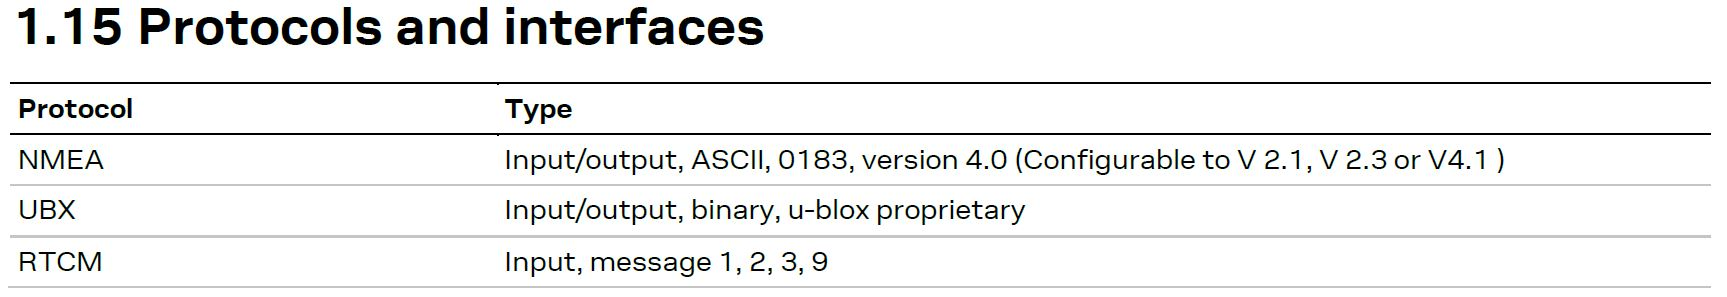
\includegraphics[width=.8\linewidth]{../figures/code/Protocols}
%		\caption{Protocoles disponibles.}
%		\label{fig:protocolsGNSS}
%	\end{figure} 
%	\begin{figure}[h]
%		\centering
%		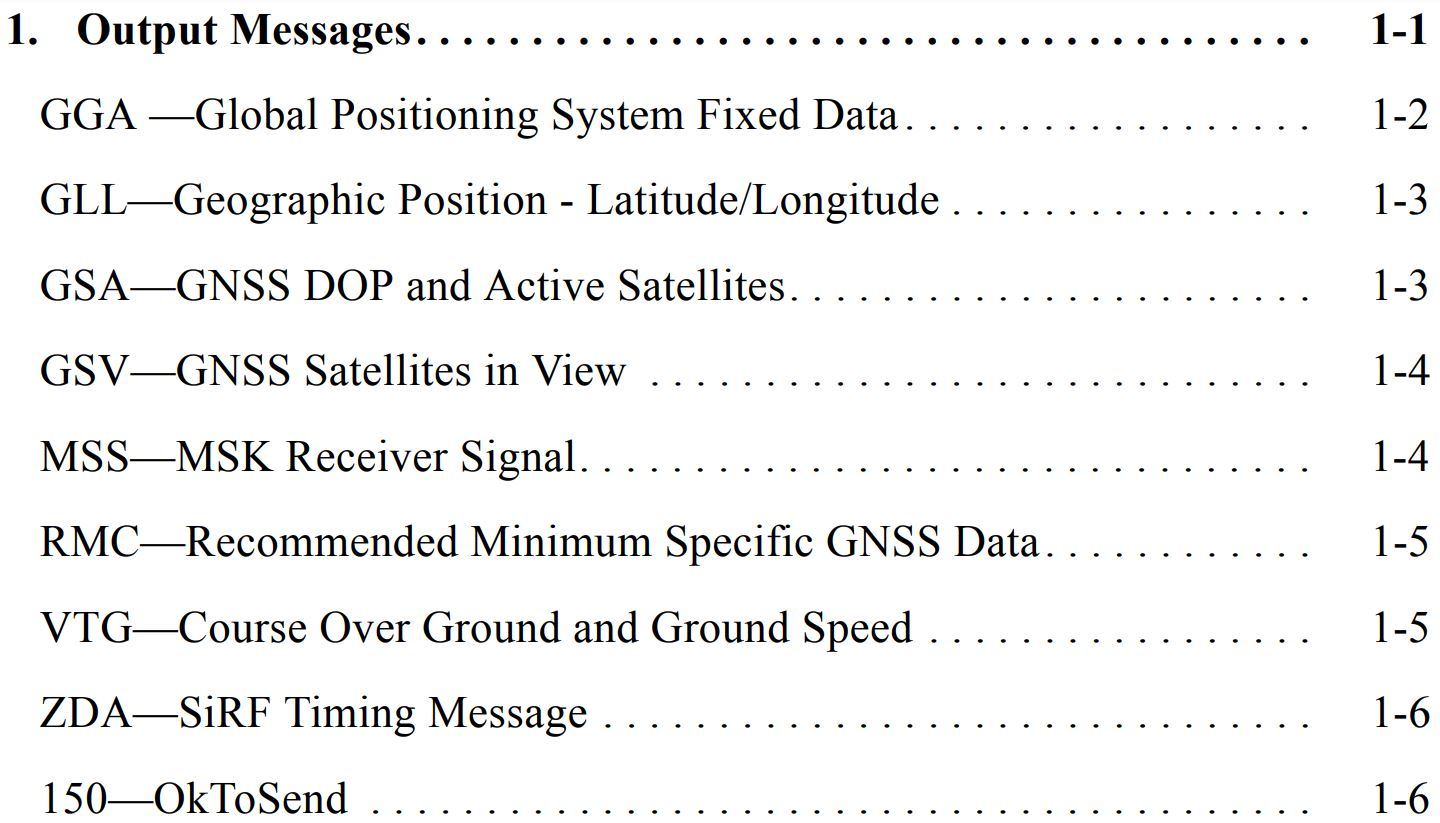
\includegraphics[width=0.7\linewidth]{../figures/code/Messages-NMEA}
%		\caption{Messages NMEA.}
%		\label{fig:messages-nmea}
%	\end{figure}
%\end{frame}

\begin{frame}{Diagramme application principale}
	\begin{figure}[h]
		\centering
		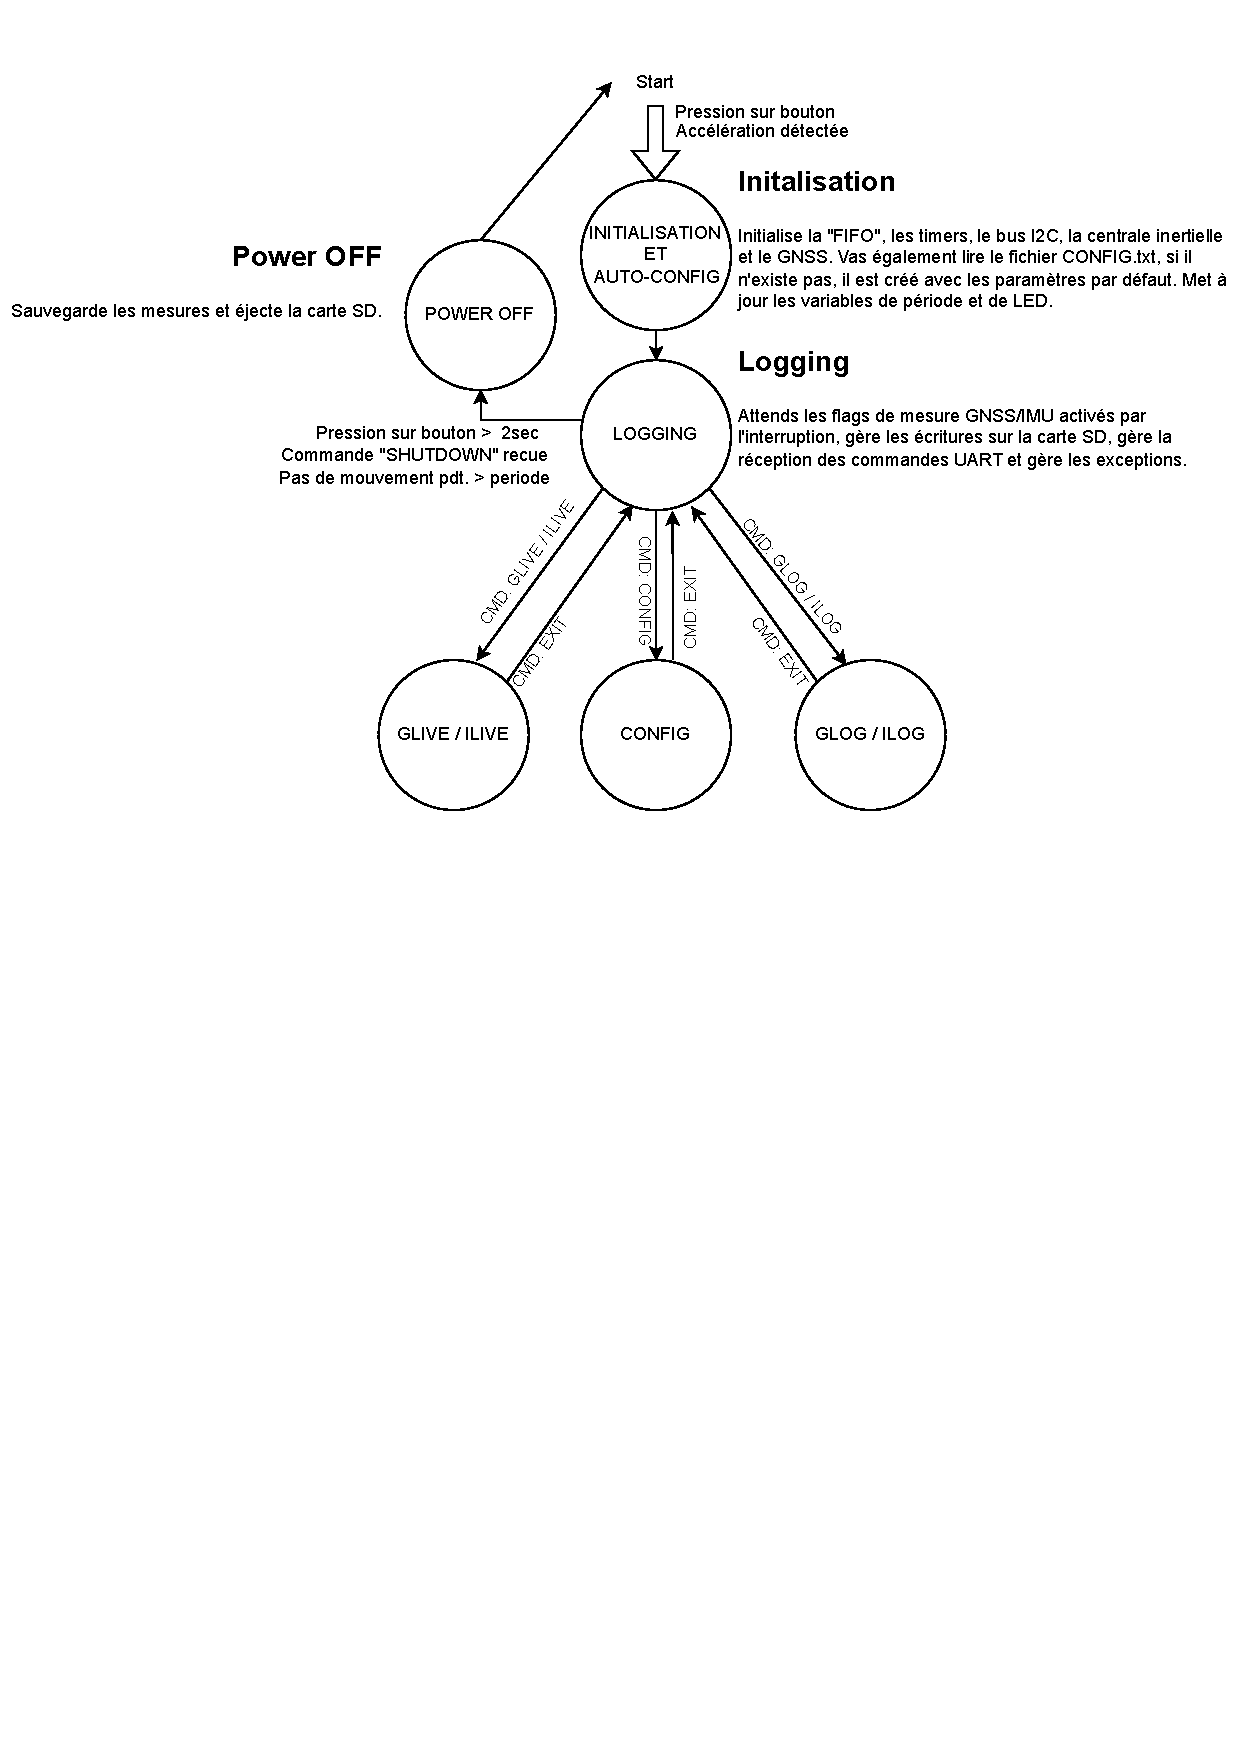
\includegraphics[width=1\linewidth]{../figures/code/diagrammes/state_app}
		\caption{Diagramme d'état principal.}
		\label{fig:stateapp}
	\end{figure}
\end{frame}

\begin{frame}{Diagramme de séquence principale}
	\begin{figure}[!h]
		\centering
		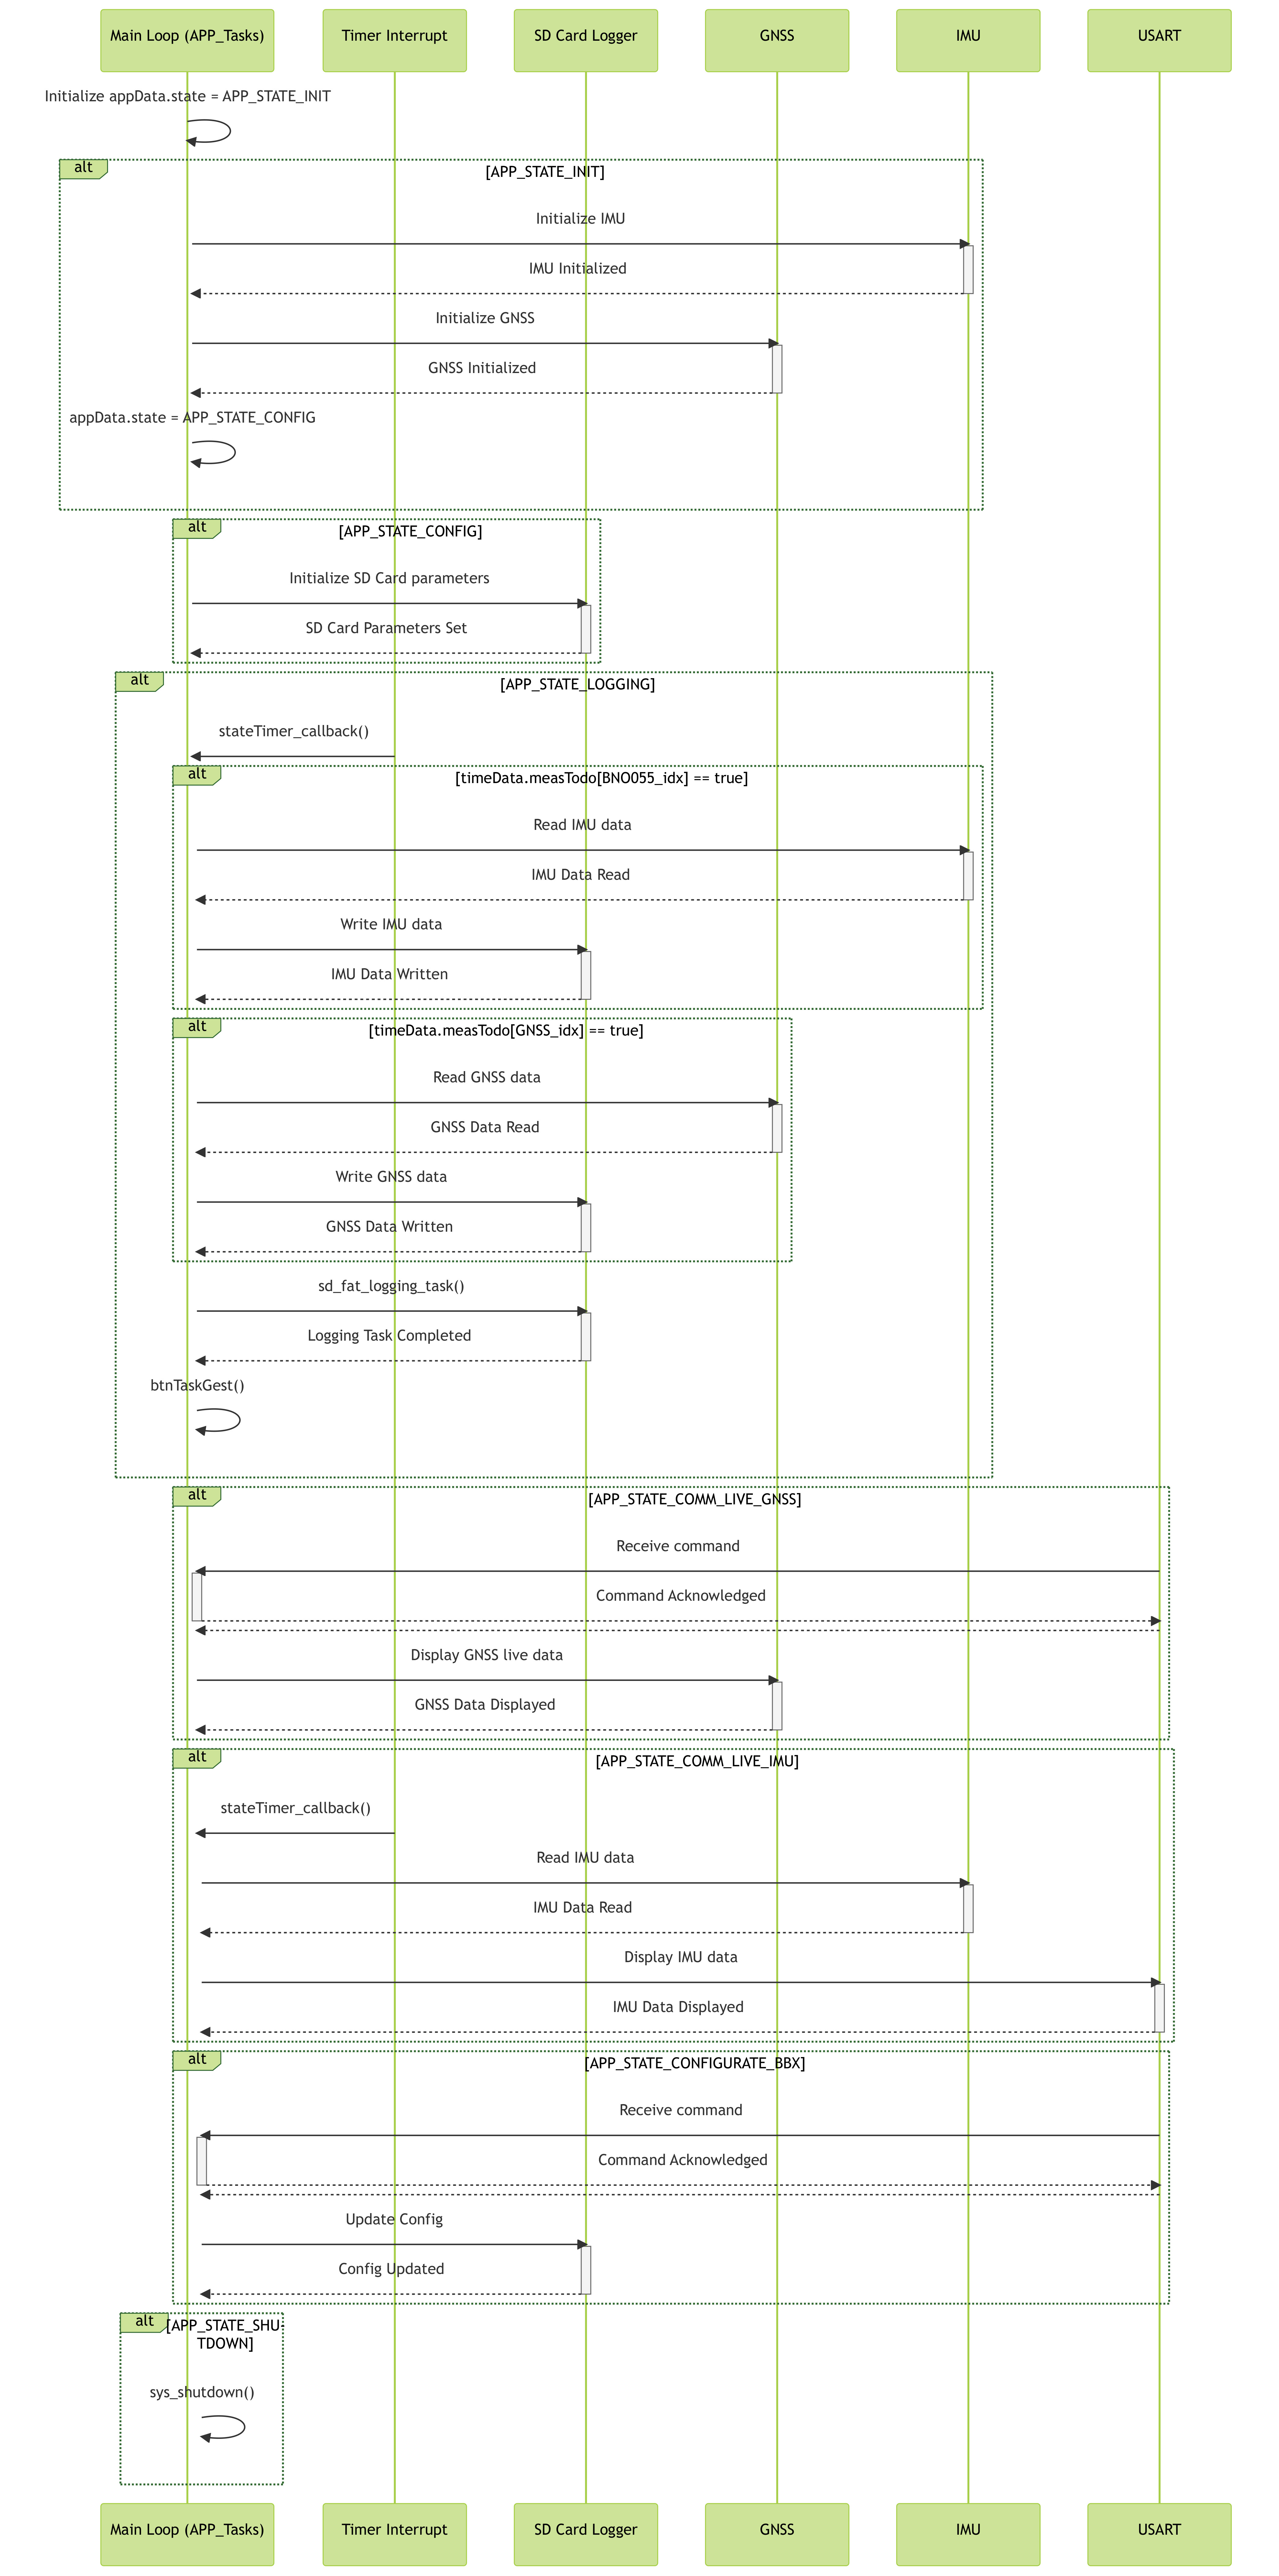
\includegraphics[height=.9\textheight]{../figures/code/diagrammes/sequence-app}
		\label{fig:sequence-app}
	\end{figure}
\end{frame}

\begin{frame}{Flowchart Logging}
	\begin{figure}[!h]
		\centering
		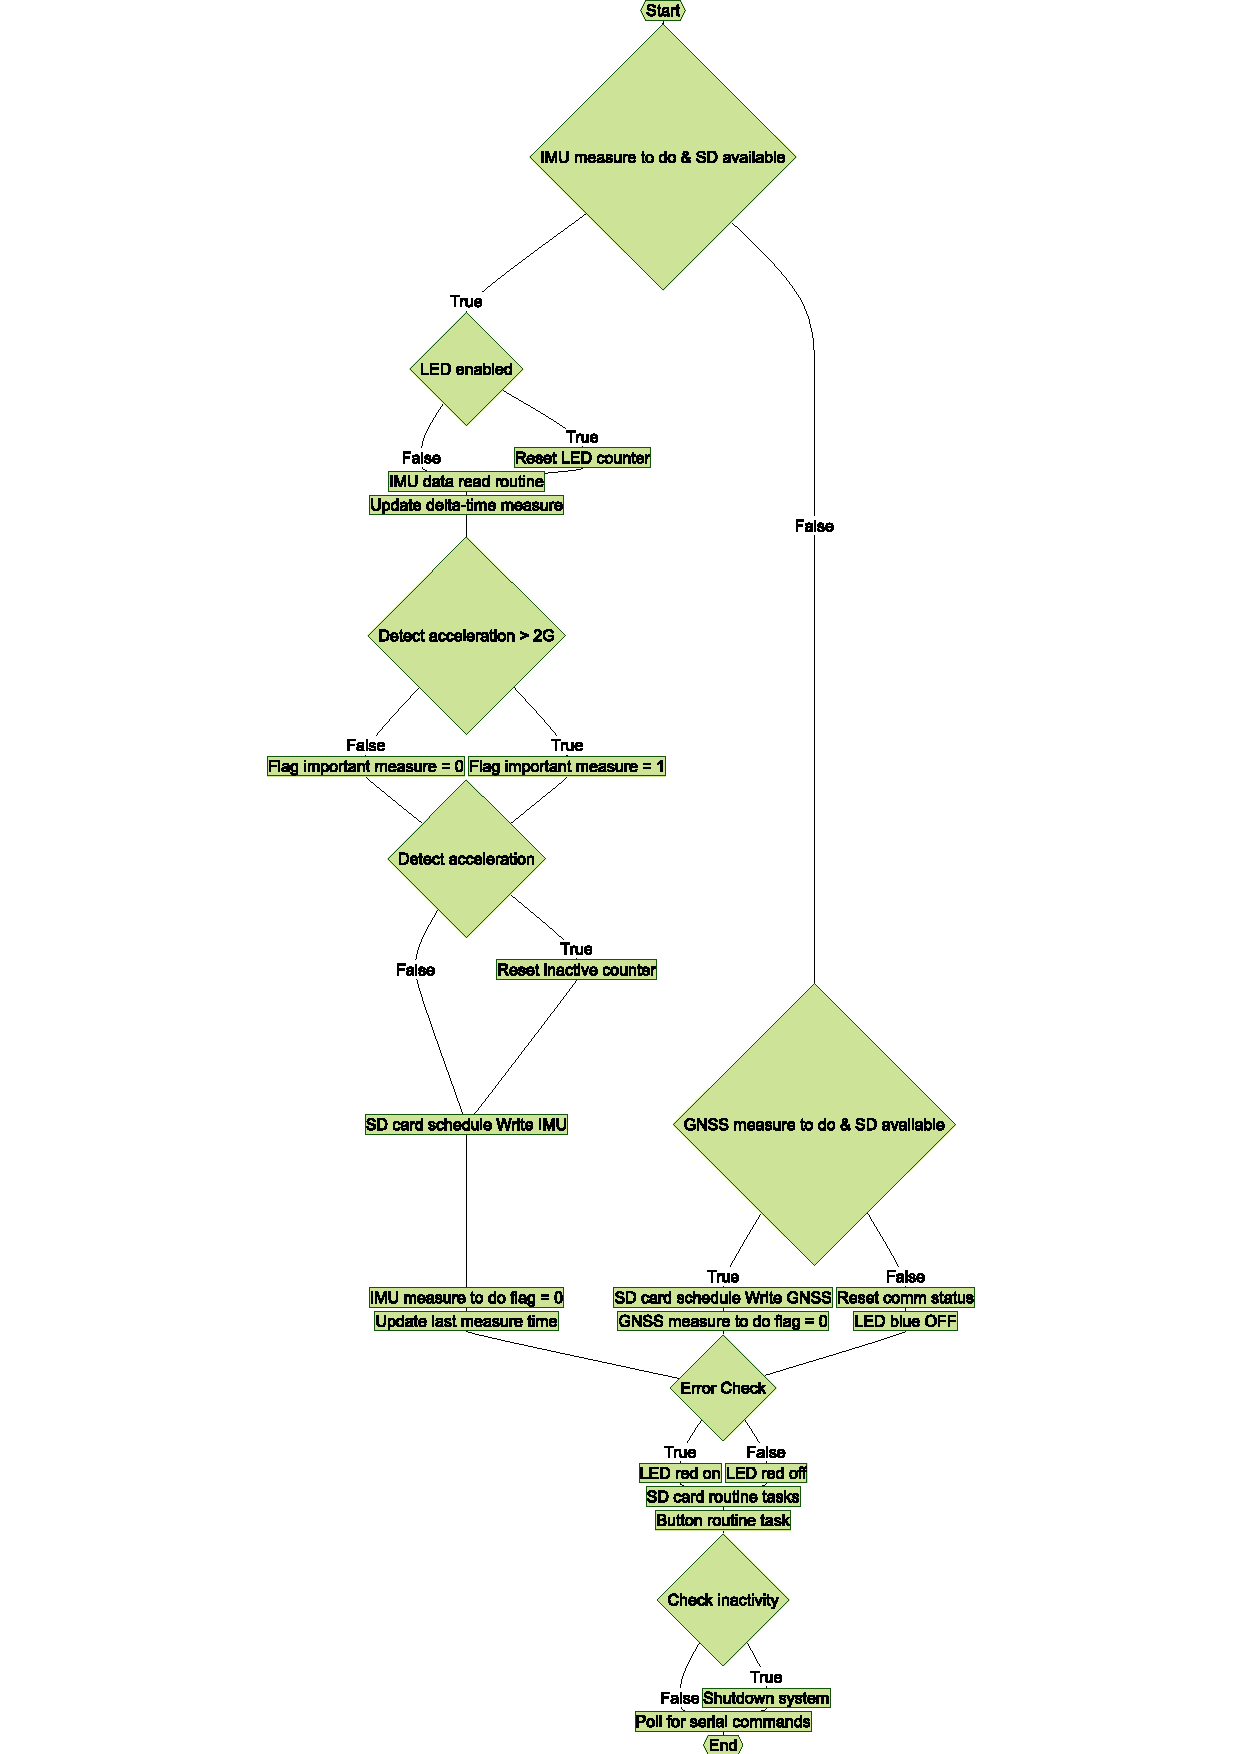
\includegraphics[height=.9\textheight]{../figures/code/diagrammes/logging-flowchart}
		\label{fig:pdfresizer}
	\end{figure}
\end{frame}

\begin{frame}{Carte SD}
	\begin{figure}[h]
		\centering
		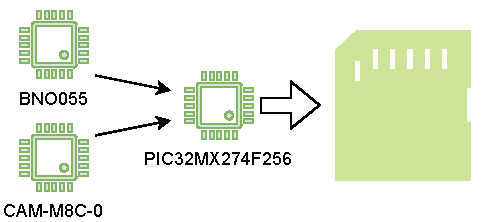
\includegraphics[width=0.6\linewidth]{../figures/code/Illustration-SD-per}
		\label{fig:illustration-sd-per}
	\end{figure}
\end{frame}

\begin{frame}{Machine d'état carte SD - Initialisation}
	\begin{figure}[h]
		\centering
		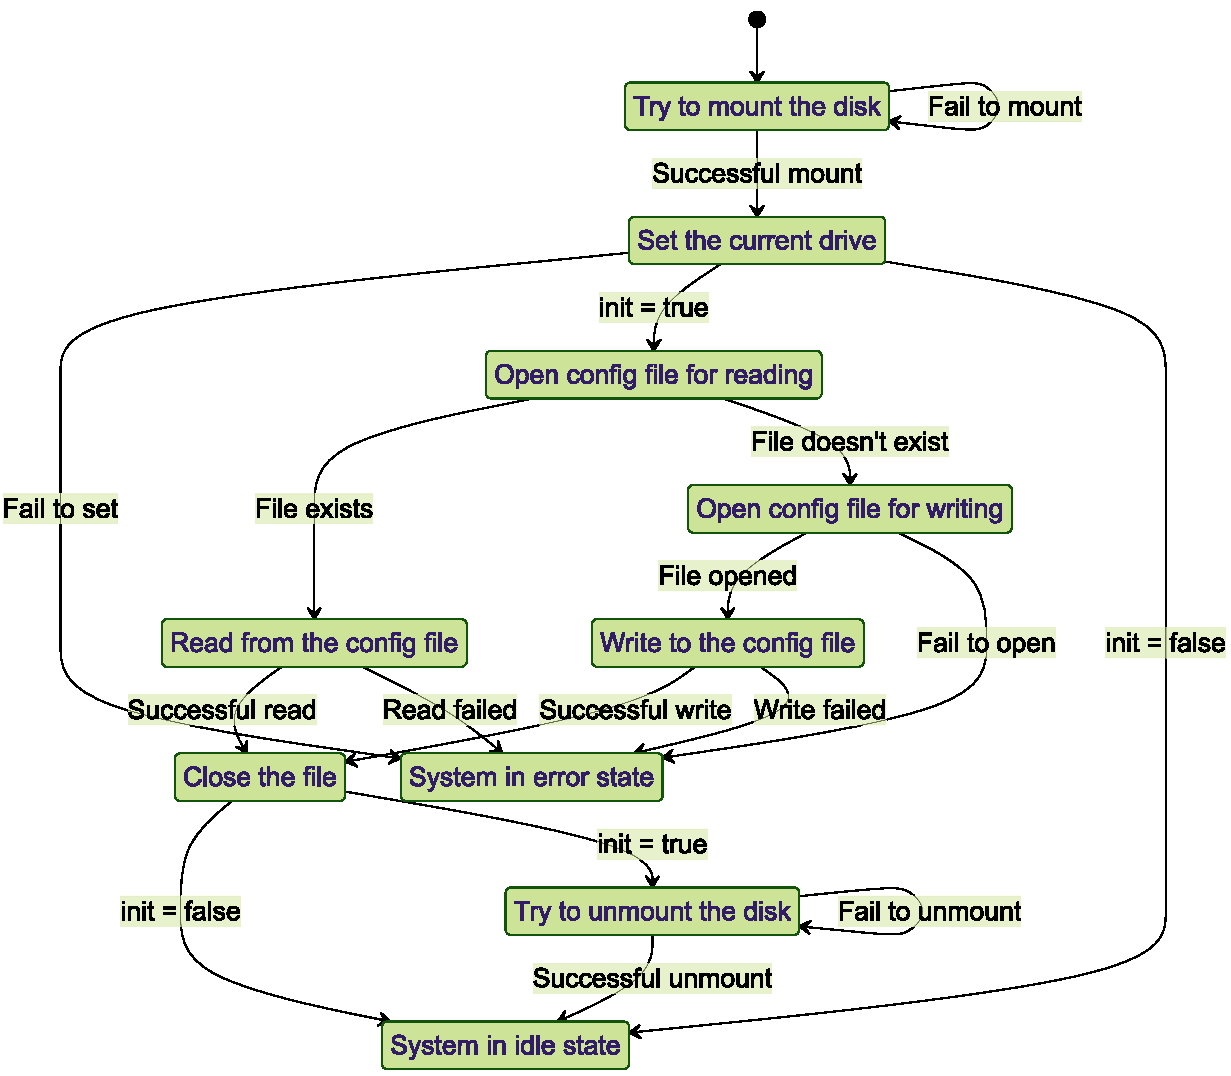
\includegraphics[height=.9\textheight]{../figures/code/diagrammes/sd-card-Init}
		\label{fig:sd-card-init}
	\end{figure}
\end{frame}

\begin{frame}{Machine d'état carte SD - Logging}
\begin{figure}[h]
	\centering
	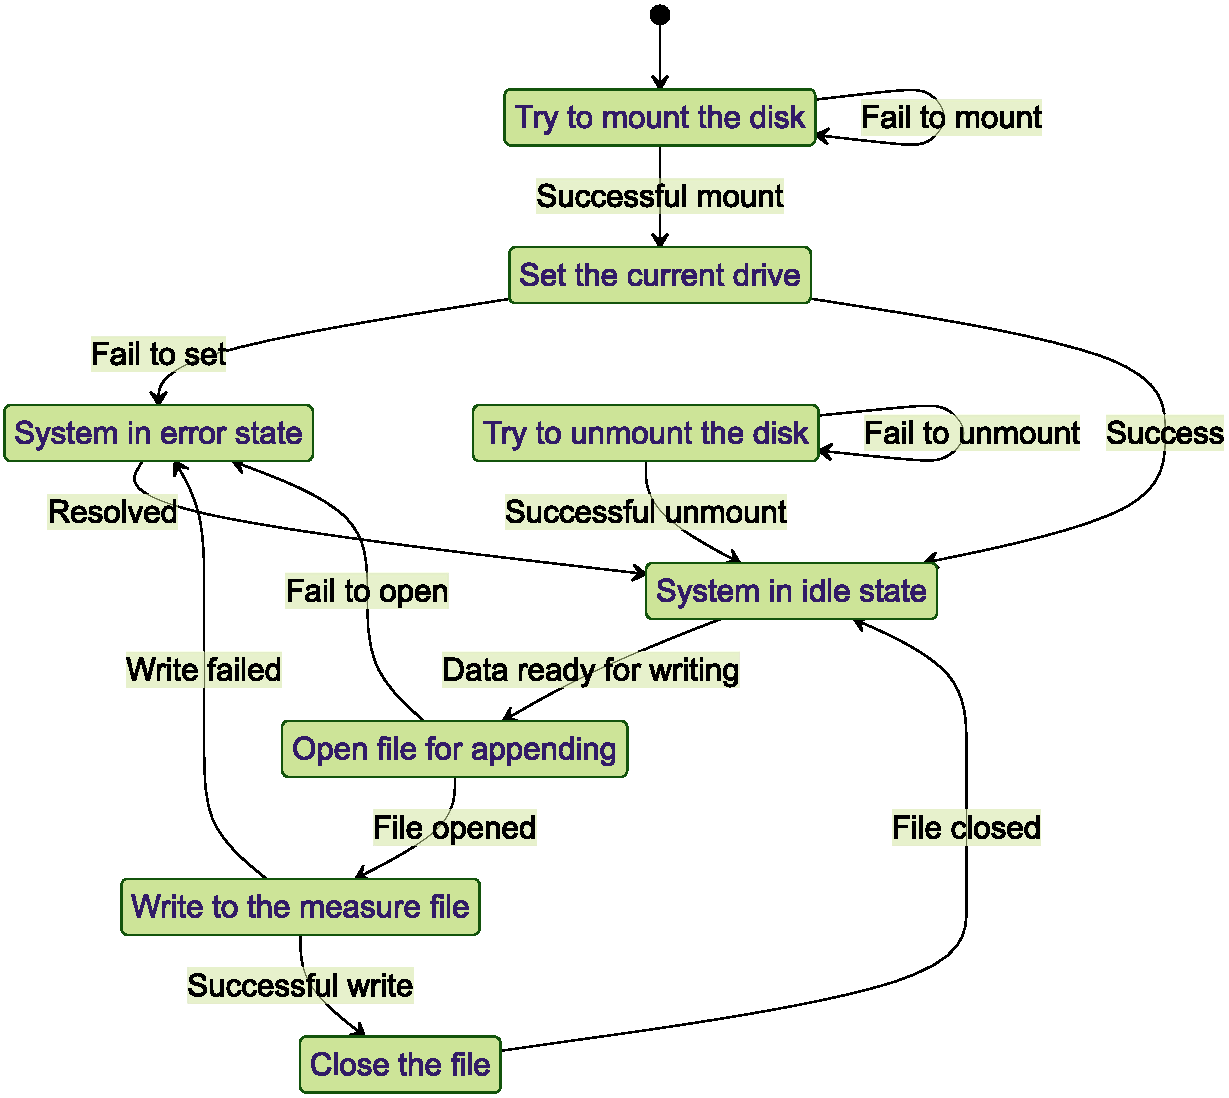
\includegraphics[height=.9\textheight]{../figures/code/diagrammes/sd-card-logging}
	\label{fig:sd-card-logging}
\end{figure}
\end{frame}

\begin{frame}{Enregistrement des données}
\begin{figure}[h]
	\centering
	
\includegraphics[width=0.3\linewidth]{../figures/presentation/micro-sd-card-illustration-material-3-svgrepo-com}
\end{figure}
\begin{figure}[h]
	\centering
	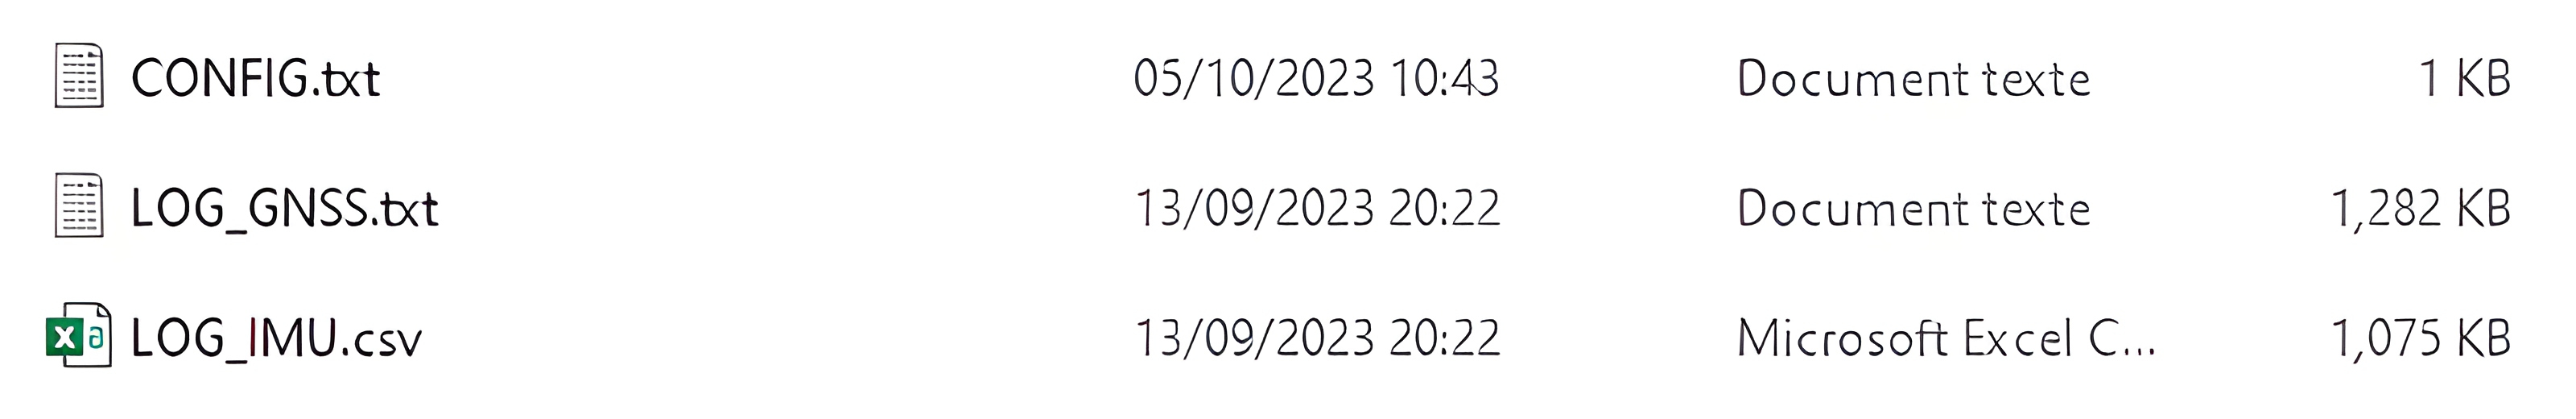
\includegraphics[width=0.9\linewidth]{../figures/presentation/Fichiers-mesures}
\end{figure}
\end{frame}

\begin{frame}{Données CSV - Centrale inertielle}
	\begin{figure}[h]
		\centering
		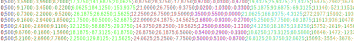
\includegraphics[width=1\linewidth]{../figures/code/donbnees-csv}
	\end{figure}
	\begin{figure}[h]
		\centering
		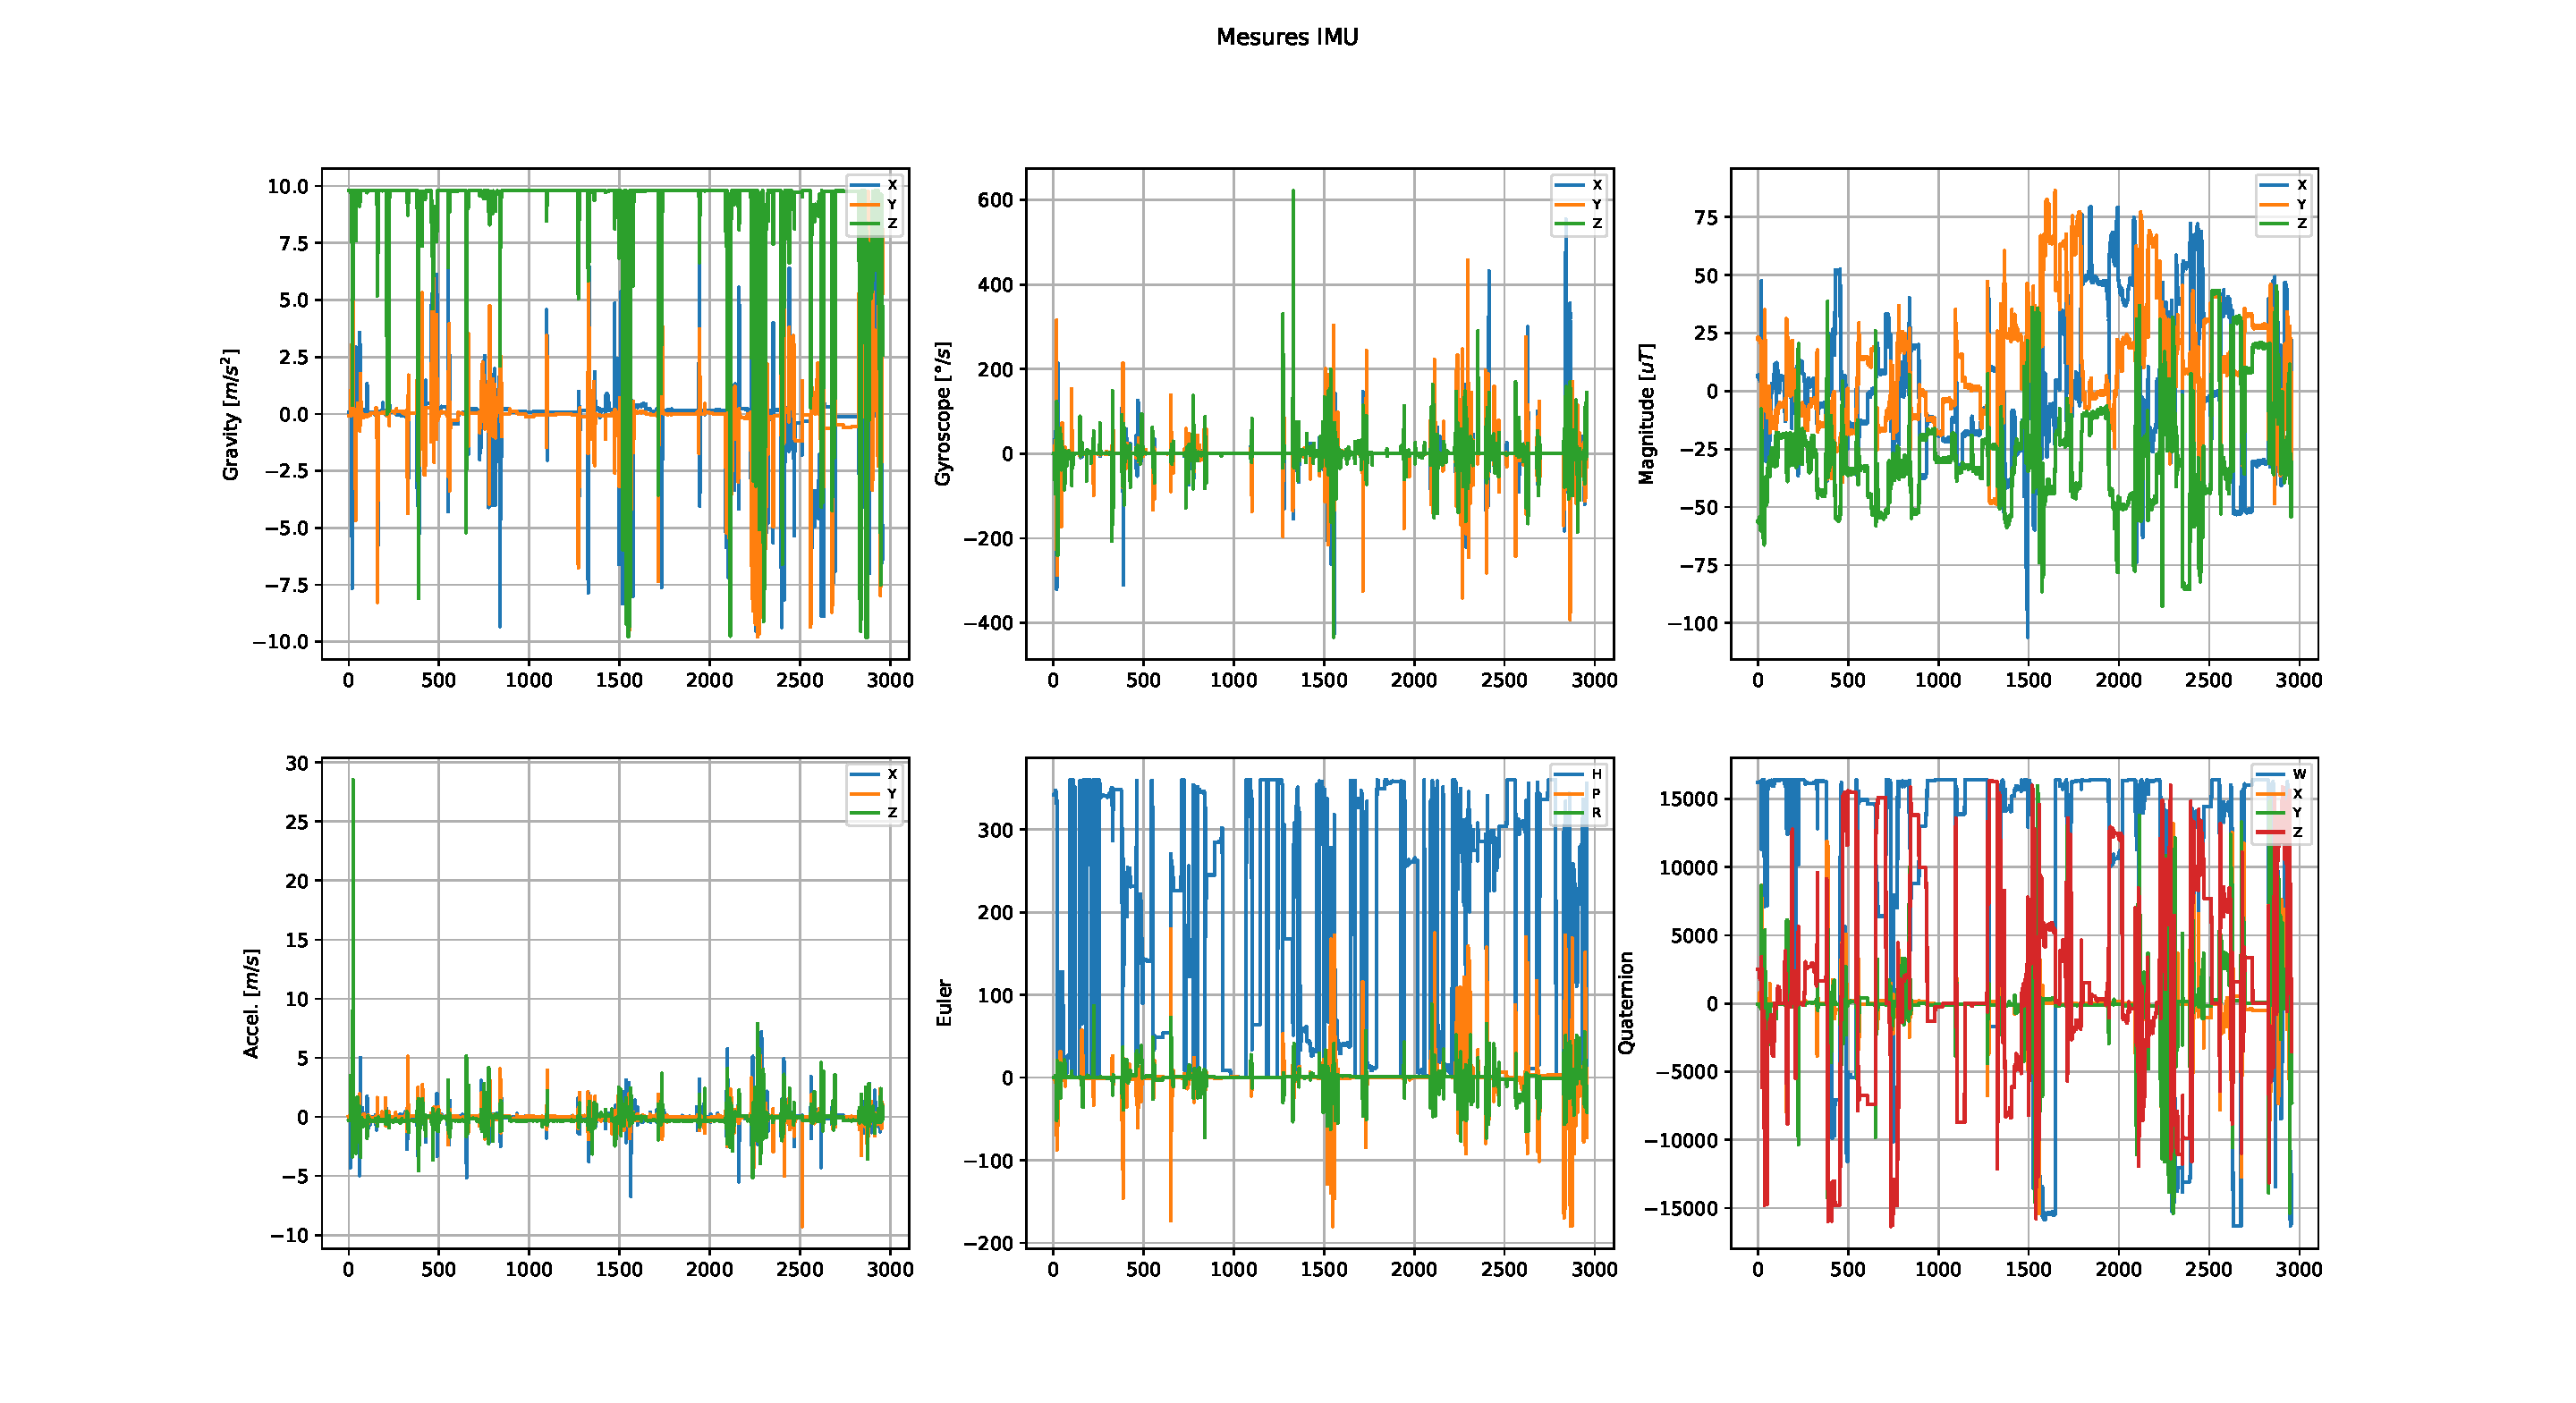
\includegraphics[width=1\linewidth]{../figures/application/mesures}
	\end{figure}
\end{frame}

\begin{frame}{Données NMEA - GNSS}	
	\begin{figure}[h]
		\centering
		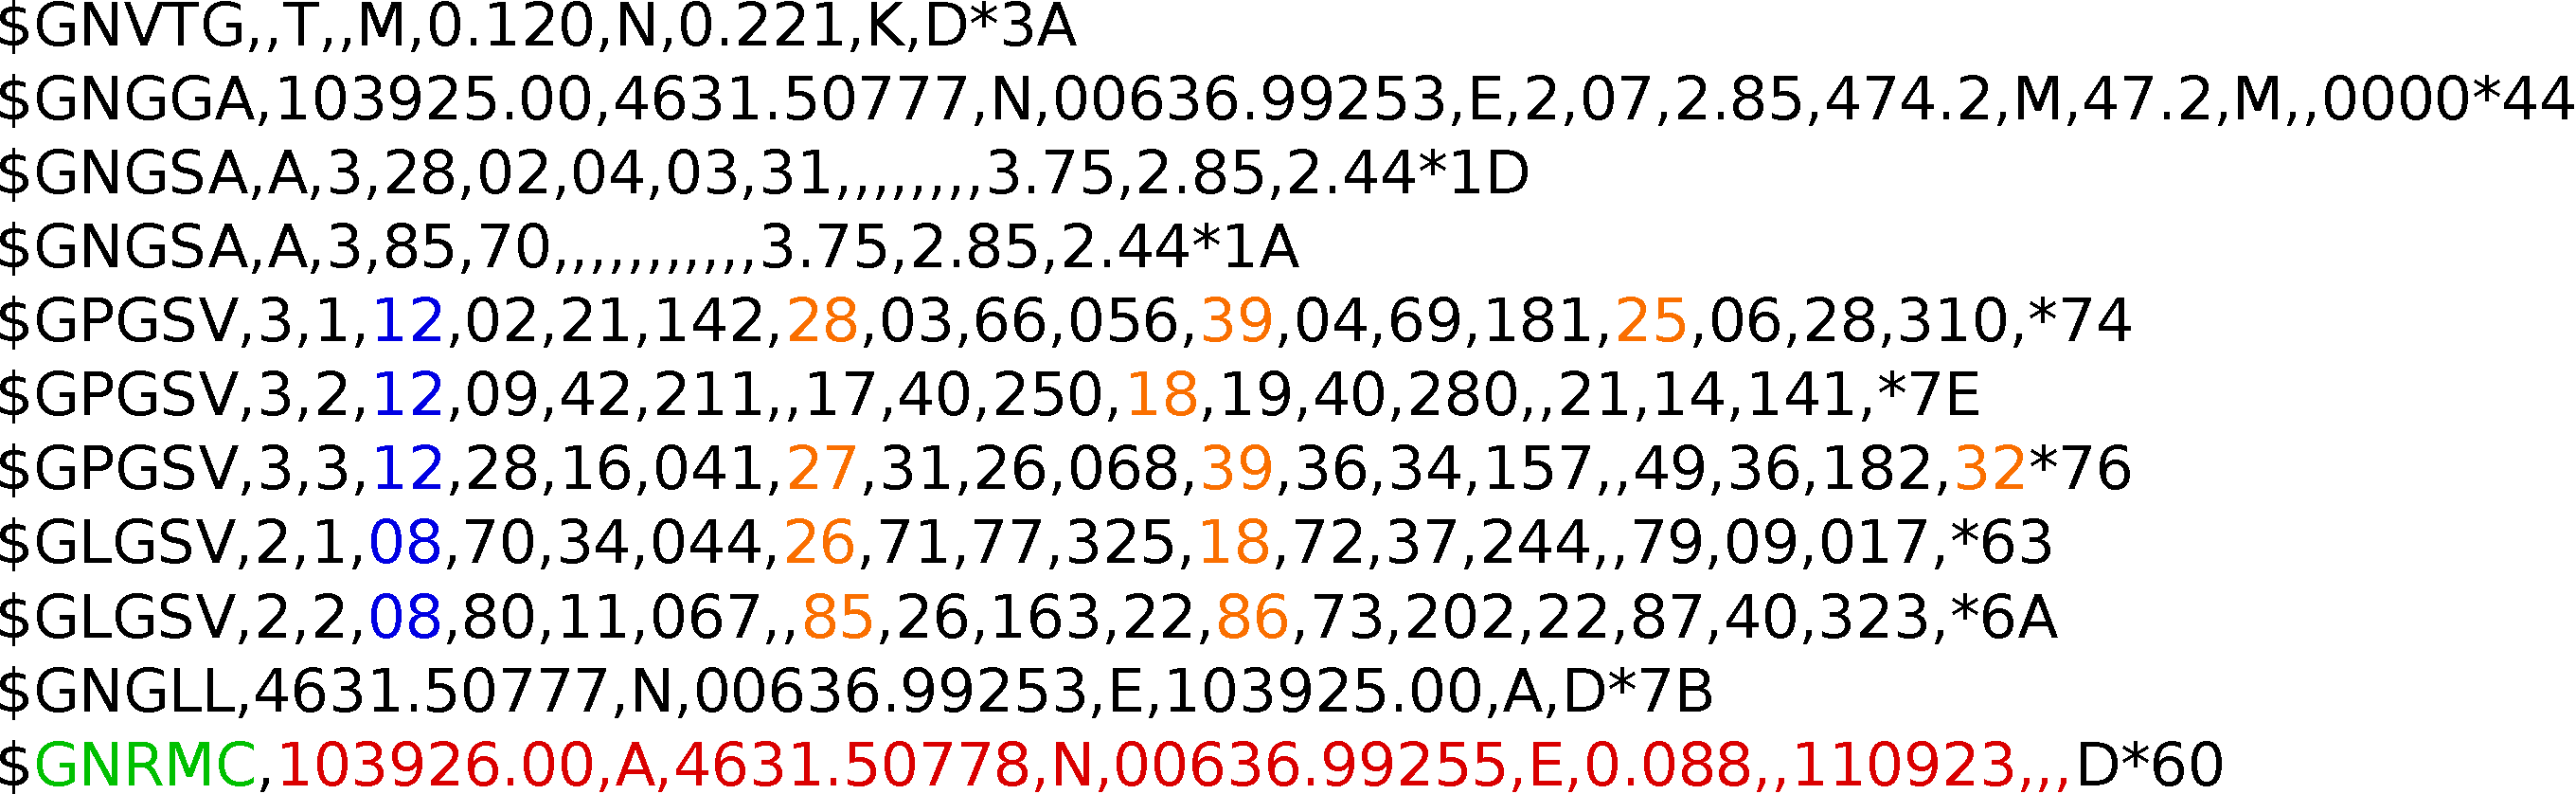
\includegraphics[width=0.9\linewidth]{../figures/presentation/donnees-NMEA}
	\end{figure}
	\begin{figure}[h]
		\centering
		\fbox{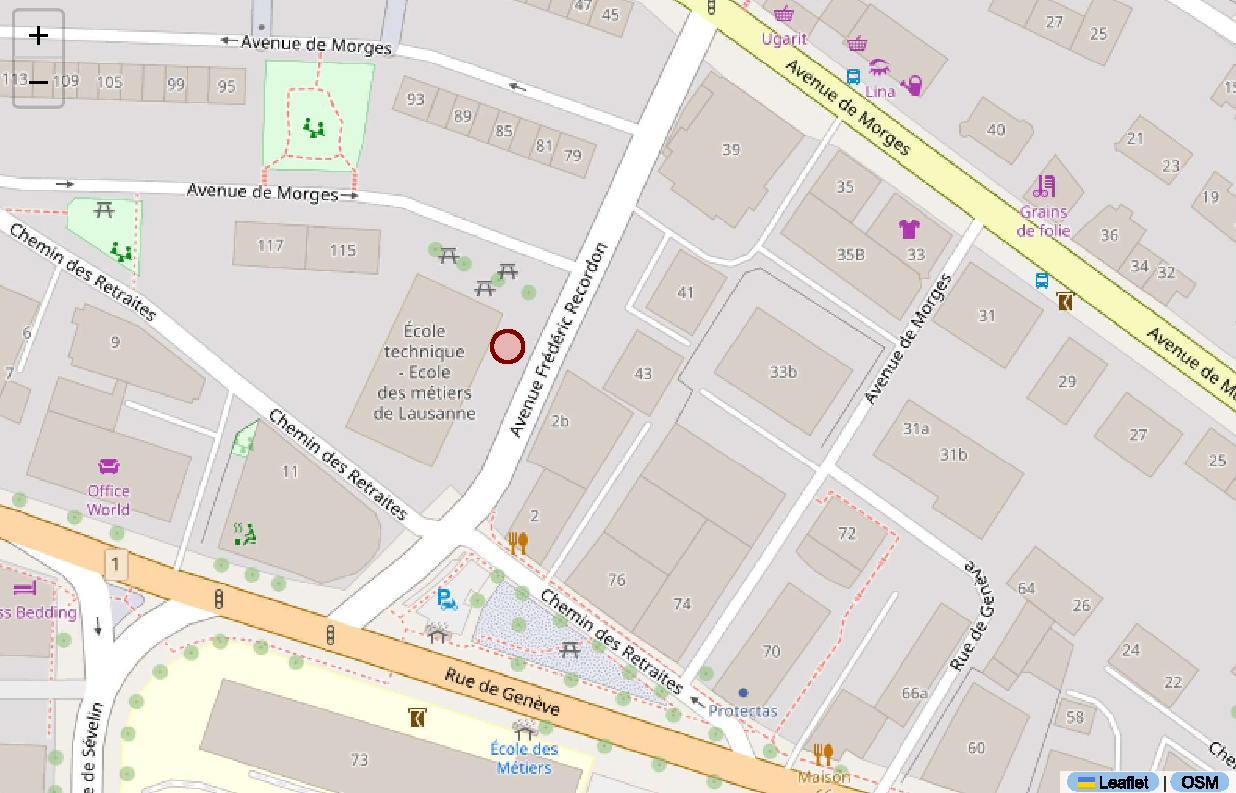
\includegraphics[width=0.5\linewidth]{../figures/presentation/Map}}
	\end{figure}
\end{frame}

\begin{frame}{Fichier de configuration}
	\begin{figure}[h]
		\centering
		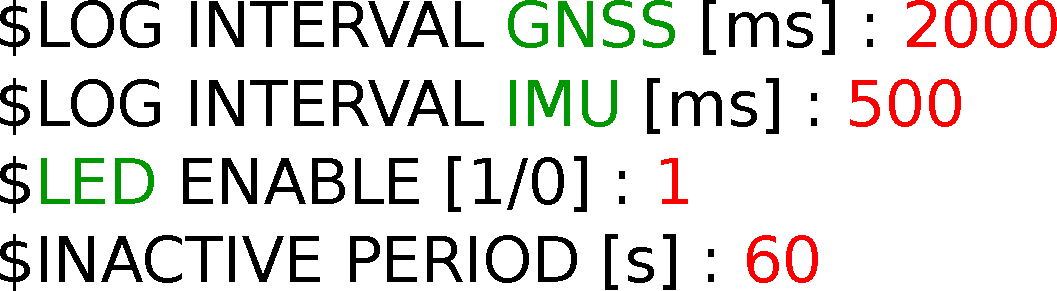
\includegraphics[width=0.7\linewidth]{../figures/presentation/config}
	\end{figure}
\end{frame}

\begin{frame}{Application}
	\begin{figure}[H]
		\centering
		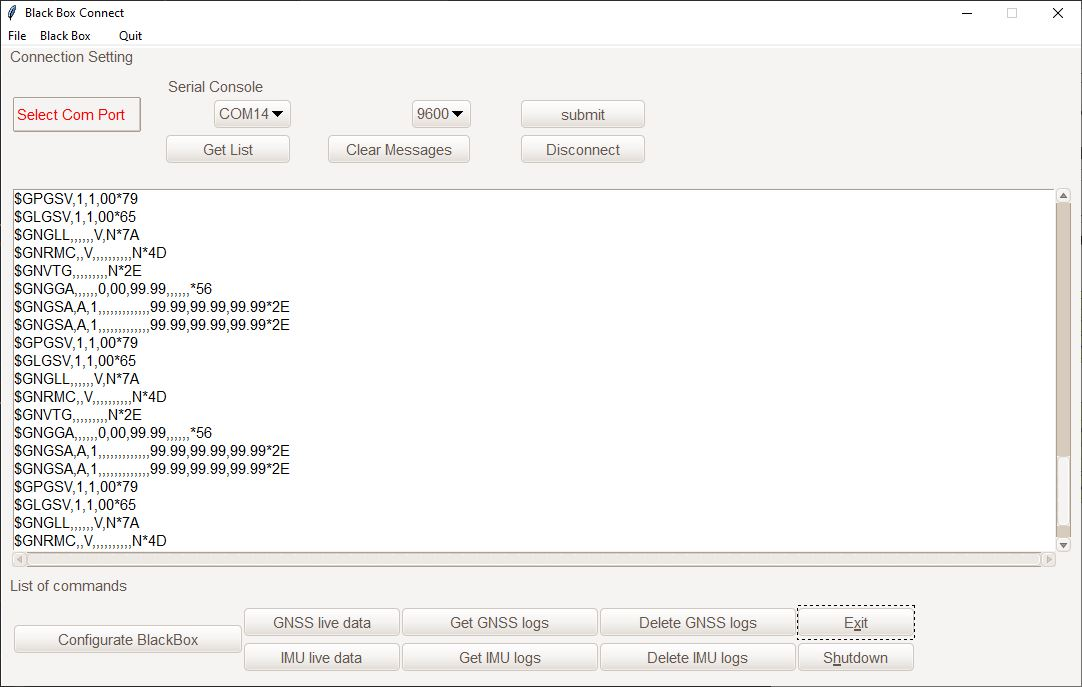
\includegraphics[width=.9\linewidth]{../figures/application/screen_logGnss}
	\end{figure}
\end{frame}


\section{Validation du design}

\begin{frame}{Modifications effectuées}
	Ajout d'un connecteur MHF1 et antenne externe flexible "strip" indépendante du plan de masse.
	
	\begin{figure}
		\centering
		\begin{subfigure}[b]{0.3\textwidth}
			\centering
			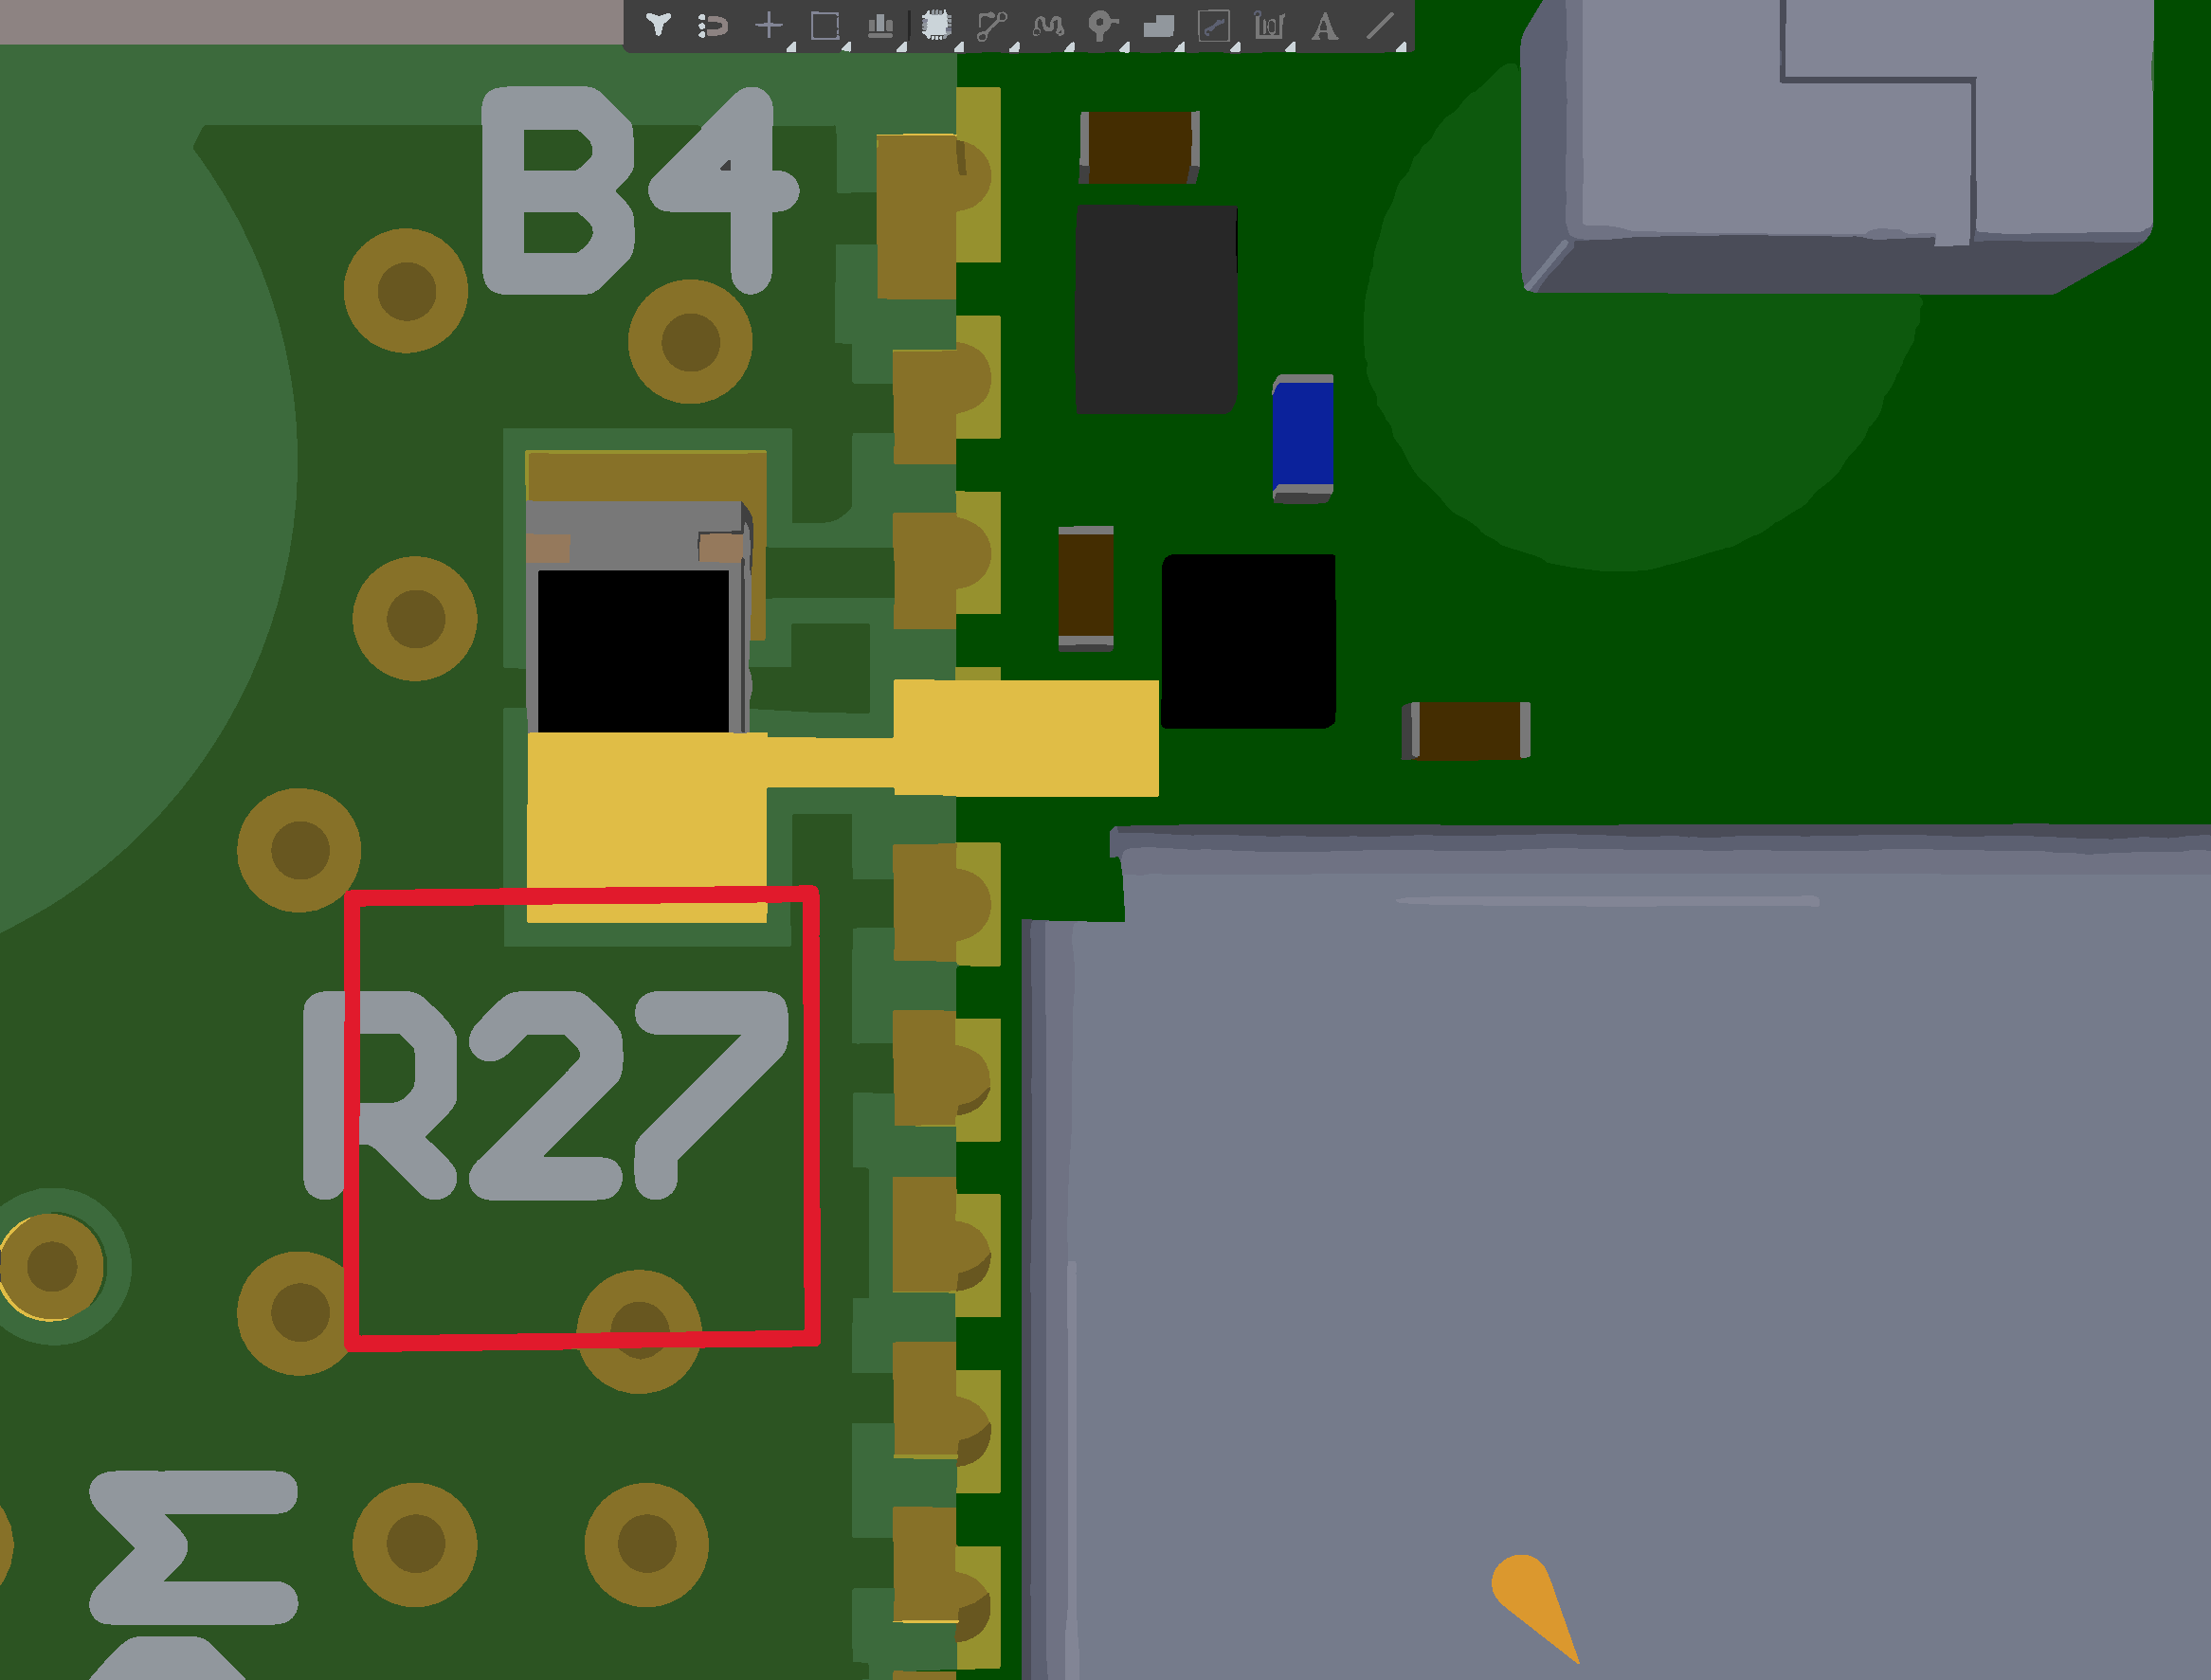
\includegraphics[width=1\linewidth, center]{../figures/presentation/modif}
		\end{subfigure}
		\hfill
		\begin{subfigure}[b]{0.3\textwidth}
			\centering
			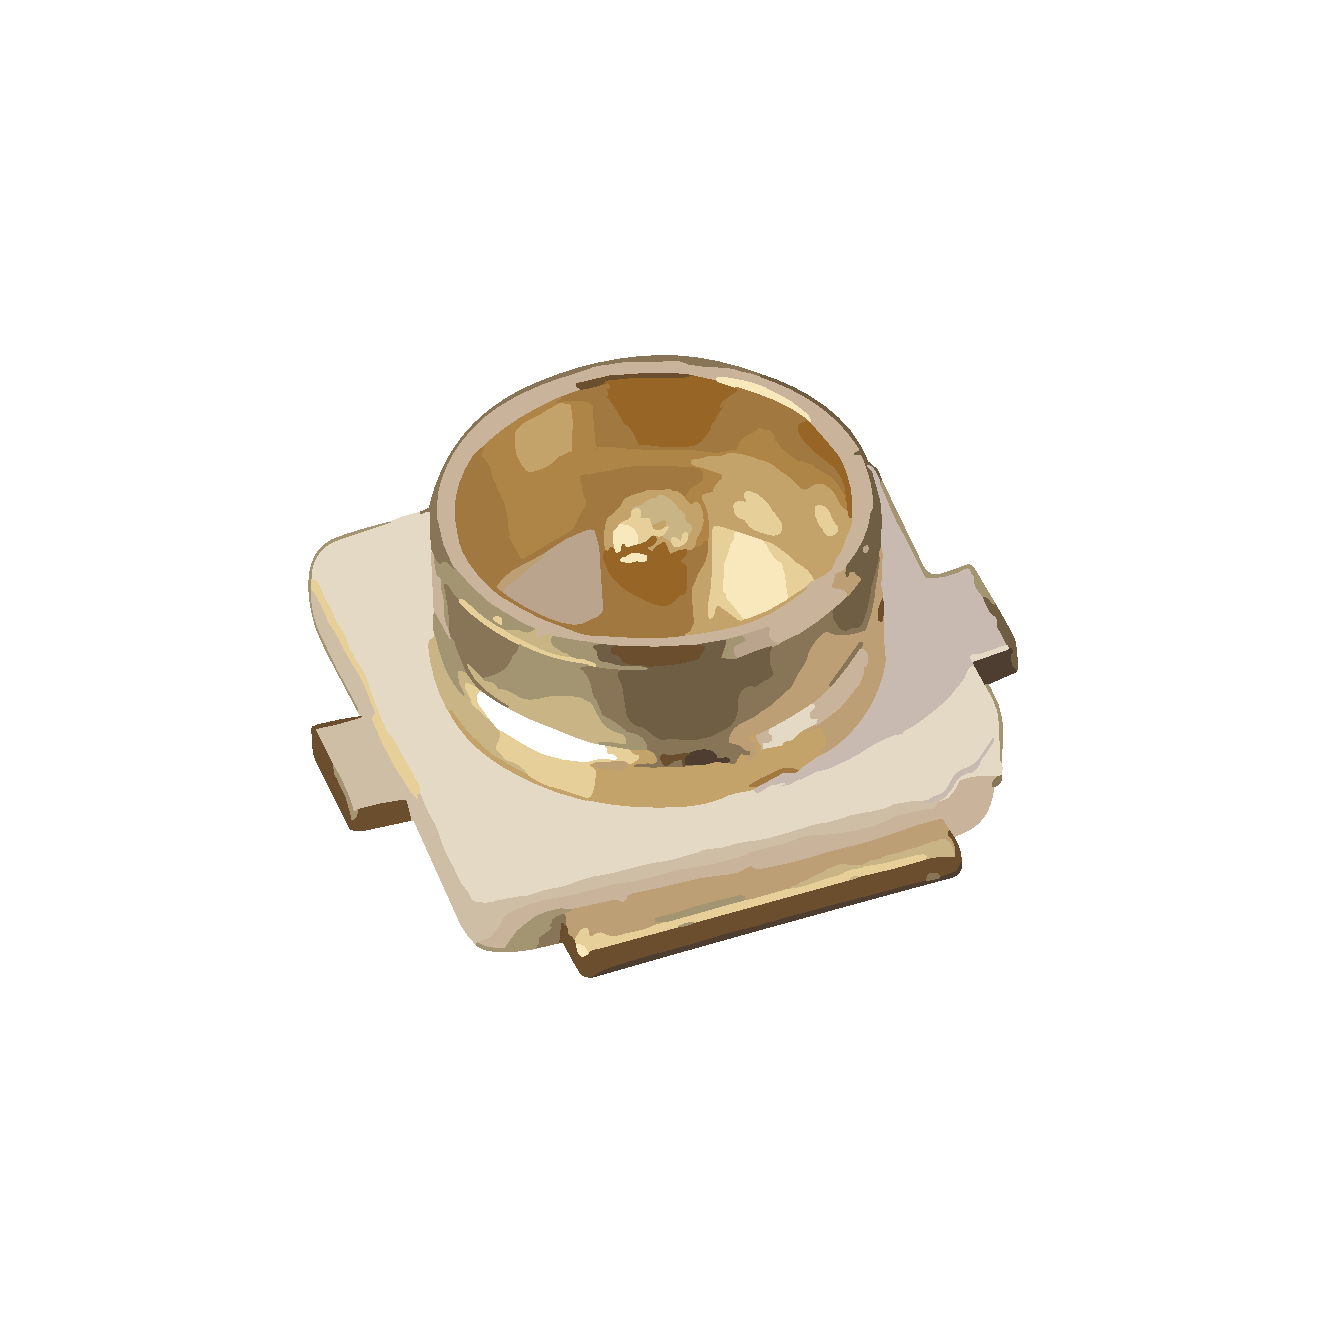
\includegraphics[width=1\linewidth, center]{../figures/presentation/MFG_CONMHF1-SMD-G-T}
		\end{subfigure}
		\hfill
		\begin{subfigure}[b]{0.3\textwidth}
			\centering
			\includegraphics[width=1\linewidth, center]{../figures/presentation/antenne-flex}
		\end{subfigure}
		\hfill
	\end{figure}	
\end{frame}

\begin{frame}{Consommations}
	\begin{table}[!h]
		\centering
		\resizebox{1\textwidth}{!}{%
			\begin{tabular}{|c|l|l|c|c|}
				\hline
				\multicolumn{1}{|l|}{Index} & Etat du système & Condition                      & Courant [mA] & Symbol      \\ \hline
				[1]                         & Eteint.         & Mode auto-enclenchement OFF.   & 0.02         & $I_{off}$   \\ \hline
				[2]                         & Veille.         & Est passé par l'état SHUTDOWN. & 4.4          & $I_{sleep}$ \\ \hline
				[3]                         & Veille brutale.\footnotemark & Pas passé par l'état SHUTDOWN. & 9.56         & $I_{ws}$    \\ \hline
				[4]                         & Initialisation. & -                              & 90           & $I_{init}$  \\ \hline
				[5]                         & Logging.        & -                              & 100          & $I_{log}$   \\ \hline
				[6]                         & Shutdown.       & -                              & 83           & $I_{sh}$    \\ \hline
				[7]                         & Communication.  & USB branché.                   & 0            & $I_{usb}$   \\ \hline
			\end{tabular}%
		}
	\caption{Mesure des consommations}
	\label{tab:mes-cons}
	\end{table}
	\resizebox{1\textwidth}{!}{\begin{tabular}{llll}
		$\bullet$ & Temps de logging &  (Table \ref{tab:mes-cons}-[5]) : & $T_l = \frac{C}{I_{log}} = 16h$. \\
		$\bullet$ & Temps épuisement batterie en veille & (Table \ref{tab:mes-cons}-[2]) : & $T_l = \frac{C}{I_{sleep}} = 364h = 15J$. \\
		$\bullet$ & Temps épuisement en veille brutale & (Table \ref{tab:mes-cons}-[3]) : & $T_l = \frac{C}{I_{ws}} = 167h = 7J$. \\
	\end{tabular}}
	
\end{frame}

\begin{frame}{Bus de communications}
	\resizebox{1\textwidth}{!}{\begin{tabular}{lllll}
		$\bullet$ & I2C & Temps set de mesure IMU & $2.275$ & $[ms]$ \\
		$\bullet$ & UART1 & Temps set de mesure GNSS & $234.4$ & $[ms]$\\
		$\bullet$ & UART1 & Intervalle entre messages NMEA & $1$ & $[s]$\\
		$\bullet$ & UART2 & Temps réaction cmd en mode CONFIG & $120$ & $[\mu s]$\\
		$\bullet$ & UART2 & Temps réaction cmd en mode LOG. & $2.7$ & $[ms]$\\
		$\bullet$ & SPI & Mesure fréquence carte SD & $12.0192$ & $[MHz]$\\
	\end{tabular}}
\end{frame}

\begin{frame}{Caractéristiques finales}
	\begin{table}[h]
		\centering
		\resizebox{.65\textwidth}{!}{%
			\begin{tabular}{|c|cc|}
				\hline
				Caractéristique                                                                       & \multicolumn{2}{c|}{Attribut}               \\ \hline
				Axes de mesures                                                                       & \multicolumn{1}{c|}{9}       & [axes]       \\ \hline
				Mesures IMU & \multicolumn{2}{c|}{\begin{tabular}[c]{@{}c@{}}Temps, Gravité, Gyro, Magnitude,\\ Accél. linaire, Angle de Euler, Quaternions\end{tabular}} \\ \hline
				\begin{tabular}[c]{@{}c@{}}Intervalles mesure GNSS\\ (par défaut)\end{tabular}  & \multicolumn{1}{c|}{5000}    & [ms]         \\ \hline
				\begin{tabular}[c]{@{}c@{}}Intervalles mesure IMU\\ (par défaut)\end{tabular}   & \multicolumn{1}{c|}{500}     & [ms]         \\ \hline
				Capacité carte SD                                                                     & \multicolumn{1}{c|}{256}     & [MB]         \\ \hline
				Nombre de mesures possibles                                                           & \multicolumn{2}{c|}{$1.11*10^6$}            \\ \hline
				Vitesse MCU                                                                     & \multicolumn{1}{c|}{72}      & [MHz]        \\ \hline
				Capacité batterie                                                                     & \multicolumn{1}{c|}{1600}    & [mAh]        \\ \hline
				Autonomie logging                                                                     & \multicolumn{1}{c|}{16}      & [h]          \\ \hline
				Autonomie veille                                                                      & \multicolumn{1}{c|}{2}       & [semaines]   \\ \hline
				Interface                                                                             & \multicolumn{2}{c|}{USB et LED RGB}         \\ \hline
				Communications                                                                        & \multicolumn{2}{c|}{I2C, SPI, UART(2), USB} \\ \hline
				Vitesse SPI                                                                           & \multicolumn{1}{c|}{12}      & [MHz]        \\ \hline
				Vitesse UART 1 et 2                                                                   & \multicolumn{1}{c|}{9600}    & [Bd]         \\ \hline
				Détection accélération > 2G                                                           & \multicolumn{2}{c|}{Oui}                    \\ \hline
				Données satellites                                                                    & \multicolumn{2}{c|}{Date et heure}          \\ \hline
				\begin{tabular}[c]{@{}c@{}}Compensation température\\ (Mesures IMU)\end{tabular} & \multicolumn{2}{c|}{Oui}                    \\ \hline
				Enclenchement automatique                                                             & \multicolumn{2}{c|}{Oui}                    \\ \hline
				Système d'économie d'énergie                                                          & \multicolumn{2}{c|}{Oui}                    \\ \hline
				Application software développée                                                       & \multicolumn{2}{c|}{Oui, "BBX-Connect"}     \\ \hline
			\end{tabular}%
		}
	\end{table}
\end{frame}

\section{Conclusion}
\begin{frame}{Conclusion}
\begin{figure}[h]
	\centering
	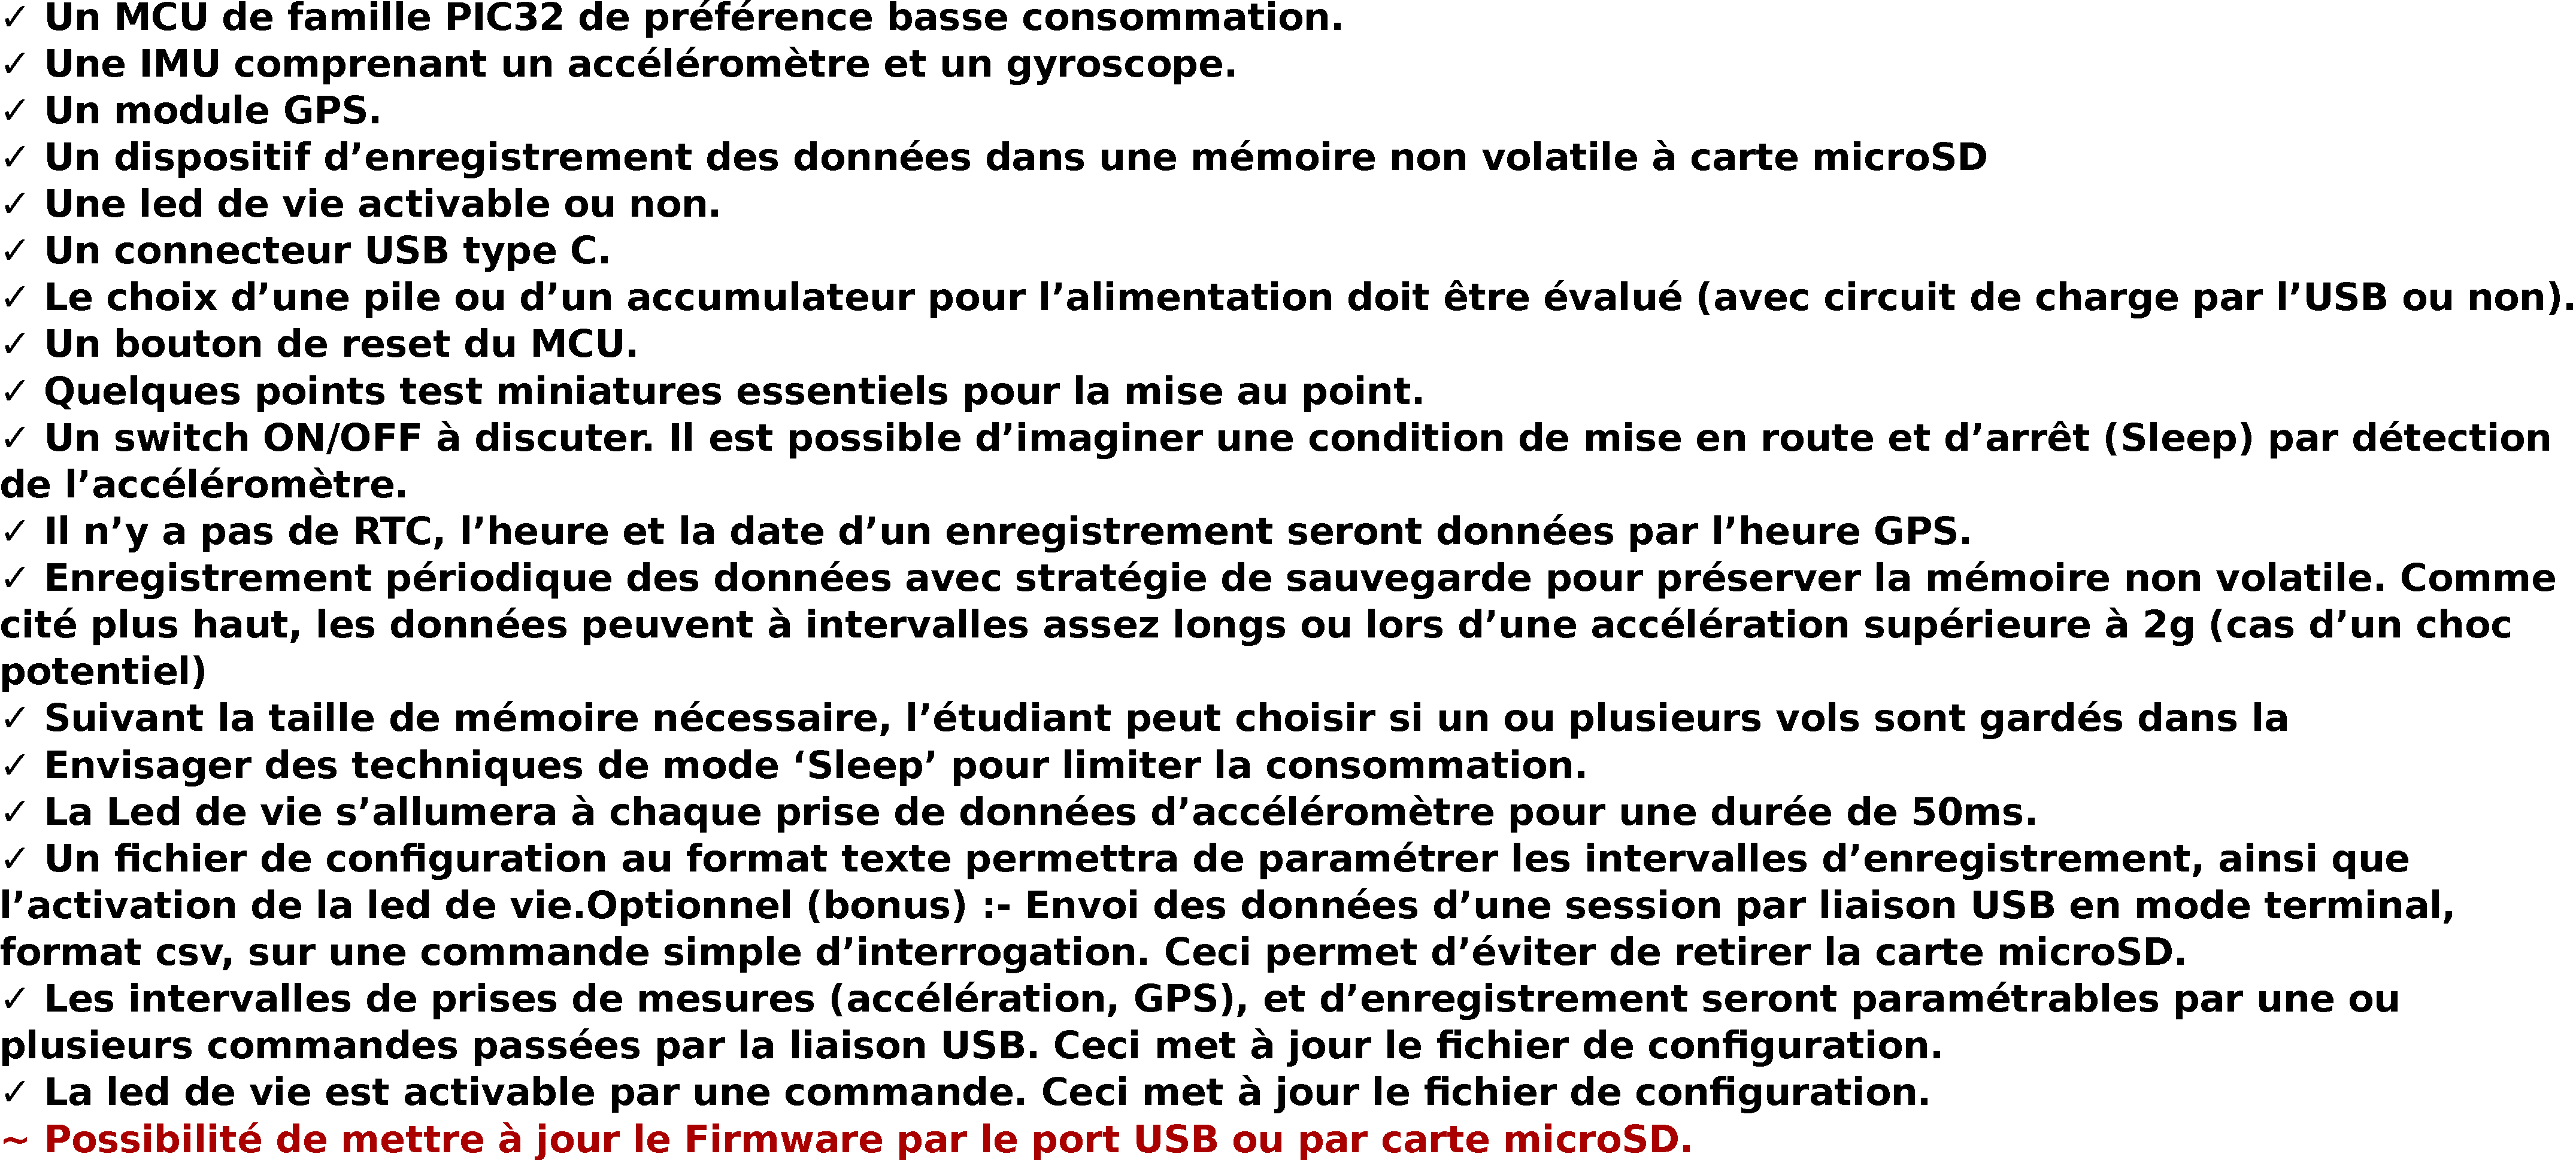
\includegraphics[width=1.08\textwidth]{../figures/presentation/CDC.pdf}
\end{figure}		
\end{frame}

\begin{frame}[standout]
	Questions?
\end{frame}
	
\end{document}
